\chapter{State of the art of QEC codes: Surface codes, color codes and QLDPC codes}
\label{chap:state_of_the_art}

\section{Introduction}
In Chapter 1, we established the fundamental principles of quantum error correction (QEC), learning how we can encode logical information into multiple physical qubits to protect it from noise. However, finding the right code for a real-world quantum computer is a delicate balancing act. A good QEC code must offer high fault-tolerance thresholds and error supression capabilities, require hardware connectivity that is actually physically possible to build, and maintain a reasonable encoding rate so that we do not need a very large number of physical qubits for each logical one we encode. Additionally, the decoding process must run within the bounds imposed by the quantum gate execution times in the actual quantum computer to allow a real-time decoding and correction of errors.

This chapter explores the evolution of these codes, focusing on three major families: Surface codes, Color codes, and Quantum Low-Density Parity-Check (QLDPC) codes.

\subsection{About terminology: Topological vs. LDPC Codes}
\notatfm{In modern literature, when researchers say "QLDPC codes", they are often referring colloquially to \textit{non-topological} QLDPC codes.} Before analyzing specific codes, we must clarify the terminology we use to classify them:
\begin{itemize}
    \item \textbf{Topological Codes:} In a topological code, qubits are arranged on a physical lattice (usually in 2D or 3D). Crucially, the stabilizer checks only interact with strictly local, geometrically adjacent qubits. Surface codes and 2D color codes are the quintessential examples of topological codes.
    \item \textbf{Quantum Low-Density Parity-Check (QLDPC) Codes:} A code is considered LDPC if the number of qubits involved in any single parity check (its weight), and the number of checks acting on any single physical qubit, are both strictly bounded by a constant, regardless of the size of the code. Mathematically, surface codes and color codes perfectly fit this definition.
    \item \textbf{\textit{Non-topological} QLDPC Codes:} These codes sacrifice the strict 2D geometric locality in favor of long-range connections. Doing so allows them to break theoretical limits and achieve asymptotically "good" encoding rates (where the number of logical qubits scales linearly with the physical ones).
\end{itemize}

\section{Transversality and the Eastin-Knill Theorem}

A central goal in Quantum Error Correction (QEC) is executing logical gates fault-tolerantly. A gate is called \textit{transversal} if applying the physical gate independently to each physical data qubit results in the logical version of that gate being applied to the encoded state. Transversal gates are the holy grail of fault-tolerance because they never propagate errors between qubits within the same code block. Because the operations are performed strictly on isolated pairs of physical qubits (qubit-by-qubit), an error cannot spread to other physical qubits within the same logical block. Thus, a single physical error remains a single physical error, which the error-correcting code can safely detect and fix.

However, the \textbf{Eastin-Knill Theorem} \cite{eastin2009restrictions} states a severe theoretical limitation: \textit{No quantum error-correcting code can have a universal set of transversal logical gates}. This means we cannot build a universal quantum computer relying solely on these simple, inherently safe transversal operations. 

When a required logical gate is non-transversal, we cannot simply interact the physical qubits of one logical block with another pairwise. Instead, we must rely on complex fault-tolerant protocols that interact deeply with the internal structure and boundaries of the logical qubits. These protocols are challenging to implement and are prone to causing error propagation. Depending on the nature of the target operation, two main techniques are employed:

\subsection*{Multi-Qubit Gates: Lattice Surgery}
\notatfm{In Lattice Surgery, merging two logical qubits means activating ancillas between the borders of the two logical qubits and creating two qubit gates between these ancillas and data qubits of the two adjacent logical qubits, effectively creating a chain of stabilizers through the boundary of both qubits. The subsequent measurement of these stabilizer chain is equivalent to measuriring the joint logical operator for both qubits. The act of measuring it is what causes the projection that leaves both logical qubits in an entangled state.} To perform non-transversal operations between two distinct logical qubits (for example, a logical CNOT in codes that do not support it transversally), the standard approach is \textbf{Lattice Surgery}. Rather than applying physical gates between individual pairs of qubits across the blocks, lattice surgery temporarily "merges" two distinct logical qubits into one larger logical block by measuring multi-qubit parity checks along the spatial boundary separating them. 

After the logical operation is completed, the blocks are "split" again. While this protocol is fault-tolerant in theory, it is practically demanding. It requires executing delicate measurement cycles along the boundaries of the code patches, demanding extra routing and exposing the logical qubits to complex error propagation dynamics during the merging and splitting phases.

\subsection*{Single-Qubit Gates: Magic State Injection and Distillation}
To implement non-transversal single-qubit gates---most notably the non-Clifford $T$-gate, which is essential for universal quantum computation---we use \textbf{Magic State Injection} \cite{bravyi2005universal}. Instead of applying the gate directly to our data qubit, we prepare an auxiliary logical qubit in a special state called a "magic state". We then entangle our data qubit with this magic state (often using lattice surgery) and measure the auxiliary block, effectively teleporting the non-Clifford operation onto our data.

The critical issue is that preparing a magic state fault-tolerantly directly from physical qubits initially yields a "noisy" state. If we inject a noisy state into our computation, the logical algorithm will fail. Therefore, before injection, these states must be purified using a process called \textbf{Magic State Distillation}. 

Distillation is a highly iterative and wasteful protocol that consumes several noisy magic states to produce a single, higher-fidelity state. For instance, a standard distillation protocol might consume 15 noisy states to yield just 1 usable state. Because useful quantum algorithms require large numbers of $T$-gates, a fault-tolerant quantum computer must continuously manufacture these states in real-time. 

\notatfm{An example of the distillation overhead is visible in the 2021 article by Gidney \& Ekera\cite{Gidney_2021}. In this paper, they propose the factorization of a 2048 bit RSA interger using a quantum processor with 20 million qubits. The article estimates that 25\% of these qubtis should be dedicated to Magic State distilation.} To achieve this, quantum processors must dedicate enormous, specialized regions---often referred to as \textit{Magic State Factories}---exclusively to this task. This immense spatial and temporal overhead is precisely what motivates the search for alternative QEC families. For instance, some configurations of color codes \cite{bombin_martindelgado_2006} inherently support a much richer set of transversal gates, significantly reducing or entirely bypassing the need for extensive magic state distillation.









\section{Surface Codes}

\subsection{From 1D Repetition to 2D Topologies}
In Chapter 1, we learned that a 1D linear repetition code can only protect against one specific type of error (either bit-flips or phase-flips). Historically, protecting against both required complex concatenation schemes, like Shor's 9-qubit code. The surface code solves this elegantly by expanding into a second spatial dimension. By distributing qubits across a 2D grid, the code can interleave two different types of parity checks simultaneously, monitoring both $X$ and $Z$ errors without the recursive and inefficient overhead of concatenation.

\subsection{Origins: The Toric Code}
\notatfm{As formulated by Bombín \& Martín-Delgado \cite{bombin_martindelgado_2007}, surface codes can also be represented as a lattice with colored faces. In this configuration, data qubits reside on the vertices and stabilizers are defined on the faces, with the color of each face indicating the type of stabilizer. This is known as the rotated surface code representation and is now widely adopted in the literature.}
This 2D topological approach was famously introduced by Alexei Kitaev in 1997 via the \textbf{Toric Code} \cite{kitaev2003fault}. It is typically defined on a 2D square lattice where the data qubits reside on the edges. The parity checks (stabilizers) are defined on the vertices ($X$-checks) and the faces or plaquettes ($Z$-checks). In this geometric arrangement, every data qubit is continuously monitored by four ancilla qubits: two responsible for $X$-checks and two for $Z$-checks. Conversely, every ancilla qubit monitors exactly four adjacent data qubits.

This specific topology is not arbitrary; it is meticulously designed to satisfy the fundamental requirement of stabilizer quantum codes: all parity checks must commute. Because $X$ and $Z$ Pauli operators anticommute on a single qubit, an $X$-check and a $Z$-check will only commute if they overlap on an \textit{even} number of shared data qubits. In this lattice geometry, any vertex ($X$-check) and any adjacent face ($Z$-check) will always share exactly two data qubits, ensuring that all operators commute globally and the checks can be measured simultaneously without collapsing the logical state.

To avoid the mathematical complexity of handling open boundaries at the edges of the grid, Kitaev imagined a lattice with periodic boundary conditions. In this model, the top edge of the lattice connects to the bottom edge, and the left edge connects to the right edge. Topologically, joining these opposing edges forms a continuous closed surface in the shape of a torus. 

\subsection{Observables, Capacity, and Code Distance}
In topological codes, logical operations (logical gates and measurements of the qubit) are not applied to single physical qubits. Instead, logical observables are defined as continuous chains or \textit{strings} of Pauli operators applied sequentially along a path of adjacent data qubits. 

A closed string of operations that forms a small, trivial loop on the surface is simply a combination of stabilizers and has no effect on the encoded logical state. However, a string that wraps entirely around the torus---a \textit{non-contractible loop}---fundamentally changes the logical state. These global, non-contractible strings represent our logical operators ($X_L$ and $Z_L$). Figure \ref{fig:2:surface_code_evolution} shows this.

When visualizing this topology on a 2D grid, these two distinct non-contractible loops correspond to the orthogonal directions of the lattice (East-West and North-South). On a torus, for each of these two directions, two operators, $X_L$ and $Z_L$, can be applied, effectively codifying 2 qubits (each with 2 operators).

The number of logical qubits $k$ a code can store depends strictly on the topology (the genus) of the surface. A torus has exactly two independent paths to wrap a string (one around the central hole, and one through the tube), meaning the toric code natively encodes exactly $k=2$ logical qubits, regardless of its physical size. We can therefore characterize this toric code as a $[[2d^2, 2, d]]$ code.

To increase the protection of the code, we simply increase the density of the grid. By adding more physical qubits, the topological shape (the torus) remains identical, but the length of the shortest non-contractible string grows. This minimum string length is exactly the \textbf{code distance} ($d$). As the grid grows, it takes a longer chain of consecutive physical errors to accidentally form a logical operator, thereby increasing the fault-tolerance while preserving the underlying topological properties.

\subsection{Planar Implementation and Rotated Surface Codes}
While the toric code is mathematically beautiful, manufacturing a quantum processor shaped like a 3D torus is physically impractical, particularly for 2D planar architectures like superconducting circuits. 

To implement this on a real chip, we must "cut" the torus and lay it flat. This physical cut transforms the Toric Code into the planar \textbf{Surface Code}. However, cutting the torus exposes physical borders. To preserve the ability to correct both $X$ and $Z$ errors, the planar patch must have two types of alternating boundaries: "rough" boundaries (where $Z$-strings terminate) and "smooth" boundaries (where $X$-strings terminate). Because the closed loops of the torus are now severed into linear strings that span from one boundary to the opposite, the storage capacity drops: a standard planar patch encodes only $k=1$ logical qubit.

To further optimize the mapping onto real hardware, the planar surface code is almost universally implemented in its \textbf{rotated} version. While this rotated representation perfectly preserves the underlying topological properties, it drastically improves spatial efficiency. Because the code distance $d$ is defined purely by the minimum length of the string connecting opposite boundaries, rotating the orientation of these boundaries by 45 degrees eliminates the wasted corner qubits present in the standard planar cut. Consequently, the rotated surface code requires significantly less physical qubits to achieve the exact same distance $d$ (see Figure \ref{fig:2:surface_code_evolution}).

\begin{figure}[hbt!]
    \centering
    % Subfigure A: Torus with observables
    \begin{subfigure}[b]{0.32\textwidth}
        \centering
        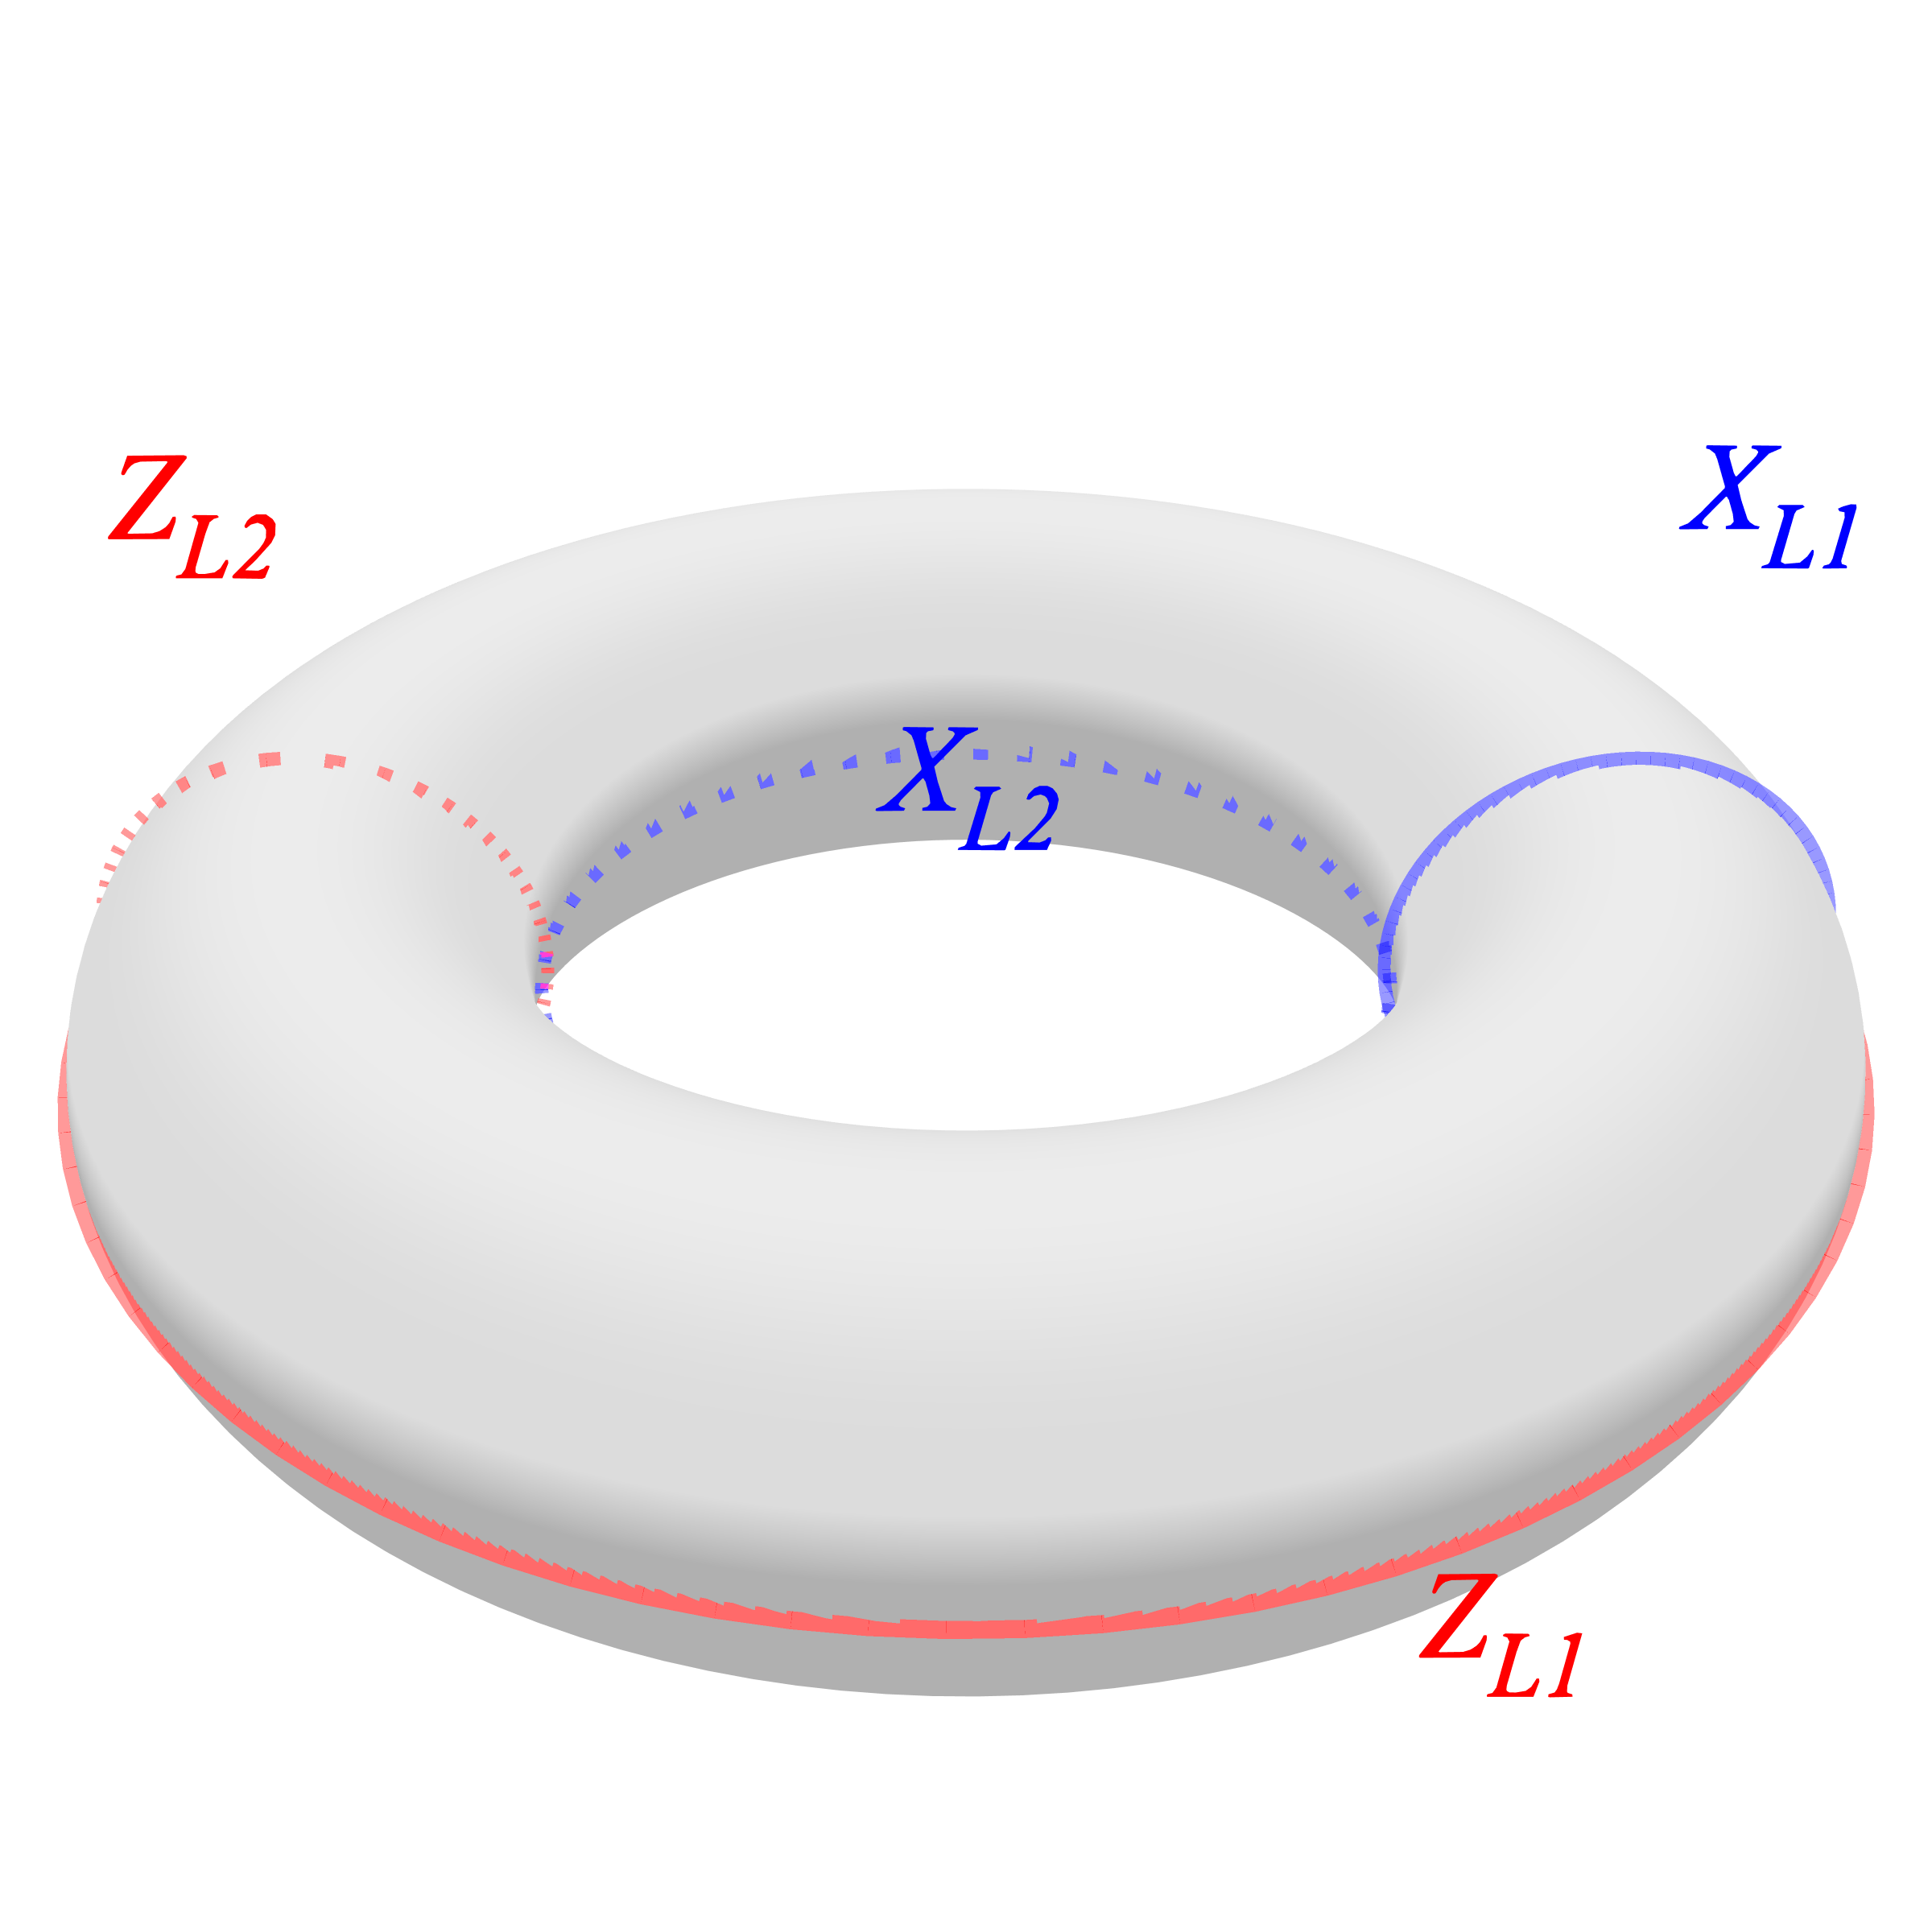
\includegraphics[width=1\linewidth]{figures/chapter_2/c2_torus_kitaev.png}
        \caption{}
    \end{subfigure}
    \hfill
    % Subfigure B: Kitaev's original formulation
    \begin{subfigure}[b]{0.3\textwidth}
        \centering
        
                \begin{tikzpicture}[scale=0.9]
            % Draw the main grid lines (the lattice)
            \draw[gray!60, thick] (0,0) grid (3,3);
        
            % Highlight Z-stabilizer (Plaquette)
            % Picked the bottom-left plaquette 
            \filldraw[red!20, draw=red, ultra thick] (0,0) rectangle (1,1);
            
            % Highlight X-stabilizer (Vertex)
            % Picked an internal vertex at (1,2)
            \draw[blue, ultra thick] (0.5,2) -- (1.5,2);
            \draw[blue, ultra thick] (1,1.5) -- (1,2.5);
        
            % Draw ALL Z-ancillas (Faces) as solid black dots
            \foreach \x in {0.5, 1.5, 2.5} {
                \foreach \y in {0.5, 1.5, 2.5} {
                    \filldraw[black] (\x,\y) circle (2pt);
                }
            }
            
            % Draw ALL X-ancillas (Vertices) as solid black dots
            \foreach \x in {0, 1, 2, 3} {
                \foreach \y in {0, 1, 2, 3} {
                    \filldraw[black] (\x,\y) circle (2pt);
                }
            }
        
            % Overwrite the active ancillas with their respective colors (no text)
            \filldraw[blue] (1,2) circle (3pt);
            \filldraw[red] (0.5, 0.5) circle (3pt);
        
            % Draw data qubits on all horizontal edges (white filled circles)
            \foreach \x in {0.5, 1.5, 2.5} {
                \foreach \y in {0, 1, 2, 3} {
                    \filldraw[black, fill=white, thick] (\x,\y) circle (2.5pt);
                }
            }
            % Draw data qubits on all vertical edges (white filled circles)
            \foreach \x in {0, 1, 2, 3} {
                \foreach \y in {0.5, 1.5, 2.5} {
                    \filldraw[black, fill=white, thick] (\x,\y) circle (2.5pt);
                }
            }
        
            % Fill the specific data qubits involved in the highlighted X check to make them pop
            \filldraw[blue] (0.5,2) circle (3pt);
            \filldraw[blue] (1.5,2) circle (3pt);
            \filldraw[blue] (1,1.5) circle (3pt);
            \filldraw[blue] (1,2.5) circle (3pt);
        
            % Fill the specific data qubits involved in the highlighted Z check to make them pop
            \filldraw[red] (0.5,0) circle (3pt);
            \filldraw[red] (0.5,1) circle (3pt);
            \filldraw[red] (0,0.5) circle (3pt);
            \filldraw[red] (1,0.5) circle (3pt);
        
            % Draw Logical Operators (Strings) as OVERLAYS (drawn last)
            % Z_L is a path on the primal lattice (horizontal, lowered to y=2)
            \draw[red, line width=8pt, opacity=0.4] (0, 2) -- (3, 2) node[right, opacity=1, font=\bfseries] {$Z_L$};
            % X_L is a path on the dual lattice (vertical)
            \draw[blue, line width=8pt, opacity=0.4] (2.5, -0.2) -- (2.5, 3.2) node[above, opacity=1, font=\bfseries] {$X_L$};
        \end{tikzpicture}

        \caption{}
    \end{subfigure}
    \hfill
    % Subfigure C: Rotated surface code
    \begin{subfigure}[b]{0.33\textwidth}
        \centering
                \begin{tikzpicture}[scale=0.7]
            % Z-stabilizers (Red full faces)
            \foreach \x/\y in {0/0, 2/0, 1/1, 0/2, 2/2} {
                \filldraw[red!20, draw=red, thick] (\x,\y) rectangle (\x+1, \y+1);
            }
            
            % Z-stabilizers (Red half faces - Rough boundaries left/right)
            \filldraw[red!20, draw=red, thick] (0,1) -- (0,2) -- (-0.5, 1.5) -- cycle; 
            \filldraw[red!20, draw=red, thick] (3,1) -- (3,2) -- (3.5, 1.5) -- cycle; 
        
            % X-stabilizers (Blue full faces)
            \foreach \x/\y in {1/0, 0/1, 2/1, 1/2} {
                \filldraw[blue!20, draw=blue, thick] (\x,\y) rectangle (\x+1, \y+1);
            }
            
            % X-stabilizers (Blue half faces - Smooth boundaries top/bottom)
            \foreach \x in {0, 2} {
                \filldraw[blue!20, draw=blue, thick] (\x,0) -- (\x+1,0) -- (\x+0.5, -0.5) -- cycle;
                \filldraw[blue!20, draw=blue, thick] (\x,3) -- (\x+1,3) -- (\x+0.5, 3.5) -- cycle;
            }
        
            % Ancilla Qubits (Solid black dots)
            % Z full ancillas
            \foreach \x/\y in {0.5/0.5, 2.5/0.5, 1.5/1.5, 0.5/2.5, 2.5/2.5} {
                \filldraw[black] (\x,\y) circle (1.5pt);
            }
            % Z half ancillas
            \filldraw[black] (-0.16, 1.5) circle (1.5pt);
            \filldraw[black] (3.16, 1.5) circle (1.5pt);
        
            % X full ancillas
            \foreach \x/\y in {1.5/0.5, 0.5/1.5, 2.5/1.5, 1.5/2.5} {
                \filldraw[black] (\x,\y) circle (1.5pt);
            }
            % X half ancillas
            \foreach \x in {0.5, 2.5} {
                \filldraw[black] (\x, -0.16) circle (1.5pt);
                \filldraw[black] (\x, 3.16) circle (1.5pt);
            }
        
            % Data Qubits (White filled circles on vertices)
            \foreach \x in {0, 1, 2, 3} {
                \foreach \y in {0, 1, 2, 3} {
                    \filldraw[black, fill=white, thick] (\x,\y) circle (2.5pt);
                }
            }
        
            % Logical Operators (Strings) OVERLAYS
            % Z_L: horizontal red string connecting Left to Right through y=1
            \draw[red, line width=8pt, opacity=0.4] (-0.3, 1) -- (3.3, 1) node[right, opacity=1, font=\bfseries] {$Z_L$};
            
            % X_L: vertical blue string connecting Top to Bottom through x=1
            \draw[blue, line width=8pt, opacity=0.4] (1, -0.3) -- (1, 3.3) node[above, opacity=1, font=\bfseries] {$X_L$};
        
        \end{tikzpicture}

        \caption{}
    \end{subfigure}

    \caption[Evolution and representations of the surface code.]{Evolution and representations of the surface code. \textbf{(a)} The toric code representation, illustrating how logical observables correspond to non-contractible continuous strings wrapping around the two fundamental cycles of the torus. \textbf{(b)} The original planar formulation by Kitaev ($d=4$), with data qubits on the edges and checks on vertices and faces. The red square represents a $Z$-stabilizer and the blue cross represents a $X$-stabilizer. A total of 49 physical qubits are needed. \textbf{(c)} The equivalent rotated surface code, placing data on vertices and alternating checks on colored faces to significantly reduce physical overhead. Red faces represent $Z$-stabilizers and blue faces represent $X$-stabilizers. The blue and red lines represent the minimum string for the respective operators. In this case, only 31 physical qubits are required. In figures \textbf{(b)} and \textbf{(c)} for a $d=4$ code, white circles represent data qubits and black circles represent ancilla qubits.  The blue and red lines represent the minimum strings for the respective logical operators.}
    \label{fig:2:surface_code_evolution}
\end{figure}

\subsection{Advantages and Disadvantages}
The surface code's primary advantage is its high error threshold (around $\sim 1\%$ for circuit-level noise, see \cite{Wang_surface_1percent}) and its locality, relying on strictly nearest-neighbor 2D grid connectivity. This spatial locality is perfectly aligned with the 2D fabrication constraints of modern planar architectures, making it the industry standard baseline.

However, its main disadvantage is its terrible encoding rate. A standard planar surface code patch encodes exactly one logical qubit ($k=1$), regardless of how much we scale its distance $d$. To achieve higher distances and exponentially better protection, the physical footprint grows quadratically ($n \approx d^2$). This massive spatial overhead limits the scalability of surface codes for algorithms requiring thousands of logical qubits when large distances are needed to mitigate physical error.

\section{Color Codes}

\subsection{Origins and Topologies}
\notatfm{A trivalent lattice is a lattice in which each vertex is connected to exactly three edges. A 3-colorable lattice is one where, using only 3 colors, faces can be colored so that two adjacent faces never share the same color.}
Introduced by Bombín and Martin-Delgado \cite{bombin_martindelgado_2006}, topological color codes represent a powerful evolution in the landscape of quantum error correction. They are defined on 2D lattices that strictly satisfy two geometric properties: they must be 3-valent and 3-colorable (typically utilizing red, green, and blue).

Unlike the surface code, which physically separates $X$-checks and $Z$-checks by placing them on vertices and faces respectively, color codes place both $X$ and $Z$ checks on the same faces of the lattice, while data qubits reside exclusively on the vertices. 

This overlapping check structure is mathematically robust due to the inherent geometry of these lattices. In any 3-valent, 3-colorable lattice, every face is guaranteed to have an even number of vertices. Consequently, an $X$-check and a $Z$-check defined on the exact same face will overlap on an even number of data qubits, guaranteeing that they commute. Furthermore, any two adjacent faces will always share exactly one edge (which contains exactly two vertices). Thus, an $X$-check on one face will always share two data qubits with a $Z$-check on an adjacent face, ensuring global commutativity across the entire code block, as required by the Stabilizer Formalism presented in Section \ref{sec:stabilizer_formalism}.

\subsection{2D Color Code Configurations}
\notatfm{While there are only three uniform tilings, an infinite number of 3-valent, 3-coloreable lattices can be defined if uniformity is not required. These are rarely studied in the literature because they are more difficult to scale and fit on a quantum chip with a regular pattern and because their error correction properties are less predictable.} Because of the strict mathematical requirement that the lattice must be 3-valent and 3-colorable, there is only a finite number of uniform tilings (Archimedean tilings) in the 2D plane that can support a color code, see \cite{landahl2011fault}. Specifically, there are exactly three configurations, shown in Figure \ref{fig:2:color_code_lattices}:

\begin{itemize}
    \item \textbf{6.6.6 Lattice:} A regular lattice composed entirely of hexagons. This lattice can be characterized as $\left[\left[ \frac{3d^2 + 1}{4}, 1, d \right]\right]$.
    \item \textbf{4.8.8 Lattice:} A semi-regular lattice where each vertex connects a square and two octagons. It can be characterized as $\left[\left[ \frac{d^2 + 2d - 1}{2}, 1, d \right]\right]$.
    \item \textbf{4.6.12 Lattice:} A more complex semi-regular lattice composed of squares, hexagons, and dodecagons, characterized as $\left[\left[ \frac{3d^2 - 6d + 5}{2}, 1, d \right]\right]$. While theoretically interesting, its extremely high-weight stabilizers (weight-12) make it practically nonviable for current hardware.
\end{itemize}

\begin{figure}[htbp]
    \centering

    \begin{subfigure}[b]{0.3\textwidth}
        \centering
                \begin{tikzpicture}[scale=0.55]
            \def\R{1.2}
            \def\dX{2.07846} 
            
            \colorlet{colR}{red!20}
            \colorlet{colG}{green!20}
            \colorlet{colB}{blue!20}
        
            \newcommand{\hex}[1]{
                \filldraw[fill=#1, draw=black, thick] 
                    (30:\R) -- (90:\R) -- (150:\R) -- 
                    (210:\R) -- (270:\R) -- (330:\R) -- cycle;
            }
        
            % Central hexagon
            \begin{scope}
                \hex{colR}
                \foreach \a in {30, 90, 150, 210, 270, 330} {
                    \filldraw[black, fill=white, thick] (\a:\R) circle (2.5pt);
                }
            \end{scope}
        
            % Surrounding hexagons
            \foreach \cAngle/\col in {0/colG, 60/colB, 120/colG, 180/colB, 240/colG, 300/colB} {
                \begin{scope}[shift={(\cAngle:\dX)}]
                    \hex{\col}
                    \foreach \a in {30, 90, 150, 210, 270, 330} {
                        \filldraw[black, fill=white, thick] (\a:\R) circle (2.5pt);
                    }
                \end{scope}
            }
        \end{tikzpicture}

        \caption{}
        \label{fig:2:lattice_666}
    \end{subfigure}
    \hfill
    \begin{subfigure}[b]{0.3\textwidth}
        \centering
                \begin{tikzpicture}[scale=0.7]
            % L = distance between centers of adjacent squares/octagons
            \def\L{1.3657} 
            
            \colorlet{colR}{red!20}
            \colorlet{colG}{green!20}
            \colorlet{colB}{blue!20}
        
            % Macro for drawing a Square and its 4 data qubits
            \newcommand{\sq}[3]{
                \filldraw[fill=#3, draw=black, thick]
                    ({#1 - 0.4}, {#2 - 0.4}) --
                    ({#1 + 0.4}, {#2 - 0.4}) --
                    ({#1 + 0.4}, {#2 + 0.4}) --
                    ({#1 - 0.4}, {#2 + 0.4}) -- cycle;
                
                \foreach \vx/\vy in {-0.4/-0.4, 0.4/-0.4, 0.4/0.4, -0.4/0.4} {
                    \filldraw[black, fill=white, thick] ({#1 + \vx}, {#2 + \vy}) circle (2.5pt);
                }
            }
        
            % Macro for drawing an Octagon and its 8 data qubits
            \newcommand{\oct}[3]{
                \filldraw[fill=#3, draw=black, thick]
                    ({#1 - 0.4}, {#2 - 0.9657}) --
                    ({#1 + 0.4}, {#2 - 0.9657}) --
                    ({#1 + 0.9657}, {#2 - 0.4}) --
                    ({#1 + 0.9657}, {#2 + 0.4}) --
                    ({#1 + 0.4}, {#2 + 0.9657}) --
                    ({#1 - 0.4}, {#2 + 0.9657}) --
                    ({#1 - 0.9657}, {#2 + 0.4}) --
                    ({#1 - 0.9657}, {#2 - 0.4}) -- cycle;
                    
                \foreach \vx/\vy in {
                    -0.4/-0.9657, 0.4/-0.9657, 0.9657/-0.4, 0.9657/0.4,
                    0.4/0.9657, -0.4/0.9657, -0.9657/0.4, -0.9657/-0.4
                } {
                    \filldraw[black, fill=white, thick] ({#1 + \vx}, {#2 + \vy}) circle (2.5pt);
                }
            }
        
            % Octagons (Green vertical, Blue horizontal)
            \oct{0}{\L}{colG}
            \oct{0}{-\L}{colG}
            \oct{\L}{0}{colB}
            \oct{-\L}{0}{colB}
            
            % Squares (Red)
            \sq{0}{0}{colR}
            \sq{\L}{\L}{colR}
            \sq{-\L}{\L}{colR}
            \sq{\L}{-\L}{colR}
            \sq{-\L}{-\L}{colR}
        \end{tikzpicture}

        \caption{}
        \label{fig:2:lattice_488}
    \end{subfigure}
    \hfill
    \begin{subfigure}[b]{0.3\textwidth}
        \centering
                \begin{tikzpicture}[scale=0.55]
            \colorlet{colR}{red!20}
            \colorlet{colG}{green!20}
            \colorlet{colB}{blue!20}
        
            % Central dodecagon
            \filldraw[fill=colR, draw=black, thick] 
                (15:1.5455) \foreach \a in {45, 75, 105, 135, 165, 195, 225, 255, 285, 315, 345} { -- (\a:1.5455) } -- cycle;
            
            % Surrounding squares
            \foreach \angle in {0, 60, 120, 180, 240, 300} {
                \begin{scope}[rotate=\angle]
                    \filldraw[fill=colB, draw=black, thick]
                        (1.4928, -0.4) -- (1.4928, 0.4) -- (2.2928, 0.4) -- (2.2928, -0.4) -- cycle;
                \end{scope}
            }
            
            % Surrounding hexagons
            \foreach \angle in {30, 90, 150, 210, 270, 330} {
                \begin{scope}[rotate=\angle]
                    \filldraw[fill=colG, draw=black, thick]
                        (1.4928, -0.4) -- (1.4928, 0.4) -- (2.1856, 0.8) --
                        (2.8784, 0.4) -- (2.8784, -0.4) -- (2.1856, -0.8) -- cycle;
                \end{scope}
            }
            
            % Data qubits
            \foreach \a in {15, 45, 75, 105, 135, 165, 195, 225, 255, 285, 315, 345} {
                \filldraw[black, fill=white, thick] (\a:1.5455) circle (3pt);
            }
            
            \foreach \angle in {0, 60, 120, 180, 240, 300} {
                \begin{scope}[rotate=\angle]
                    \filldraw[black, fill=white, thick] (2.2928, 0.4) circle (3pt);
                    \filldraw[black, fill=white, thick] (2.2928, -0.4) circle (3pt);
                \end{scope}
            }
            
            \foreach \angle in {30, 90, 150, 210, 270, 330} {
                \begin{scope}[rotate=\angle]
                    \filldraw[black, fill=white, thick] (2.8784, 0.4) circle (3pt);
                    \filldraw[black, fill=white, thick] (2.8784, -0.4) circle (3pt);
                \end{scope}
            }
        \end{tikzpicture}

        \caption{}
        \label{fig:2:lattice_4612}
    \end{subfigure}

    \caption[The three valid 2D configurations for topological color codes.]{The three valid 2D configurations for topological color codes: the 6.6.6 hexagonal lattice, the 4.8.8 square-octagonal lattice, and the 4.6.12 lattice. The faces are 3-colored (e.g., red, green, blue) such that no two adjacent faces share the same color. Data qubits are represented with white circles. There are two ancilla qubits in each colored face, which are not represented in the image, which can actually be implemented only with one ancilla if they are reused for Z and X detectors.}
    \label{fig:2:color_code_lattices}
\end{figure}

The $4.8.8$ lattice presents unique properties that make it particularly interesting, which motivates our decision of performing our simulations with this lattice:
\begin{itemize}
    \item Lower qubit requirements: For the 4.8.8, 6.6.6, and 4.6.12 color code geometries, the number of data qubits $n$ as a function of the distance $d$ is given by $n_{4.8.8} = \frac{d^2 + 2d - 1}{2}$, $n_{6.6.6} = \frac{3d^2 + 1}{4}$, and $n_{4.6.12} = \frac{3d^2 - 6d + 5}{2}$, respectively, with the 4.8.8 lattice being the one with best asymptotical ratio. 
    \item \notatfm{A classical binary linear code is \textit{doubly-even} if the Hamming weight of every codeword is a multiple of 4. In quantum CSS codes, this ensures all stabiliser generators act on a multiple of 4 qubits, which is the necessary condition to enable the uniform transversality of the phase gate $S$.} As a doubly-even code, the 4.8.8 lattice enables a transversal implementation of the full Clifford group, including $H$, $S^\dagger$ and $\text{CNOT}$. While all 2D color code lattices allow for transversal Clifford group gates, only the 4.8.8 geometry allows the $S$ gate to be implemented not only transversally, but uniformly (i.e., equally implemented) across all physical qubits. Lattices containing faces whose number of sides is not a multiple of four (such as the hexagons in the 6.6.6 and 4.6.12 codes) require the transversal operation to alternate between $S$ and $S^\dagger$ gates (i.e. a non-uniform implementation).
\end{itemize}

\subsection{Topological Observables: Colored Strings and Nets}
Just as in the surface code, logical observables in color codes are formed by continuous paths of Pauli operators acting on the data qubits. However, the 3-colorability of the lattice introduces a difference, as two qubits of the string can be connected through an edge or through a face.


\begin{figure}[htbp]
    \centering
    \begin{subfigure}[b]{0.3\textwidth}
        \centering
        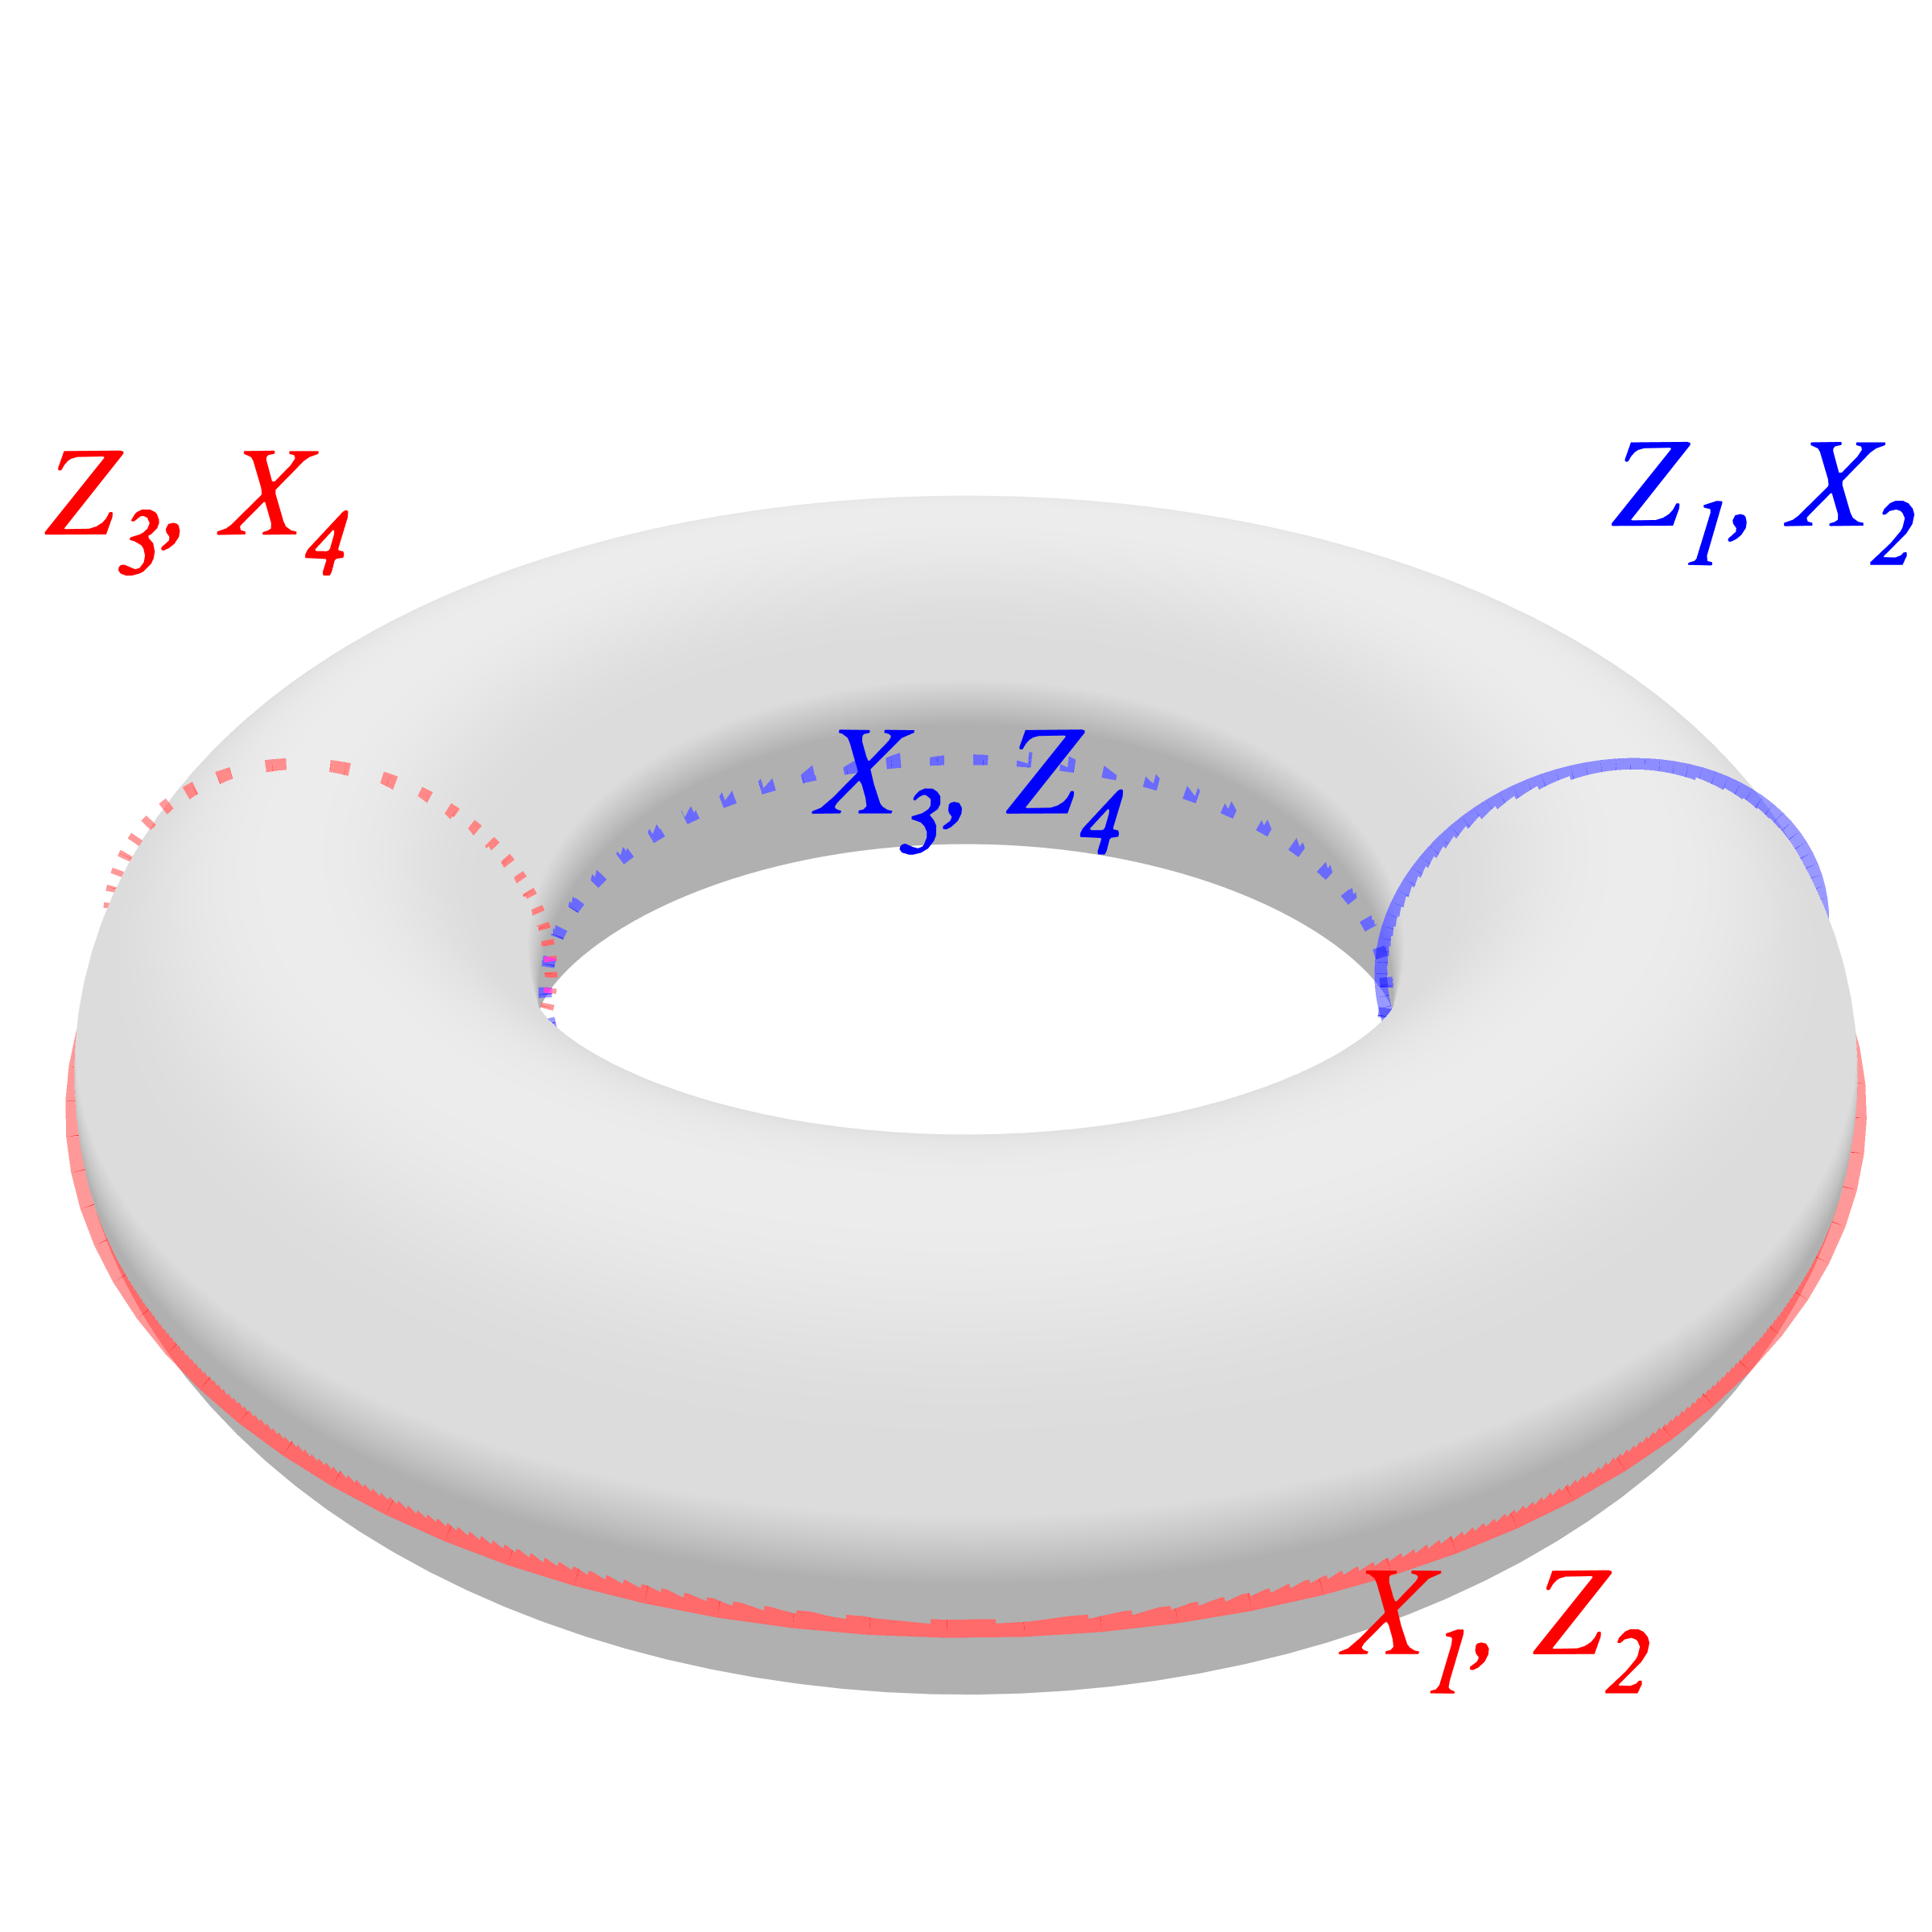
\includegraphics[width=0.85\linewidth]{figures/chapter_2/c2_torus_colorcode.png}
        \caption{}
    \end{subfigure}
    \hfill
    \begin{subfigure}[b]{0.345\textwidth}
        \centering
                \begin{tikzpicture}[scale=0.31]
            \def\L{1.3657} 
            \colorlet{colR}{red!20} \colorlet{colG}{green!20} \colorlet{colB}{blue!20}
            
            \colorlet{darkR}{red!75!black}
            \colorlet{lightR}{red}
            \colorlet{darkB}{blue!75!black}
            \colorlet{lightB}{cyan!80!blue}
            
            \newcommand{\sq}[3]{ \filldraw[fill=#3, draw=black, thick] ({#1-0.4},{#2-0.4}) rectangle ({#1+0.4},{#2+0.4}); }
            \newcommand{\oct}[3]{
                \filldraw[fill=#3, draw=black, thick]
                    ({#1-0.4},{#2-0.9657}) -- ({#1+0.4},{#2-0.9657}) -- ({#1+0.9657},{#2-0.4}) --
                    ({#1+0.9657},{#2+0.4}) -- ({#1+0.4},{#2+0.9657}) -- ({#1-0.4},{#2+0.9657}) --
                    ({#1-0.9657},{#2+0.4}) -- ({#1-0.9657},{#2-0.4}) -- cycle;
            }
    
            \begin{scope}
                \clip (-4.5, -4.5) rectangle (4.5, 4.5);
                
                \begin{scope}[rotate=45]
                    \foreach \i in {-7, -5, -3, -1, 1, 3, 5, 7} \foreach \j in {-6, -4, -2, 0, 2, 4, 6} \oct{\i*\L}{\j*\L}{colB};
                    \foreach \i in {-6, -4, -2, 0, 2, 4, 6} \foreach \j in {-7, -5, -3, -1, 1, 3, 5, 7} \oct{\i*\L}{\j*\L}{colG};
                    \foreach \i in {-6, -4, -2, 0, 2, 4, 6} \foreach \j in {-6, -4, -2, 0, 2, 4, 6} \sq{\i*\L}{\j*\L}{colR};
                    \foreach \i in {-7, -5, -3, -1, 1, 3, 5, 7} \foreach \j in {-7, -5, -3, -1, 1, 3, 5, 7} \sq{\i*\L}{\j*\L}{colR};
    
                    \foreach \k in {-3, -2, -1, 0, 1, 2, 3} {
                        \pgfmathparse{mod(abs(\k), 2) == 1 ? 1 : 0}
                        \ifnum\pgfmathresult=1
                            \draw[darkB, line width=1.5pt] ({\k*\L + 0.4}, {-\k*\L + 0.4}) -- ({\k*\L + 0.4}, {-\k*\L - 0.4});
                            \ifnum\k<3 \draw[darkB, densely dotted, line width=1.5pt] ({\k*\L + 0.4}, {-\k*\L - 0.4}) -- ({(\k+1)*\L - 0.4}, {-(\k+1)*\L - 0.4}); \fi
                        \else
                            \draw[darkB, line width=1.5pt] ({\k*\L - 0.4}, {-\k*\L - 0.4}) -- ({\k*\L + 0.4}, {-\k*\L - 0.4});
                            \ifnum\k<3 \draw[darkB, densely dotted, line width=1.5pt] ({\k*\L + 0.4}, {-\k*\L - 0.4}) -- ({(\k+1)*\L + 0.4}, {-(\k+1)*\L + 0.4}); \fi
                        \fi
                    }
        
                    \foreach \k in {-3, -2, -1, 0, 1, 2, 3} {
                        \pgfmathparse{mod(abs(\k), 2) == 1 ? 1 : 0}
                        \ifnum\pgfmathresult=1
                            \draw[lightB, line width=1.5pt] ({\k*\L + 0.4}, {\k*\L - 0.4}) -- ({\k*\L + 0.4}, {\k*\L + 0.4});
                            \ifnum\k<3 \draw[lightB, densely dotted, line width=1.5pt] ({\k*\L + 0.4}, {\k*\L + 0.4}) -- ({(\k+1)*\L - 0.4}, {(\k+1)*\L + 0.4}); \fi
                        \else
                            \draw[lightB, line width=1.5pt] ({\k*\L - 0.4}, {\k*\L + 0.4}) -- ({\k*\L + 0.4}, {\k*\L + 0.4});
                            \ifnum\k<3 \draw[lightB, densely dotted, line width=1.5pt] ({\k*\L + 0.4}, {\k*\L + 0.4}) -- ({(\k+1)*\L + 0.4}, {(\k+1)*\L - 0.4}); \fi
                        \fi
                    }
    
                    % Red Vertical (Desplazada hacia la izquierda)
                    \foreach \k in {-6, -5, -4, -3, -2, -1, 0, 1, 2, 3, 4, 5} {
                        \draw[darkR, line width=1.5pt] ({(\k-2)*\L + 0.4}, {\k*\L + 0.4}) -- ({(\k-1)*\L - 0.4}, {(\k+1)*\L - 0.4});
                        \draw[darkR, densely dotted, line width=1.5pt] ({(\k-1)*\L - 0.4}, {(\k+1)*\L - 0.4}) -- ({(\k-1)*\L}, {(\k+1)*\L}) -- ({(\k-1)*\L + 0.4}, {(\k+1)*\L + 0.4});
                    }

                    % Red Horizontal (Desplazada hacia abajo)
                    \foreach \k in {-6, -5, -4, -3, -2, -1, 0, 1, 2, 3, 4, 5} {
                        \draw[lightR, line width=1.5pt] ({\k*\L + 0.4}, {(-\k-2)*\L - 0.4}) -- ({(\k+1)*\L - 0.4}, {(-\k-3)*\L + 0.4});
                        \draw[lightR, densely dotted, line width=1.5pt] ({(\k+1)*\L - 0.4}, {(-\k-3)*\L + 0.4}) -- ({(\k+1)*\L}, {(-\k-3)*\L}) -- ({(\k+1)*\L + 0.4}, {(-\k-3)*\L - 0.4});
                    }

                    \foreach \k in {-3, -2, -1, 0, 1, 2, 3} {
                        \pgfmathparse{mod(abs(\k), 2) == 1 ? 1 : 0}
                        \ifnum\pgfmathresult=1
                            \filldraw[black, fill=white, thick] ({\k*\L + 0.4}, {-\k*\L + 0.4}) circle (2.5pt);
                            \filldraw[black, fill=white, thick] ({\k*\L + 0.4}, {-\k*\L - 0.4}) circle (2.5pt);
                            \filldraw[black, fill=white, thick] ({\k*\L + 0.4}, {\k*\L - 0.4}) circle (2.5pt);
                            \filldraw[black, fill=white, thick] ({\k*\L + 0.4}, {\k*\L + 0.4}) circle (2.5pt);
                        \else
                            \filldraw[black, fill=white, thick] ({\k*\L - 0.4}, {-\k*\L - 0.4}) circle (2.5pt);
                            \filldraw[black, fill=white, thick] ({\k*\L + 0.4}, {-\k*\L - 0.4}) circle (2.5pt);
                            \filldraw[black, fill=white, thick] ({\k*\L - 0.4}, {\k*\L + 0.4}) circle (2.5pt);
                            \filldraw[black, fill=white, thick] ({\k*\L + 0.4}, {\k*\L + 0.4}) circle (2.5pt);
                        \fi
                    }
                    
                    % Qubits de las cuerdas rojas también desplazados
                    \foreach \k in {-6, -5, -4, -3, -2, -1, 0, 1, 2, 3, 4, 5} {
                        \filldraw[black, fill=white, thick] ({(\k-2)*\L + 0.4}, {\k*\L + 0.4}) circle (2.5pt);
                        \filldraw[black, fill=white, thick] ({(\k-1)*\L - 0.4}, {(\k+1)*\L - 0.4}) circle (2.5pt);
                        \filldraw[black, fill=white, thick] ({\k*\L + 0.4}, {(-\k-2)*\L - 0.4}) circle (2.5pt);
                        \filldraw[black, fill=white, thick] ({(\k+1)*\L - 0.4}, {(-\k-3)*\L + 0.4}) circle (2.5pt);
                    }
                \end{scope}
            \end{scope}
    
            % Etiquetas de las líneas
            % Horizontal Blue (Azul oscura): Arriba, en el lado izquierdo
            \node[above, darkB, fill=white, fill opacity=0.7,text opacity=1, inner sep=1pt, rounded corners=2pt] at (3.0, 0.5) {$\mathbf{X_{L1}, Z_{L2}}$};
            
            % Horizontal Red (Roja clara): Debajo de su línea, en el lado izquierdo
            \node[below, lightR, fill=white, fill opacity=0.7,text opacity=1, inner sep=1pt, rounded corners=2pt] at (3.0, -1.93) {$\mathbf{Z_{L3}, X_{L4}}$};
            
            % Vertical Red (Roja oscura): A la derecha de su línea, en la parte de abajo
            \node[right, darkR, fill=white, fill opacity=0.7,text opacity=1, inner sep=1pt, rounded corners=2pt] at (-1.93, -4.0) {$\mathbf{X_{L3}, Z_{L4}}$};
            
            % Vertical Blue (Azul clara): Queda en el lado superior derecho como antes
            \node[right, lightB, fill=white, fill opacity=0.7,text opacity=1, inner sep=1pt, rounded corners=2pt] at (0, 3.5) {$\mathbf{Z_{L1}, X_{L2}}$};
            
        \end{tikzpicture}

        \caption{}
    \end{subfigure}
    \hfill
    \begin{subfigure}[b]{0.335\textwidth}
        \centering
                \begin{tikzpicture}[scale=0.295]
            \def\L{1.732}
            \colorlet{colR}{red!20} \colorlet{colG}{green!20} \colorlet{colB}{blue!20}
            
            \colorlet{darkR}{red!75!black}
            \colorlet{lightR}{red}
            \colorlet{darkB}{blue!75!black}
            \colorlet{lightB}{cyan!80!blue}
            
            \newcommand{\hex}[3]{
                \filldraw[fill=#3, draw=black, thick]
                    ({#1-1},{#2}) -- ({#1-0.5},{#2+0.866}) -- ({#1+0.5},{#2+0.866}) --
                    ({#1+1},{#2}) -- ({#1+0.5},{#2-0.866}) -- ({#1-0.5},{#2-0.866}) -- cycle;
            }

            \begin{scope}
                \clip (-4.5, -4.5) rectangle (4.5, 4.5);
                
                \foreach \u in {-4,...,4} {
                    \foreach \v in {-4,...,4} {
                        \pgfmathparse{int(mod(\u-\v+30, 3))}
                        \ifnum\pgfmathresult=0 \hex{1.5*\u}{0.866*\u + 1.732*\v}{colR} \fi
                        \ifnum\pgfmathresult=1 \hex{1.5*\u}{0.866*\u + 1.732*\v}{colG} \fi
                        \ifnum\pgfmathresult=2 \hex{1.5*\u}{0.866*\u + 1.732*\v}{colB} \fi
                    }
                }

                \foreach \k in {-2, -1, 0, 1, 2} {
                    \draw[darkB, densely dotted, line width=1.5pt] ({3*\k - 1}, 1.732) -- ({3*\k + 1}, 1.732);
                    \draw[darkB, line width=1.5pt] ({3*\k + 1}, 1.732) -- ({3*\k + 2}, 1.732);
                }

                \foreach \k in {-2, -1, 0, 1, 2} {
                    \draw[lightR, densely dotted, line width=1.5pt] ({3*\k - 1}, 0) -- ({3*\k + 1}, 0);
                    \draw[lightR, line width=1.5pt] ({3*\k + 1}, 0) -- ({3*\k + 2}, 0);
                }

                \foreach \k in {-2, -1, 0, 1, 2} {
                    \pgfmathparse{mod(abs(\k), 2) == 1 ? 1 : 0}
                    \ifnum\pgfmathresult=1
                        \draw[lightB, densely dotted, line width=1.5pt] (-0.5, {-1.732 + 2.598*\k}) -- (-0.5, {0 + 2.598*\k});
                        \draw[lightB, line width=1.5pt] (-0.5, {0 + 2.598*\k}) -- (-1.0, {0.866 + 2.598*\k});
                    \else
                        \draw[lightB, densely dotted, line width=1.5pt] (-1.0, {-1.732 + 2.598*\k}) -- (-1.0, {0 + 2.598*\k});
                        \draw[lightB, line width=1.5pt] (-1.0, {0 + 2.598*\k}) -- (-0.5, {0.866 + 2.598*\k});
                    \fi
                }

                \foreach \k in {-2, -1, 0, 1, 2} {
                    \pgfmathparse{mod(abs(\k), 2) == 1 ? 1 : 0}
                    \ifnum\pgfmathresult=1
                        \draw[darkR, densely dotted, line width=1.5pt] (1.0, {-0.866 + 2.598*\k}) -- (1.0, {0.866 + 2.598*\k});
                        \draw[darkR, line width=1.5pt] (1.0, {0.866 + 2.598*\k}) -- (0.5, {1.732 + 2.598*\k});
                    \else
                        \draw[darkR, densely dotted, line width=1.5pt] (0.5, {-0.866 + 2.598*\k}) -- (0.5, {0.866 + 2.598*\k});
                        \draw[darkR, line width=1.5pt] (0.5, {0.866 + 2.598*\k}) -- (1.0, {1.732 + 2.598*\k});
                    \fi
                }
                
                \foreach \k in {-2, -1, 0, 1, 2} {
                    \filldraw[black, fill=white, thick] ({3*\k - 1}, 1.732) circle (2.5pt);
                    \filldraw[black, fill=white, thick] ({3*\k + 1}, 1.732) circle (2.5pt);
                    \filldraw[black, fill=white, thick] ({3*\k + 2}, 1.732) circle (2.5pt);
                    
                    \filldraw[black, fill=white, thick] ({3*\k - 1}, 0) circle (2.5pt);
                    \filldraw[black, fill=white, thick] ({3*\k + 1}, 0) circle (2.5pt);
                    \filldraw[black, fill=white, thick] ({3*\k + 2}, 0) circle (2.5pt);
                    
                    \pgfmathparse{mod(abs(\k), 2) == 1 ? 1 : 0}
                    \ifnum\pgfmathresult=1
                        \filldraw[black, fill=white, thick] (-0.5, {-1.732 + 2.598*\k}) circle (2.5pt);
                        \filldraw[black, fill=white, thick] (-0.5, {0 + 2.598*\k}) circle (2.5pt);
                        \filldraw[black, fill=white, thick] (-1.0, {0.866 + 2.598*\k}) circle (2.5pt);
                    \else
                        \filldraw[black, fill=white, thick] (-1.0, {-1.732 + 2.598*\k}) circle (2.5pt);
                        \filldraw[black, fill=white, thick] (-1.0, {0 + 2.598*\k}) circle (2.5pt);
                        \filldraw[black, fill=white, thick] (-0.5, {0.866 + 2.598*\k}) circle (2.5pt);
                    \fi
                    
                    \pgfmathparse{mod(abs(\k), 2) == 1 ? 1 : 0}
                    \ifnum\pgfmathresult=1
                        \filldraw[black, fill=white, thick] (1.0, {-0.866 + 2.598*\k}) circle (2.5pt);
                        \filldraw[black, fill=white, thick] (1.0, {0.866 + 2.598*\k}) circle (2.5pt);
                        \filldraw[black, fill=white, thick] (0.5, {1.732 + 2.598*\k}) circle (2.5pt);
                    \else
                        \filldraw[black, fill=white, thick] (0.5, {-0.866 + 2.598*\k}) circle (2.5pt);
                        \filldraw[black, fill=white, thick] (0.5, {0.866 + 2.598*\k}) circle (2.5pt);
                        \filldraw[black, fill=white, thick] (1.0, {1.732 + 2.598*\k}) circle (2.5pt);
                    \fi
                }
            \end{scope}

            \node[above, darkB, fill=white, fill opacity=0.7,text opacity=1, inner sep=1pt, rounded corners=2pt] at (-3.5, 1.732) {$\mathbf{X_{L1}, Z_{L2}}$};
            \node[below, lightR, fill=white, fill opacity=0.7,text opacity=1, inner sep=1pt, rounded corners=2pt] at (3.5, 0) {$\mathbf{Z_{L3}, X_{L4}}$};
            
            \node[above, darkR, fill=white, fill opacity=0.7,text opacity=1, inner sep=1pt, rounded corners=2pt] at (2, 4.0) {$\mathbf{X_{L3}, Z_{L4}}$};
            \node[below, lightB, fill=white, fill opacity=0.7,text opacity=1, inner sep=1pt, rounded corners=2pt] at (-2, -4.0) {$\mathbf{Z_{L1}, X_{L2}}$};
            
        \end{tikzpicture}

        \caption{}
    \end{subfigure}

    \caption[Logical observables in a toric color code.]{Logical observables in a toric color code. \textbf{(a)} Logical observables correspond to color-independent non-contractible continuous strings wrapping around the two fundamental cycles of the torus. Color codes allow us to codify two logical operators in the same string, with the logical observables for each qubit being orthogonal. \textbf{(b)} The 4 independent strings in a $4.8.8$ lattice. \textbf{(c)} The 4 independent strings in a $6.6.6$ lattice.}
    \label{fig:2:color_code_logical_observables}
\end{figure}



In a color code, strings are \textit{colored}. A string can only be a border between faces of the other two colors, but it can go through faces of its color. For example, a "red" string of Pauli operators will strictly run along edges that separate green and blue faces, and will cross red faces. 

This color property leads to a unique topological feature: \textbf{string branching}. A string of one color can "unfold" or branch into two strings of the remaining colors at any vertex. For instance, a red string can split into a green string and a blue string, forming a structure known as a \textit{net}. This topological flexibility means that logical operators do not have to be simple linear loops; they can be complex, branching networks of operators that span the lattice.

These strings and nets define the logical operators. When two non-contractible nets of $X$ and $Z$ operators intersect at an odd number of data qubits, they anticommute, forming a valid logical qubit. Because of this rich combinatorial structure, a color code is twice as dense as a surface code. While a surface code wrapped on a torus natively encodes $k=2$ logical qubits, a color code on the exact same toroidal surface encodes $k=4$ logical qubits (see Figure \ref{fig:2:color_code_logical_observables}). For color codes planar implementations, triangular patches are typically used, which encode $k=1$ logical qubit but offer remarkably different boundary symmetries compared to the square patches of surface codes (see Figure \ref{fig:2:planar_color_code}). A square patch color code would encode $k=2$ logical qubits.

Despite the lattice being three-colorable and supporting strings of three distinct colors, only two of these colors are strictly independent from an error-correction perspective. In a 2D color code, every data qubit is located at a vertex shared by exactly three faces---one red, one green, and one blue. Consequently, any single error will always trigger a defect in exactly one face of each color. Because these syndrome defects are inherently created in triplets, the parity information gathered from any two colors fully determines the state of the third.

\subsection{Advantages: Transversality and 3D Topologies}
Color codes offer massive theoretical advantages over surface codes, primarily regarding logical gate execution. As discussed earlier in this chapter, finding transversal gates is highly desirable to prevent error propagation. 

Color codes natively possess a fully transversal Clifford gate set, meaning that critical operations like the Phase gate ($S$), Hadamard ($H$), and CNOT can be applied strictly pairwise, without the need for complex and noisy lattice surgery. 

\notatfm{Because of the Eastin-Knill Theorem, no QEC code can provide a universal set of transversal gates. Consequently, 3D color codes must sacrifice the transversal $H$ gate (which are easier to distill) in order to support a transversal $T$ gate. To circumvent this and achieve full universality without distillation, techniques like \textit{dimensional jumping} are employed. This allows the code to transition between 2D and 3D topologies, applying transversal $H$ gates while in the 2D configuration.} Furthermore, the color code topology can be generalized into three dimensions (3D). In 3D configurations, certain color codes allow the transversal execution of non-Clifford gates, such as the $T$-gate. This is a very significant advantage, as it bypasses the need for Magic State Distillation factories required by the surface code.

\subsection{Disadvantages and Processor Mapping}
Despite their theoretical superiority, 2D color codes face significant physical implementation hurdles. Their circuit-level threshold is generally lower than that of the surface code \cite{landahl2011fault}, meaning they require underlying hardware with significantly lower baseline noise to begin correcting errors effectively.

Moreover, the stabilizers acting on the faces involve a high number of qubits. For instance, in the 4.8.8 lattice, the octagonal faces represent weight-8 parity checks. Measuring a weight-8 stabilizer dynamically without exposing the data to correlated errors is a mapping challenge on modern hardware, which typically features restricted 2D grid connectivity.

Implementing these codes on real processors requires highly optimized, specialized layouts. For the \textbf{4.8.8 lattice}, Fowler \cite{Fowler_2011} demonstrated that it is possible to map this topology onto a standard 2D square architecture, although it requires replacing the ancilla qubit in octogonal faces with 5 ancilla qubits, 4 of them connected to two data qubits each, and the fifth one connected to the 4 ancilla qubits ((see Figure \ref{fig:2:planar_color_code})).


\begin{figure}[htbp]
    \centering
    \begin{subfigure}[b]{0.47\textwidth}
        \centering
        \input{figures/2.state_of_the_art/2-planar_color_code_a.tex}
        \caption{}
    \end{subfigure}
    \hfill
    \begin{subfigure}[b]{0.47\textwidth}
        \centering
                \begin{tikzpicture}[scale=0.45]
            \pgfdeclarelayer{background}
            \pgfsetlayers{background,main}
            \def\L{1.3657} 
            \colorlet{colR}{red!20} \colorlet{colG}{green!20} \colorlet{colB}{blue!20}
            
            \newcommand{\fullsq}[2]{
                \filldraw[fill=colR, draw=black, thick] ({#1-0.4},{#2-0.4}) rectangle ({#1+0.4},{#2+0.4});
                \draw[black!60, thick] ({#1},{#2}) -- ({#1-0.4},{#2-0.4});
                \draw[black!60, thick] ({#1},{#2}) -- ({#1+0.4},{#2-0.4});
                \draw[black!60, thick] ({#1},{#2}) -- ({#1-0.4},{#2+0.4});
                \draw[black!60, thick] ({#1},{#2}) -- ({#1+0.4},{#2+0.4});
                \filldraw[black] ({#1},{#2}) circle (1.5pt);
            }
            
            \newcommand{\fulloct}[3]{
                \filldraw[fill=#3, draw=black, thick]
                    ({#1-0.4},{#2-0.9657}) -- ({#1+0.4},{#2-0.9657}) -- ({#1+0.9657},{#2-0.4}) --
                    ({#1+0.9657},{#2+0.4}) -- ({#1+0.4},{#2+0.9657}) -- ({#1-0.4},{#2+0.9657}) --
                    ({#1-0.9657},{#2+0.4}) -- ({#1-0.9657},{#2-0.4}) -- cycle;
                \def\off{0.4}
                \draw[black!60, thick] ({#1},{#2}) -- ({#1+\off},{#2+\off});
                \draw[black!60, thick] ({#1},{#2}) -- ({#1+\off},{#2-\off});
                \draw[black!60, thick] ({#1},{#2}) -- ({#1-\off},{#2-\off});
                \draw[black!60, thick] ({#1},{#2}) -- ({#1-\off},{#2+\off});
                \draw[black!60, thick] ({#1+\off},{#2+\off}) -- ({#1+0.4},{#2+0.9657});
                \draw[black!60, thick] ({#1+\off},{#2+\off}) -- ({#1+0.9657},{#2+0.4});
                \draw[black!60, thick] ({#1+\off},{#2-\off}) -- ({#1+0.9657},{#2-0.4});
                \draw[black!60, thick] ({#1+\off},{#2-\off}) -- ({#1+0.4},{#2-0.9657});
                \draw[black!60, thick] ({#1-\off},{#2-\off}) -- ({#1-0.4},{#2-0.9657});
                \draw[black!60, thick] ({#1-\off},{#2-\off}) -- ({#1-0.9657},{#2-0.4});
                \draw[black!60, thick] ({#1-\off},{#2+\off}) -- ({#1-0.9657},{#2+0.4});
                \draw[black!60, thick] ({#1-\off},{#2+\off}) -- ({#1-0.4},{#2+0.9657});
                \filldraw[black] ({#1+\off},{#2+\off}) circle (1.5pt);
                \filldraw[black] ({#1+\off},{#2-\off}) circle (1.5pt);
                \filldraw[black] ({#1-\off},{#2-\off}) circle (1.5pt);
                \filldraw[black] ({#1-\off},{#2+\off}) circle (1.5pt);
                \filldraw[black] ({#1},{#2}) circle (1.5pt);
            }
    
            \newcommand{\trapBtop}[2]{
                \filldraw[fill=colB, draw=black, thick]
                    ({#1-0.9657},{#2+0.4}) -- ({#1-0.4},{#2+0.9657}) -- 
                    ({#1+0.4},{#2+0.9657}) -- ({#1+0.9657},{#2+0.4}) -- cycle;
                \def\ancY{#2+0.68}
                \draw[black!60, thick] ({#1},{\ancY}) -- ({#1-0.9657},{#2+0.4});
                \draw[black!60, thick] ({#1},{\ancY}) -- ({#1-0.4},{#2+0.9657});
                \draw[black!60, thick] ({#1},{\ancY}) -- ({#1+0.4},{#2+0.9657});
                \draw[black!60, thick] ({#1},{\ancY}) -- ({#1+0.9657},{#2+0.4});
                \filldraw[black] ({#1},{\ancY}) circle (1.5pt);
            }
    
            \newcommand{\trapBright}[2]{
                \filldraw[fill=colB, draw=black, thick]
                    ({#1+0.9657},{#2+0.4}) -- ({#1+0.9657},{#2-0.4}) -- 
                    ({#1+0.4},{#2-0.9657}) -- ({#1-0.4},{#2-0.9657}) -- cycle;
                \def\ancX{#1+0.48}
                \def\ancY{#2-0.48}
                \draw[black!60, thick] ({\ancX},{\ancY}) -- ({#1+0.9657},{#2+0.4});
                \draw[black!60, thick] ({\ancX},{\ancY}) -- ({#1+0.9657},{#2-0.4});
                \draw[black!60, thick] ({\ancX},{\ancY}) -- ({#1+0.4},{#2-0.9657});
                \draw[black!60, thick] ({\ancX},{\ancY}) -- ({#1-0.4},{#2-0.9657});
                \filldraw[black] ({\ancX},{\ancY}) circle (1.5pt);
            }
            
            \newcommand{\trapGleft}[2]{
                \filldraw[fill=colG, draw=black, thick]
                    ({#1-0.9657},{#2+0.4}) -- ({#1-0.9657},{#2-0.4}) -- 
                    ({#1-0.4},{#2-0.9657}) -- ({#1+0.4},{#2-0.9657}) -- cycle;
                \def\ancX{#1-0.48}
                \def\ancY{#2-0.48}
                \draw[black!60, thick] ({\ancX},{\ancY}) -- ({#1-0.9657},{#2+0.4});
                \draw[black!60, thick] ({\ancX},{\ancY}) -- ({#1-0.9657},{#2-0.4});
                \draw[black!60, thick] ({\ancX},{\ancY}) -- ({#1-0.4},{#2-0.9657});
                \draw[black!60, thick] ({\ancX},{\ancY}) -- ({#1+0.4},{#2-0.9657});
                \filldraw[black] ({\ancX},{\ancY}) circle (1.5pt);
            }
    
            \newcommand{\fullsqqubits}[2]{
                \filldraw[fill=white, draw=black, thick] ({#1-0.4},{#2-0.4}) circle (2.5pt);
                \filldraw[fill=white, draw=black, thick] ({#1+0.4},{#2-0.4}) circle (2.5pt);
                \filldraw[fill=white, draw=black, thick] ({#1+0.4},{#2+0.4}) circle (2.5pt);
                \filldraw[fill=white, draw=black, thick] ({#1-0.4},{#2+0.4}) circle (2.5pt);
            }
            
            \newcommand{\fulloctqubits}[2]{
                \filldraw[fill=white, draw=black, thick] ({#1-0.4},{#2-0.9657}) circle (2.5pt);
                \filldraw[fill=white, draw=black, thick] ({#1+0.4},{#2-0.9657}) circle (2.5pt);
                \filldraw[fill=white, draw=black, thick] ({#1+0.9657},{#2-0.4}) circle (2.5pt);
                \filldraw[fill=white, draw=black, thick] ({#1+0.9657},{#2+0.4}) circle (2.5pt);
                \filldraw[fill=white, draw=black, thick] ({#1+0.4},{#2+0.9657}) circle (2.5pt);
                \filldraw[fill=white, draw=black, thick] ({#1-0.4},{#2+0.9657}) circle (2.5pt);
                \filldraw[fill=white, draw=black, thick] ({#1-0.9657},{#2+0.4}) circle (2.5pt);
                \filldraw[fill=white, draw=black, thick] ({#1-0.9657},{#2-0.4}) circle (2.5pt);
            }
            
            \newcommand{\trapBtopqubits}[2]{
                \filldraw[fill=white, draw=black, thick] ({#1-0.9657},{#2+0.4}) circle (2.5pt);
                \filldraw[fill=white, draw=black, thick] ({#1-0.4},{#2+0.9657}) circle (2.5pt);
                \filldraw[fill=white, draw=black, thick] ({#1+0.4},{#2+0.9657}) circle (2.5pt);
                \filldraw[fill=white, draw=black, thick] ({#1+0.9657},{#2+0.4}) circle (2.5pt);
            }
            
            \newcommand{\trapBrightqubits}[2]{
                \filldraw[fill=white, draw=black, thick] ({#1+0.9657},{#2+0.4}) circle (2.5pt);
                \filldraw[fill=white, draw=black, thick] ({#1+0.9657},{#2-0.4}) circle (2.5pt);
                \filldraw[fill=white, draw=black, thick] ({#1+0.4},{#2-0.9657}) circle (2.5pt);
                \filldraw[fill=white, draw=black, thick] ({#1-0.4},{#2-0.9657}) circle (2.5pt);
            }
            
            \newcommand{\trapGleftqubits}[2]{
                \filldraw[fill=white, draw=black, thick] ({#1-0.9657},{#2+0.4}) circle (2.5pt);
                \filldraw[fill=white, draw=black, thick] ({#1-0.9657},{#2-0.4}) circle (2.5pt);
                \filldraw[fill=white, draw=black, thick] ({#1-0.4},{#2-0.9657}) circle (2.5pt);
                \filldraw[fill=white, draw=black, thick] ({#1+0.4},{#2-0.9657}) circle (2.5pt);
            }
    
            \trapBtop{-3*\L}{0}
            \trapBtop{-\L}{0}
            \trapBtop{\L}{0}
            \trapBtop{3*\L}{0}
    
            \fullsq{-3*\L}{\L}
            \fulloct{-2*\L}{\L}{colG}
            \fullsq{-\L}{\L}
            \fulloct{0}{\L}{colG}
            \fullsq{\L}{\L}
            \fulloct{2*\L}{\L}{colG}
            \fullsq{3*\L}{\L}
            \trapGleft{4*\L}{\L}
    
            \trapBright{-3*\L}{2*\L}
            \fullsq{-2*\L}{2*\L}
            \fulloct{-\L}{2*\L}{colB}
            \fullsq{0}{2*\L}
            \fulloct{\L}{2*\L}{colB}
            \fullsq{2*\L}{2*\L}
    
            \fullsq{-\L}{3*\L}
            \fulloct{0}{3*\L}{colG}
            \fullsq{\L}{3*\L}
            \trapGleft{2*\L}{3*\L}
    
            \trapBright{-\L}{4*\L}
            \fullsq{0}{4*\L}
    
            \trapBtopqubits{-3*\L}{0}
            \trapBtopqubits{-\L}{0}
            \trapBtopqubits{\L}{0}
            \trapBtopqubits{3*\L}{0}
    
            \fullsqqubits{-3*\L}{\L}
            \fulloctqubits{-2*\L}{\L}
            \fullsqqubits{-\L}{\L}
            \fulloctqubits{0}{\L}
            \fullsqqubits{\L}{\L}
            \fulloctqubits{2*\L}{\L}
            \fullsqqubits{3*\L}{\L}
            \trapGleftqubits{4*\L}{\L}
    
            \trapBrightqubits{-3*\L}{2*\L}
            \fullsqqubits{-2*\L}{2*\L}
            \fulloctqubits{-\L}{2*\L}
            \fullsqqubits{0}{2*\L}
            \fulloctqubits{\L}{2*\L}
            \fullsqqubits{2*\L}{2*\L}
    
            \fullsqqubits{-\L}{3*\L}
            \fulloctqubits{0}{3*\L}
            \fullsqqubits{\L}{3*\L}
            \trapGleftqubits{2*\L}{3*\L}
    
            \trapBrightqubits{-\L}{4*\L}
            \fullsqqubits{0}{4*\L}
    
            \begin{pgfonlayer}{background}
                \draw[red, line width=4pt, line cap=round] 
                    ({-3*\L-0.9657}, 0.4) -- ({4*\L+0.4}, 0.4);
    
                \draw[green!60!black, line width=4pt, rounded corners=1pt, line cap=round]
                    ({-3*\L-0.9657}, 0.4) 
                    -- ({-3*\L-0.4}, 0.9657)
                    -- ({-3*\L-0.4}, {\L+0.4})
                    -- ({-2*\L-0.4}, {2*\L+0.4})
                    -- ({-2*\L+0.4}, {2*\L+0.4})
                    -- ({-\L-0.4}, {3*\L-0.4})
                    -- ({-\L-0.4}, {3*\L+0.4})
                    -- ({-0.4}, {4*\L+0.4})
                    -- ({0.4}, {4*\L+0.4});
    
                \draw[blue, line width=4pt, rounded corners=1pt, line cap=round]
                    ({4*\L+0.4}, 0.4)
                    -- ({3*\L+0.4}, {\L+0.4})
                    -- ({3*\L-0.4}, {\L+0.4})
                    -- ({2*\L+0.4}, {2*\L-0.4})
                    -- ({2*\L+0.4}, {2*\L+0.4})
                    -- ({\L+0.4}, {3*\L+0.4})
                    -- ({\L-0.4}, {3*\L+0.4})
                    -- ({0.4}, {4*\L-0.4})
                    -- ({0.4}, {4*\L+0.4});
            \end{pgfonlayer}
        \end{tikzpicture}

        \caption{}
    \end{subfigure}
    \caption[Planar topology of a 4.8.8 lattice color code.]{Planar topology of a 4.8.8 lattice color code. \textbf{(a)} Definition of the triangular patch for a planar topology, in which we must use string-nets to define the logical observables. Each string-net can encode the logical $X$ and $Z$ operators in the color code, but the individual strings must terminate at a boundary of their own color, which inherently requires branching. \textbf{(b)} Mapping of the color code patch to a quantum processor with a square grid of qubits. For the octagonal faces, we must use 5 ancillas to perform the stabilizer measurements. Ancilla qubits in the tetrahedrons that appear in the boundaries do not map the square grid and are intentionally simplified in this diagram.}
    \label{fig:2:planar_color_code}
\end{figure}


Similarly, the \textbf{6.6.6 hexagonal lattice} maps naturally to certain architectures, but it is still a non-trivial problem. Recent publications by Lacroix et al. \cite{Lacroix_2025} outline an optimized mapping for the 6.6.6 code.

\section{Non-topological QLDPC Codes}

\notatfm{The BPT bound mathematically proves that for any quantum code restricted to local interactions in 2D, the parameters must satisfy $k d^2 \leq O(n)$. This implies that the physical overhead per logical qubit ($n/k$) must grow at least as $d^2$. If higher error protection is needed (higher $d$), the physical footprint explodes quadratically.} While 2D topological codes are very hardware-friendly, their reliance on local 2D planes strictly limits their scalability. The fundamental bottleneck of local 2D codes is governed by the Bravyi-Poulin-Terhal (BPT) bound \cite{Bravyi_2010}. To build future quantum supercomputers with millions of qubits and increasing distances for longer computations, this geometric restriction imposes a prohibitive physical overhead.

This fact has drawn massive attention to non-topological Quantum Low-Density Parity-Check (QLDPC) codes. By sacrificing strictly local 2D connectivity and embracing long-range physical connections, these codes break the BPT bound. In a topological code, increasing the distance requires making the 2D patch larger, which squares the number of physical qubits. QLDPC codes, instead, can maintain a constant encoding rate while the distance grows linearly with the number of physical qubits. This removes the quadratic penalty for fault tolerance.

\subsection{Bivariate Bicycle Codes (BBC)}

A prominent recent breakthrough in the practical domain is the Bivariate Bicycle Code (BBC) family, introduced by Bravyi et al. \cite{bravyi2024high}. These codes prove that we can encode dozens of logical qubits with high distances using only a fraction of the physical qubits required by topological codes. In 2D topological codes like the Surface Code, the number of physical qubits $n$ scales quadratically with the distance ($n \propto d^2$), which means that encoding $k$ logical qubits requires scaling the hardware footprint dramatically as $O(k d^2)$. Non-topological QLDPC codes, and specifically BBCs, achieve a constant encoding rate $k/n \sim \text{const}$, meaning they scale linearly: the distance grows linearly with the number of physical qubits, bypassing the quadratic penalty.

To understand the massive savings: a typical BBC presented in \cite{bravyi2024high} encodes $k=12$ logical qubits with a distance of $d=12$ using $n=144$ data qubits (and $144$ ancillas, totaling $288$ physical qubits). To achieve the exact same protection and capacity ($k=12, d=12$) using standard surface codes, one would need roughly $12 \times (12^2 + 12^2) = 3456$ physical qubits. This represents more than a $10\times$ reduction in hardware footprint.

The core ingenuity of BBCs lies in how they guarantee that $X$-type and $Z$-type stabilizers commute, which is the most difficult challenge when designing any quantum code. In the stabilizer formalism, an $X$-stabilizer and a $Z$-stabilizer commute if and only if they overlap on an even number of physical qubits. 

\notatfm{A \textbf{parity check matrix} is a mathematical representation of the stabilizer group. In this matrix, each row represents a single stabilizer generator (a parity check) and each column represents a physical data qubit. A $1$ at position $(i, j)$ means that the $i$-th check operator acts on the $j$-th qubit.}Instead of trying to manually guess which qubits to connect to satisfy this rule, BBCs use a clever mathematical trick. The physical data qubits are divided into two equal groups (the two "bicycles", typically referred to as the Left and Right blocks). Each block is mathematically treated as a virtual 2D grid of dimensions $\ell \times m$ (rows and columns), containing $\ell \cdot m$ qubits. The parity check matrices are then constructed using two commutative matrices, $A$ and $B$, which are derived from polynomials with two variables, $x$ and $y$. The $X$-type parity check matrix is defined as $H^X = [A \mid B]$, and the $Z$-type parity check matrix is defined as $H^Z = [B^T \mid A^T]$.

Because the matrices $A$ and $B$ are built from commutative polynomials, they commute ($AB = BA$). When computing the overlap between $X$ and $Z$ checks, the mathematical structure yields $H^X (H^Z)^T = AB + BA$, which trivially equals $0 \pmod 2$. This elegantly and automatically guarantees that any $X$-stabilizer and $Z$-stabilizer will always intersect on an even number of qubits, ensuring commutation without manual tweaking.

Physically, the variables $x$ and $y$ in the polynomials simply represent cyclic geometric shifts: $x$ acts as an instruction to "shift one position to the right" and $y$ means "shift one position down" on a virtual grid. A polynomial like $A = 1 + x + y^2$ acts as a wiring instruction that tells the hardware: "to build this stabilizer, apply the operator to a given qubit ($1$), the qubit to its right ($x$), and the qubit two steps down ($y^2$)". 

By keeping these "wiring instructions" very short (e.g., using exactly three terms for $A$ and three terms for $B$), the total weight of every parity check is strictly bounded to exactly $3+3=6$ qubits, regardless of how large the total code (the grid) becomes. This naturally fulfills the Low-Density Parity-Check (LDPC) requirement, which is essential to prevent error propagation during syndrome measurements.

\begin{figure}[htpb!]
    \centering
    \resizebox{0.8\textwidth}{!}{
        \begin{tikzpicture}[scale=0.6, every node/.style={font=\sffamily}]
    % Define colors
    \colorlet{colL}{blue!40}
    \colorlet{colR}{orange!50}
    \colorlet{colX}{red!50}
    \colorlet{colZ}{green!50}
    \colorlet{colGrayFill}{gray!20}
    \colorlet{colGrayDraw}{gray!50}

\begin{scope}[shift={(0, 0)}]
  \node[anchor=south, font=\bfseries\large] at (8, 14.5) {Left Block Periodic Connections};
  \clip (3, 3) rectangle (14, 14);
  % Nodes
  \node[draw=colGrayDraw, fill=colGrayFill, circle, minimum size=0.45cm, inner sep=0pt] (L-0-0) at (0, 0) {};
  \node[draw=colGrayDraw, fill=colGrayFill, circle, minimum size=0.45cm, inner sep=0pt] (R-0-0) at (1, 1) {};
  \node[draw=colGrayDraw, fill=colGrayFill, regular polygon, regular polygon sides=4, minimum size=0.55cm, inner sep=0pt] (X-0-0) at (1, 0) {};
  \node[draw=colGrayDraw, fill=colGrayFill, regular polygon, regular polygon sides=4, minimum size=0.55cm, inner sep=0pt] (Z-0-0) at (0, 1) {};
  \node[draw=colGrayDraw, fill=colGrayFill, circle, minimum size=0.45cm, inner sep=0pt] (L-0-1) at (0, 2) {};
  \node[draw=colGrayDraw, fill=colGrayFill, circle, minimum size=0.45cm, inner sep=0pt] (R-0-1) at (1, 3) {};
  \node[draw=colGrayDraw, fill=colGrayFill, regular polygon, regular polygon sides=4, minimum size=0.55cm, inner sep=0pt] (X-0-1) at (1, 2) {};
  \node[draw=colGrayDraw, fill=colGrayFill, regular polygon, regular polygon sides=4, minimum size=0.55cm, inner sep=0pt] (Z-0-1) at (0, 3) {};
  \node[draw=colGrayDraw, fill=colGrayFill, circle, minimum size=0.45cm, inner sep=0pt] (L-0-2) at (0, 4) {};
  \node[draw=colGrayDraw, fill=colGrayFill, circle, minimum size=0.45cm, inner sep=0pt] (R-0-2) at (1, 5) {};
  \node[draw=colGrayDraw, fill=colGrayFill, regular polygon, regular polygon sides=4, minimum size=0.55cm, inner sep=0pt] (X-0-2) at (1, 4) {};
  \node[draw=colGrayDraw, fill=colGrayFill, regular polygon, regular polygon sides=4, minimum size=0.55cm, inner sep=0pt] (Z-0-2) at (0, 5) {};
  \node[draw=colGrayDraw, fill=colGrayFill, circle, minimum size=0.45cm, inner sep=0pt] (L-0-3) at (0, 6) {};
  \node[draw=colGrayDraw, fill=colGrayFill, circle, minimum size=0.45cm, inner sep=0pt] (R-0-3) at (1, 7) {};
  \node[draw=colGrayDraw, fill=colGrayFill, regular polygon, regular polygon sides=4, minimum size=0.55cm, inner sep=0pt] (X-0-3) at (1, 6) {};
  \node[draw=colGrayDraw, fill=colGrayFill, regular polygon, regular polygon sides=4, minimum size=0.55cm, inner sep=0pt] (Z-0-3) at (0, 7) {};
  \node[draw=colGrayDraw, fill=colGrayFill, circle, minimum size=0.45cm, inner sep=0pt] (L-0-4) at (0, 8) {};
  \node[draw=colGrayDraw, fill=colGrayFill, circle, minimum size=0.45cm, inner sep=0pt] (R-0-4) at (1, 9) {};
  \node[draw=colGrayDraw, fill=colGrayFill, regular polygon, regular polygon sides=4, minimum size=0.55cm, inner sep=0pt] (X-0-4) at (1, 8) {};
  \node[draw=colGrayDraw, fill=colGrayFill, regular polygon, regular polygon sides=4, minimum size=0.55cm, inner sep=0pt] (Z-0-4) at (0, 9) {};
  \node[draw=colGrayDraw, fill=colGrayFill, circle, minimum size=0.45cm, inner sep=0pt] (L-0-5) at (0, 10) {};
  \node[draw=colGrayDraw, fill=colGrayFill, circle, minimum size=0.45cm, inner sep=0pt] (R-0-5) at (1, 11) {};
  \node[draw=colGrayDraw, fill=colGrayFill, regular polygon, regular polygon sides=4, minimum size=0.55cm, inner sep=0pt] (X-0-5) at (1, 10) {};
  \node[draw=colGrayDraw, fill=colGrayFill, regular polygon, regular polygon sides=4, minimum size=0.55cm, inner sep=0pt] (Z-0-5) at (0, 11) {};
  \node[draw=colGrayDraw, fill=colGrayFill, circle, minimum size=0.45cm, inner sep=0pt] (L-0-6) at (0, 12) {};
  \node[draw=colGrayDraw, fill=colGrayFill, circle, minimum size=0.45cm, inner sep=0pt] (R-0-6) at (1, 13) {};
  \node[draw=colGrayDraw, fill=colGrayFill, regular polygon, regular polygon sides=4, minimum size=0.55cm, inner sep=0pt] (X-0-6) at (1, 12) {};
  \node[draw=colGrayDraw, fill=colGrayFill, regular polygon, regular polygon sides=4, minimum size=0.55cm, inner sep=0pt] (Z-0-6) at (0, 13) {};
  \node[draw=colGrayDraw, fill=colGrayFill, circle, minimum size=0.45cm, inner sep=0pt] (L-0-7) at (0, 14) {};
  \node[draw=colGrayDraw, fill=colGrayFill, circle, minimum size=0.45cm, inner sep=0pt] (R-0-7) at (1, 15) {};
  \node[draw=colGrayDraw, fill=colGrayFill, regular polygon, regular polygon sides=4, minimum size=0.55cm, inner sep=0pt] (X-0-7) at (1, 14) {};
  \node[draw=colGrayDraw, fill=colGrayFill, regular polygon, regular polygon sides=4, minimum size=0.55cm, inner sep=0pt] (Z-0-7) at (0, 15) {};
  \node[draw=colGrayDraw, fill=colGrayFill, circle, minimum size=0.45cm, inner sep=0pt] (L-0-8) at (0, 16) {};
  \node[draw=colGrayDraw, fill=colGrayFill, circle, minimum size=0.45cm, inner sep=0pt] (R-0-8) at (1, 17) {};
  \node[draw=colGrayDraw, fill=colGrayFill, regular polygon, regular polygon sides=4, minimum size=0.55cm, inner sep=0pt] (X-0-8) at (1, 16) {};
  \node[draw=colGrayDraw, fill=colGrayFill, regular polygon, regular polygon sides=4, minimum size=0.55cm, inner sep=0pt] (Z-0-8) at (0, 17) {};
  \node[draw=colGrayDraw, fill=colGrayFill, circle, minimum size=0.45cm, inner sep=0pt] (L-1-0) at (2, 0) {};
  \node[draw=colGrayDraw, fill=colGrayFill, circle, minimum size=0.45cm, inner sep=0pt] (R-1-0) at (3, 1) {};
  \node[draw=colGrayDraw, fill=colGrayFill, regular polygon, regular polygon sides=4, minimum size=0.55cm, inner sep=0pt] (X-1-0) at (3, 0) {};
  \node[draw=colGrayDraw, fill=colGrayFill, regular polygon, regular polygon sides=4, minimum size=0.55cm, inner sep=0pt] (Z-1-0) at (2, 1) {};
  \node[draw=colGrayDraw, fill=colGrayFill, circle, minimum size=0.45cm, inner sep=0pt] (L-1-1) at (2, 2) {};
  \node[draw=colGrayDraw, fill=colGrayFill, circle, minimum size=0.45cm, inner sep=0pt] (R-1-1) at (3, 3) {};
  \node[draw=colGrayDraw, fill=colGrayFill, regular polygon, regular polygon sides=4, minimum size=0.55cm, inner sep=0pt] (X-1-1) at (3, 2) {};
  \node[draw=colGrayDraw, fill=colGrayFill, regular polygon, regular polygon sides=4, minimum size=0.55cm, inner sep=0pt] (Z-1-1) at (2, 3) {};
  \node[draw=colGrayDraw, fill=colGrayFill, circle, minimum size=0.45cm, inner sep=0pt] (L-1-2) at (2, 4) {};
  \node[draw=colGrayDraw, fill=colGrayFill, circle, minimum size=0.45cm, inner sep=0pt] (R-1-2) at (3, 5) {};
  \node[draw=colGrayDraw, fill=colGrayFill, regular polygon, regular polygon sides=4, minimum size=0.55cm, inner sep=0pt] (X-1-2) at (3, 4) {};
  \node[draw=colGrayDraw, fill=colGrayFill, regular polygon, regular polygon sides=4, minimum size=0.55cm, inner sep=0pt] (Z-1-2) at (2, 5) {};
  \node[draw=colGrayDraw, fill=colGrayFill, circle, minimum size=0.45cm, inner sep=0pt] (L-1-3) at (2, 6) {};
  \node[draw=colGrayDraw, fill=colGrayFill, circle, minimum size=0.45cm, inner sep=0pt] (R-1-3) at (3, 7) {};
  \node[draw=colGrayDraw, fill=colGrayFill, regular polygon, regular polygon sides=4, minimum size=0.55cm, inner sep=0pt] (X-1-3) at (3, 6) {};
  \node[draw=colGrayDraw, fill=colGrayFill, regular polygon, regular polygon sides=4, minimum size=0.55cm, inner sep=0pt] (Z-1-3) at (2, 7) {};
  \node[draw=colGrayDraw, fill=colGrayFill, circle, minimum size=0.45cm, inner sep=0pt] (L-1-4) at (2, 8) {};
  \node[draw=colGrayDraw, fill=colGrayFill, circle, minimum size=0.45cm, inner sep=0pt] (R-1-4) at (3, 9) {};
  \node[draw=colGrayDraw, fill=colGrayFill, regular polygon, regular polygon sides=4, minimum size=0.55cm, inner sep=0pt] (X-1-4) at (3, 8) {};
  \node[draw=colGrayDraw, fill=colGrayFill, regular polygon, regular polygon sides=4, minimum size=0.55cm, inner sep=0pt] (Z-1-4) at (2, 9) {};
  \node[draw=colGrayDraw, fill=colGrayFill, circle, minimum size=0.45cm, inner sep=0pt] (L-1-5) at (2, 10) {};
  \node[draw=colGrayDraw, fill=colGrayFill, circle, minimum size=0.45cm, inner sep=0pt] (R-1-5) at (3, 11) {};
  \node[draw=colGrayDraw, fill=colGrayFill, regular polygon, regular polygon sides=4, minimum size=0.55cm, inner sep=0pt] (X-1-5) at (3, 10) {};
  \node[draw=colGrayDraw, fill=colGrayFill, regular polygon, regular polygon sides=4, minimum size=0.55cm, inner sep=0pt] (Z-1-5) at (2, 11) {};
  \node[draw=colGrayDraw, fill=colGrayFill, circle, minimum size=0.45cm, inner sep=0pt] (L-1-6) at (2, 12) {};
  \node[draw=colGrayDraw, fill=colGrayFill, circle, minimum size=0.45cm, inner sep=0pt] (R-1-6) at (3, 13) {};
  \node[draw=colGrayDraw, fill=colGrayFill, regular polygon, regular polygon sides=4, minimum size=0.55cm, inner sep=0pt] (X-1-6) at (3, 12) {};
  \node[draw=colGrayDraw, fill=colGrayFill, regular polygon, regular polygon sides=4, minimum size=0.55cm, inner sep=0pt] (Z-1-6) at (2, 13) {};
  \node[draw=colGrayDraw, fill=colGrayFill, circle, minimum size=0.45cm, inner sep=0pt] (L-1-7) at (2, 14) {};
  \node[draw=colGrayDraw, fill=colGrayFill, circle, minimum size=0.45cm, inner sep=0pt] (R-1-7) at (3, 15) {};
  \node[draw=colGrayDraw, fill=colGrayFill, regular polygon, regular polygon sides=4, minimum size=0.55cm, inner sep=0pt] (X-1-7) at (3, 14) {};
  \node[draw=colGrayDraw, fill=colGrayFill, regular polygon, regular polygon sides=4, minimum size=0.55cm, inner sep=0pt] (Z-1-7) at (2, 15) {};
  \node[draw=colGrayDraw, fill=colGrayFill, circle, minimum size=0.45cm, inner sep=0pt] (L-1-8) at (2, 16) {};
  \node[draw=colGrayDraw, fill=colGrayFill, circle, minimum size=0.45cm, inner sep=0pt] (R-1-8) at (3, 17) {};
  \node[draw=colGrayDraw, fill=colGrayFill, regular polygon, regular polygon sides=4, minimum size=0.55cm, inner sep=0pt] (X-1-8) at (3, 16) {};
  \node[draw=colGrayDraw, fill=colGrayFill, regular polygon, regular polygon sides=4, minimum size=0.55cm, inner sep=0pt] (Z-1-8) at (2, 17) {};
  \node[draw=colGrayDraw, fill=colGrayFill, circle, minimum size=0.45cm, inner sep=0pt] (L-2-0) at (4, 0) {};
  \node[draw=colGrayDraw, fill=colGrayFill, circle, minimum size=0.45cm, inner sep=0pt] (R-2-0) at (5, 1) {};
  \node[draw=colGrayDraw, fill=colGrayFill, regular polygon, regular polygon sides=4, minimum size=0.55cm, inner sep=0pt] (X-2-0) at (5, 0) {};
  \node[draw=colGrayDraw, fill=colGrayFill, regular polygon, regular polygon sides=4, minimum size=0.55cm, inner sep=0pt] (Z-2-0) at (4, 1) {};
  \node[draw=colGrayDraw, fill=colGrayFill, circle, minimum size=0.45cm, inner sep=0pt] (L-2-1) at (4, 2) {};
  \node[draw=colGrayDraw, fill=colGrayFill, circle, minimum size=0.45cm, inner sep=0pt] (R-2-1) at (5, 3) {};
  \node[draw=colGrayDraw, fill=colGrayFill, regular polygon, regular polygon sides=4, minimum size=0.55cm, inner sep=0pt] (X-2-1) at (5, 2) {};
  \node[draw=colGrayDraw, fill=colGrayFill, regular polygon, regular polygon sides=4, minimum size=0.55cm, inner sep=0pt] (Z-2-1) at (4, 3) {};
  \node[draw=colGrayDraw, fill=colGrayFill, circle, minimum size=0.45cm, inner sep=0pt] (L-2-2) at (4, 4) {};
  \node[draw=colGrayDraw, fill=colGrayFill, circle, minimum size=0.45cm, inner sep=0pt] (R-2-2) at (5, 5) {};
  \node[draw=colGrayDraw, fill=colGrayFill, regular polygon, regular polygon sides=4, minimum size=0.55cm, inner sep=0pt] (X-2-2) at (5, 4) {};
  \node[draw=colGrayDraw, fill=colGrayFill, regular polygon, regular polygon sides=4, minimum size=0.55cm, inner sep=0pt] (Z-2-2) at (4, 5) {};
  \node[draw=colGrayDraw, fill=colGrayFill, circle, minimum size=0.45cm, inner sep=0pt] (L-2-3) at (4, 6) {};
  \node[draw=colGrayDraw, fill=colGrayFill, circle, minimum size=0.45cm, inner sep=0pt] (R-2-3) at (5, 7) {};
  \node[draw=colGrayDraw, fill=colGrayFill, regular polygon, regular polygon sides=4, minimum size=0.55cm, inner sep=0pt] (X-2-3) at (5, 6) {};
  \node[draw=colGrayDraw, fill=colGrayFill, regular polygon, regular polygon sides=4, minimum size=0.55cm, inner sep=0pt] (Z-2-3) at (4, 7) {};
  \node[draw=blue!80!black, fill=colL, circle, minimum size=0.45cm, inner sep=0pt, fill opacity=0.2, draw opacity=0.2] (L-2-4) at (4, 8) {};
  \node[draw=colGrayDraw, fill=colGrayFill, circle, minimum size=0.45cm, inner sep=0pt] (R-2-4) at (5, 9) {};
  \node[draw=colGrayDraw, fill=colGrayFill, regular polygon, regular polygon sides=4, minimum size=0.55cm, inner sep=0pt] (X-2-4) at (5, 8) {};
  \node[draw=colGrayDraw, fill=colGrayFill, regular polygon, regular polygon sides=4, minimum size=0.55cm, inner sep=0pt] (Z-2-4) at (4, 9) {};
  \node[draw=colGrayDraw, fill=colGrayFill, circle, minimum size=0.45cm, inner sep=0pt] (L-2-5) at (4, 10) {};
  \node[draw=colGrayDraw, fill=colGrayFill, circle, minimum size=0.45cm, inner sep=0pt] (R-2-5) at (5, 11) {};
  \node[draw=colGrayDraw, fill=colGrayFill, regular polygon, regular polygon sides=4, minimum size=0.55cm, inner sep=0pt] (X-2-5) at (5, 10) {};
  \node[draw=colGrayDraw, fill=colGrayFill, regular polygon, regular polygon sides=4, minimum size=0.55cm, inner sep=0pt] (Z-2-5) at (4, 11) {};
  \node[draw=colGrayDraw, fill=colGrayFill, circle, minimum size=0.45cm, inner sep=0pt] (L-2-6) at (4, 12) {};
  \node[draw=colGrayDraw, fill=colGrayFill, circle, minimum size=0.45cm, inner sep=0pt] (R-2-6) at (5, 13) {};
  \node[draw=colGrayDraw, fill=colGrayFill, regular polygon, regular polygon sides=4, minimum size=0.55cm, inner sep=0pt] (X-2-6) at (5, 12) {};
  \node[draw=colGrayDraw, fill=colGrayFill, regular polygon, regular polygon sides=4, minimum size=0.55cm, inner sep=0pt] (Z-2-6) at (4, 13) {};
  \node[draw=colGrayDraw, fill=colGrayFill, circle, minimum size=0.45cm, inner sep=0pt] (L-2-7) at (4, 14) {};
  \node[draw=colGrayDraw, fill=colGrayFill, circle, minimum size=0.45cm, inner sep=0pt] (R-2-7) at (5, 15) {};
  \node[draw=colGrayDraw, fill=colGrayFill, regular polygon, regular polygon sides=4, minimum size=0.55cm, inner sep=0pt] (X-2-7) at (5, 14) {};
  \node[draw=colGrayDraw, fill=colGrayFill, regular polygon, regular polygon sides=4, minimum size=0.55cm, inner sep=0pt] (Z-2-7) at (4, 15) {};
  \node[draw=colGrayDraw, fill=colGrayFill, circle, minimum size=0.45cm, inner sep=0pt] (L-2-8) at (4, 16) {};
  \node[draw=colGrayDraw, fill=colGrayFill, circle, minimum size=0.45cm, inner sep=0pt] (R-2-8) at (5, 17) {};
  \node[draw=colGrayDraw, fill=colGrayFill, regular polygon, regular polygon sides=4, minimum size=0.55cm, inner sep=0pt] (X-2-8) at (5, 16) {};
  \node[draw=colGrayDraw, fill=colGrayFill, regular polygon, regular polygon sides=4, minimum size=0.55cm, inner sep=0pt] (Z-2-8) at (4, 17) {};
  \node[draw=colGrayDraw, fill=colGrayFill, circle, minimum size=0.45cm, inner sep=0pt] (L-3-0) at (6, 0) {};
  \node[draw=colGrayDraw, fill=colGrayFill, circle, minimum size=0.45cm, inner sep=0pt] (R-3-0) at (7, 1) {};
  \node[draw=colGrayDraw, fill=colGrayFill, regular polygon, regular polygon sides=4, minimum size=0.55cm, inner sep=0pt] (X-3-0) at (7, 0) {};
  \node[draw=colGrayDraw, fill=colGrayFill, regular polygon, regular polygon sides=4, minimum size=0.55cm, inner sep=0pt] (Z-3-0) at (6, 1) {};
  \node[draw=colGrayDraw, fill=colGrayFill, circle, minimum size=0.45cm, inner sep=0pt] (L-3-1) at (6, 2) {};
  \node[draw=colGrayDraw, fill=colGrayFill, circle, minimum size=0.45cm, inner sep=0pt] (R-3-1) at (7, 3) {};
  \node[draw=colGrayDraw, fill=colGrayFill, regular polygon, regular polygon sides=4, minimum size=0.55cm, inner sep=0pt] (X-3-1) at (7, 2) {};
  \node[draw=colGrayDraw, fill=colGrayFill, regular polygon, regular polygon sides=4, minimum size=0.55cm, inner sep=0pt] (Z-3-1) at (6, 3) {};
  \node[draw=colGrayDraw, fill=colGrayFill, circle, minimum size=0.45cm, inner sep=0pt] (L-3-2) at (6, 4) {};
  \node[draw=colGrayDraw, fill=colGrayFill, circle, minimum size=0.45cm, inner sep=0pt] (R-3-2) at (7, 5) {};
  \node[draw=colGrayDraw, fill=colGrayFill, regular polygon, regular polygon sides=4, minimum size=0.55cm, inner sep=0pt] (X-3-2) at (7, 4) {};
  \node[draw=colGrayDraw, fill=colGrayFill, regular polygon, regular polygon sides=4, minimum size=0.55cm, inner sep=0pt] (Z-3-2) at (6, 5) {};
  \node[draw=blue!80!black, fill=colL, circle, minimum size=0.45cm, inner sep=0pt, fill opacity=0.2, draw opacity=0.2] (L-3-3) at (6, 6) {};
  \node[draw=colGrayDraw, fill=colGrayFill, circle, minimum size=0.45cm, inner sep=0pt] (R-3-3) at (7, 7) {};
  \node[draw=colGrayDraw, fill=colGrayFill, regular polygon, regular polygon sides=4, minimum size=0.55cm, inner sep=0pt] (X-3-3) at (7, 6) {};
  \node[draw=colGrayDraw, fill=colGrayFill, regular polygon, regular polygon sides=4, minimum size=0.55cm, inner sep=0pt] (Z-3-3) at (6, 7) {};
  \node[draw=blue!80!black, fill=colL, circle, minimum size=0.45cm, inner sep=0pt, fill opacity=0.5, draw opacity=0.5] (L-3-4) at (6, 8) {};
  \node[draw=colGrayDraw, fill=colGrayFill, circle, minimum size=0.45cm, inner sep=0pt] (R-3-4) at (7, 9) {};
  \node[draw=colGrayDraw, fill=colGrayFill, regular polygon, regular polygon sides=4, minimum size=0.55cm, inner sep=0pt] (X-3-4) at (7, 8) {};
  \node[draw=colGrayDraw, fill=colGrayFill, regular polygon, regular polygon sides=4, minimum size=0.55cm, inner sep=0pt] (Z-3-4) at (6, 9) {};
  \node[draw=blue!80!black, fill=colL, circle, minimum size=0.45cm, inner sep=0pt, fill opacity=0.2, draw opacity=0.2] (L-3-5) at (6, 10) {};
  \node[draw=colGrayDraw, fill=colGrayFill, circle, minimum size=0.45cm, inner sep=0pt] (R-3-5) at (7, 11) {};
  \node[draw=colGrayDraw, fill=colGrayFill, regular polygon, regular polygon sides=4, minimum size=0.55cm, inner sep=0pt] (X-3-5) at (7, 10) {};
  \node[draw=colGrayDraw, fill=colGrayFill, regular polygon, regular polygon sides=4, minimum size=0.55cm, inner sep=0pt] (Z-3-5) at (6, 11) {};
  \node[draw=colGrayDraw, fill=colGrayFill, circle, minimum size=0.45cm, inner sep=0pt] (L-3-6) at (6, 12) {};
  \node[draw=colGrayDraw, fill=colGrayFill, circle, minimum size=0.45cm, inner sep=0pt] (R-3-6) at (7, 13) {};
  \node[draw=colGrayDraw, fill=colGrayFill, regular polygon, regular polygon sides=4, minimum size=0.55cm, inner sep=0pt] (X-3-6) at (7, 12) {};
  \node[draw=colGrayDraw, fill=colGrayFill, regular polygon, regular polygon sides=4, minimum size=0.55cm, inner sep=0pt] (Z-3-6) at (6, 13) {};
  \node[draw=colGrayDraw, fill=colGrayFill, circle, minimum size=0.45cm, inner sep=0pt] (L-3-7) at (6, 14) {};
  \node[draw=colGrayDraw, fill=colGrayFill, circle, minimum size=0.45cm, inner sep=0pt] (R-3-7) at (7, 15) {};
  \node[draw=colGrayDraw, fill=colGrayFill, regular polygon, regular polygon sides=4, minimum size=0.55cm, inner sep=0pt] (X-3-7) at (7, 14) {};
  \node[draw=colGrayDraw, fill=colGrayFill, regular polygon, regular polygon sides=4, minimum size=0.55cm, inner sep=0pt] (Z-3-7) at (6, 15) {};
  \node[draw=colGrayDraw, fill=colGrayFill, circle, minimum size=0.45cm, inner sep=0pt] (L-3-8) at (6, 16) {};
  \node[draw=colGrayDraw, fill=colGrayFill, circle, minimum size=0.45cm, inner sep=0pt] (R-3-8) at (7, 17) {};
  \node[draw=colGrayDraw, fill=colGrayFill, regular polygon, regular polygon sides=4, minimum size=0.55cm, inner sep=0pt] (X-3-8) at (7, 16) {};
  \node[draw=colGrayDraw, fill=colGrayFill, regular polygon, regular polygon sides=4, minimum size=0.55cm, inner sep=0pt] (Z-3-8) at (6, 17) {};
  \node[draw=colGrayDraw, fill=colGrayFill, circle, minimum size=0.45cm, inner sep=0pt] (L-4-0) at (8, 0) {};
  \node[draw=colGrayDraw, fill=colGrayFill, circle, minimum size=0.45cm, inner sep=0pt] (R-4-0) at (9, 1) {};
  \node[draw=colGrayDraw, fill=colGrayFill, regular polygon, regular polygon sides=4, minimum size=0.55cm, inner sep=0pt] (X-4-0) at (9, 0) {};
  \node[draw=colGrayDraw, fill=colGrayFill, regular polygon, regular polygon sides=4, minimum size=0.55cm, inner sep=0pt] (Z-4-0) at (8, 1) {};
  \node[draw=colGrayDraw, fill=colGrayFill, circle, minimum size=0.45cm, inner sep=0pt] (L-4-1) at (8, 2) {};
  \node[draw=colGrayDraw, fill=colGrayFill, circle, minimum size=0.45cm, inner sep=0pt] (R-4-1) at (9, 3) {};
  \node[draw=colGrayDraw, fill=colGrayFill, regular polygon, regular polygon sides=4, minimum size=0.55cm, inner sep=0pt] (X-4-1) at (9, 2) {};
  \node[draw=colGrayDraw, fill=colGrayFill, regular polygon, regular polygon sides=4, minimum size=0.55cm, inner sep=0pt] (Z-4-1) at (8, 3) {};
  \node[draw=blue!80!black, fill=colL, circle, minimum size=0.45cm, inner sep=0pt, fill opacity=0.2, draw opacity=0.2] (L-4-2) at (8, 4) {};
  \node[draw=colGrayDraw, fill=colGrayFill, circle, minimum size=0.45cm, inner sep=0pt] (R-4-2) at (9, 5) {};
  \node[draw=colGrayDraw, fill=colGrayFill, regular polygon, regular polygon sides=4, minimum size=0.55cm, inner sep=0pt] (X-4-2) at (9, 4) {};
  \node[draw=colGrayDraw, fill=colGrayFill, regular polygon, regular polygon sides=4, minimum size=0.55cm, inner sep=0pt] (Z-4-2) at (8, 5) {};
  \node[draw=blue!80!black, fill=colL, circle, minimum size=0.45cm, inner sep=0pt, fill opacity=0.5, draw opacity=0.5] (L-4-3) at (8, 6) {};
  \node[draw=colGrayDraw, fill=colGrayFill, circle, minimum size=0.45cm, inner sep=0pt] (R-4-3) at (9, 7) {};
  \node[draw=colGrayDraw, fill=colGrayFill, regular polygon, regular polygon sides=4, minimum size=0.55cm, inner sep=0pt] (X-4-3) at (9, 6) {};
  \node[draw=colGrayDraw, fill=colGrayFill, regular polygon, regular polygon sides=4, minimum size=0.55cm, inner sep=0pt] (Z-4-3) at (8, 7) {};
  \node[draw=blue!80!black, fill=colL, circle, minimum size=0.45cm, inner sep=0pt, fill opacity=1.0, draw opacity=1.0] (L-4-4) at (8, 8) {};
  \node[draw=colGrayDraw, fill=colGrayFill, circle, minimum size=0.45cm, inner sep=0pt] (R-4-4) at (9, 9) {};
  \node[draw=colGrayDraw, fill=colGrayFill, regular polygon, regular polygon sides=4, minimum size=0.55cm, inner sep=0pt] (X-4-4) at (9, 8) {};
  \node[draw=colGrayDraw, fill=colGrayFill, regular polygon, regular polygon sides=4, minimum size=0.55cm, inner sep=0pt] (Z-4-4) at (8, 9) {};
  \node[draw=blue!80!black, fill=colL, circle, minimum size=0.45cm, inner sep=0pt, fill opacity=0.5, draw opacity=0.5] (L-4-5) at (8, 10) {};
  \node[draw=colGrayDraw, fill=colGrayFill, circle, minimum size=0.45cm, inner sep=0pt] (R-4-5) at (9, 11) {};
  \node[draw=colGrayDraw, fill=colGrayFill, regular polygon, regular polygon sides=4, minimum size=0.55cm, inner sep=0pt] (X-4-5) at (9, 10) {};
  \node[draw=colGrayDraw, fill=colGrayFill, regular polygon, regular polygon sides=4, minimum size=0.55cm, inner sep=0pt] (Z-4-5) at (8, 11) {};
  \node[draw=blue!80!black, fill=colL, circle, minimum size=0.45cm, inner sep=0pt, fill opacity=0.2, draw opacity=0.2] (L-4-6) at (8, 12) {};
  \node[draw=colGrayDraw, fill=colGrayFill, circle, minimum size=0.45cm, inner sep=0pt] (R-4-6) at (9, 13) {};
  \node[draw=colGrayDraw, fill=colGrayFill, regular polygon, regular polygon sides=4, minimum size=0.55cm, inner sep=0pt] (X-4-6) at (9, 12) {};
  \node[draw=colGrayDraw, fill=colGrayFill, regular polygon, regular polygon sides=4, minimum size=0.55cm, inner sep=0pt] (Z-4-6) at (8, 13) {};
  \node[draw=colGrayDraw, fill=colGrayFill, circle, minimum size=0.45cm, inner sep=0pt] (L-4-7) at (8, 14) {};
  \node[draw=colGrayDraw, fill=colGrayFill, circle, minimum size=0.45cm, inner sep=0pt] (R-4-7) at (9, 15) {};
  \node[draw=colGrayDraw, fill=colGrayFill, regular polygon, regular polygon sides=4, minimum size=0.55cm, inner sep=0pt] (X-4-7) at (9, 14) {};
  \node[draw=colGrayDraw, fill=colGrayFill, regular polygon, regular polygon sides=4, minimum size=0.55cm, inner sep=0pt] (Z-4-7) at (8, 15) {};
  \node[draw=colGrayDraw, fill=colGrayFill, circle, minimum size=0.45cm, inner sep=0pt] (L-4-8) at (8, 16) {};
  \node[draw=colGrayDraw, fill=colGrayFill, circle, minimum size=0.45cm, inner sep=0pt] (R-4-8) at (9, 17) {};
  \node[draw=colGrayDraw, fill=colGrayFill, regular polygon, regular polygon sides=4, minimum size=0.55cm, inner sep=0pt] (X-4-8) at (9, 16) {};
  \node[draw=colGrayDraw, fill=colGrayFill, regular polygon, regular polygon sides=4, minimum size=0.55cm, inner sep=0pt] (Z-4-8) at (8, 17) {};
  \node[draw=colGrayDraw, fill=colGrayFill, circle, minimum size=0.45cm, inner sep=0pt] (L-5-0) at (10, 0) {};
  \node[draw=colGrayDraw, fill=colGrayFill, circle, minimum size=0.45cm, inner sep=0pt] (R-5-0) at (11, 1) {};
  \node[draw=colGrayDraw, fill=colGrayFill, regular polygon, regular polygon sides=4, minimum size=0.55cm, inner sep=0pt] (X-5-0) at (11, 0) {};
  \node[draw=colGrayDraw, fill=colGrayFill, regular polygon, regular polygon sides=4, minimum size=0.55cm, inner sep=0pt] (Z-5-0) at (10, 1) {};
  \node[draw=colGrayDraw, fill=colGrayFill, circle, minimum size=0.45cm, inner sep=0pt] (L-5-1) at (10, 2) {};
  \node[draw=colGrayDraw, fill=colGrayFill, circle, minimum size=0.45cm, inner sep=0pt] (R-5-1) at (11, 3) {};
  \node[draw=colGrayDraw, fill=colGrayFill, regular polygon, regular polygon sides=4, minimum size=0.55cm, inner sep=0pt] (X-5-1) at (11, 2) {};
  \node[draw=colGrayDraw, fill=colGrayFill, regular polygon, regular polygon sides=4, minimum size=0.55cm, inner sep=0pt] (Z-5-1) at (10, 3) {};
  \node[draw=colGrayDraw, fill=colGrayFill, circle, minimum size=0.45cm, inner sep=0pt] (L-5-2) at (10, 4) {};
  \node[draw=colGrayDraw, fill=colGrayFill, circle, minimum size=0.45cm, inner sep=0pt] (R-5-2) at (11, 5) {};
  \node[draw=colGrayDraw, fill=colGrayFill, regular polygon, regular polygon sides=4, minimum size=0.55cm, inner sep=0pt] (X-5-2) at (11, 4) {};
  \node[draw=colGrayDraw, fill=colGrayFill, regular polygon, regular polygon sides=4, minimum size=0.55cm, inner sep=0pt] (Z-5-2) at (10, 5) {};
  \node[draw=blue!80!black, fill=colL, circle, minimum size=0.45cm, inner sep=0pt, fill opacity=0.2, draw opacity=0.2] (L-5-3) at (10, 6) {};
  \node[draw=colGrayDraw, fill=colGrayFill, circle, minimum size=0.45cm, inner sep=0pt] (R-5-3) at (11, 7) {};
  \node[draw=colGrayDraw, fill=colGrayFill, regular polygon, regular polygon sides=4, minimum size=0.55cm, inner sep=0pt] (X-5-3) at (11, 6) {};
  \node[draw=colGrayDraw, fill=colGrayFill, regular polygon, regular polygon sides=4, minimum size=0.55cm, inner sep=0pt] (Z-5-3) at (10, 7) {};
  \node[draw=blue!80!black, fill=colL, circle, minimum size=0.45cm, inner sep=0pt, fill opacity=0.5, draw opacity=0.5] (L-5-4) at (10, 8) {};
  \node[draw=colGrayDraw, fill=colGrayFill, circle, minimum size=0.45cm, inner sep=0pt] (R-5-4) at (11, 9) {};
  \node[draw=colGrayDraw, fill=colGrayFill, regular polygon, regular polygon sides=4, minimum size=0.55cm, inner sep=0pt] (X-5-4) at (11, 8) {};
  \node[draw=colGrayDraw, fill=colGrayFill, regular polygon, regular polygon sides=4, minimum size=0.55cm, inner sep=0pt] (Z-5-4) at (10, 9) {};
  \node[draw=blue!80!black, fill=colL, circle, minimum size=0.45cm, inner sep=0pt, fill opacity=0.2, draw opacity=0.2] (L-5-5) at (10, 10) {};
  \node[draw=colGrayDraw, fill=colGrayFill, circle, minimum size=0.45cm, inner sep=0pt] (R-5-5) at (11, 11) {};
  \node[draw=colGrayDraw, fill=colGrayFill, regular polygon, regular polygon sides=4, minimum size=0.55cm, inner sep=0pt] (X-5-5) at (11, 10) {};
  \node[draw=colGrayDraw, fill=colGrayFill, regular polygon, regular polygon sides=4, minimum size=0.55cm, inner sep=0pt] (Z-5-5) at (10, 11) {};
  \node[draw=colGrayDraw, fill=colGrayFill, circle, minimum size=0.45cm, inner sep=0pt] (L-5-6) at (10, 12) {};
  \node[draw=colGrayDraw, fill=colGrayFill, circle, minimum size=0.45cm, inner sep=0pt] (R-5-6) at (11, 13) {};
  \node[draw=colGrayDraw, fill=colGrayFill, regular polygon, regular polygon sides=4, minimum size=0.55cm, inner sep=0pt] (X-5-6) at (11, 12) {};
  \node[draw=colGrayDraw, fill=colGrayFill, regular polygon, regular polygon sides=4, minimum size=0.55cm, inner sep=0pt] (Z-5-6) at (10, 13) {};
  \node[draw=colGrayDraw, fill=colGrayFill, circle, minimum size=0.45cm, inner sep=0pt] (L-5-7) at (10, 14) {};
  \node[draw=colGrayDraw, fill=colGrayFill, circle, minimum size=0.45cm, inner sep=0pt] (R-5-7) at (11, 15) {};
  \node[draw=colGrayDraw, fill=colGrayFill, regular polygon, regular polygon sides=4, minimum size=0.55cm, inner sep=0pt] (X-5-7) at (11, 14) {};
  \node[draw=colGrayDraw, fill=colGrayFill, regular polygon, regular polygon sides=4, minimum size=0.55cm, inner sep=0pt] (Z-5-7) at (10, 15) {};
  \node[draw=colGrayDraw, fill=colGrayFill, circle, minimum size=0.45cm, inner sep=0pt] (L-5-8) at (10, 16) {};
  \node[draw=colGrayDraw, fill=colGrayFill, circle, minimum size=0.45cm, inner sep=0pt] (R-5-8) at (11, 17) {};
  \node[draw=colGrayDraw, fill=colGrayFill, regular polygon, regular polygon sides=4, minimum size=0.55cm, inner sep=0pt] (X-5-8) at (11, 16) {};
  \node[draw=colGrayDraw, fill=colGrayFill, regular polygon, regular polygon sides=4, minimum size=0.55cm, inner sep=0pt] (Z-5-8) at (10, 17) {};
  \node[draw=colGrayDraw, fill=colGrayFill, circle, minimum size=0.45cm, inner sep=0pt] (L-6-0) at (12, 0) {};
  \node[draw=colGrayDraw, fill=colGrayFill, circle, minimum size=0.45cm, inner sep=0pt] (R-6-0) at (13, 1) {};
  \node[draw=colGrayDraw, fill=colGrayFill, regular polygon, regular polygon sides=4, minimum size=0.55cm, inner sep=0pt] (X-6-0) at (13, 0) {};
  \node[draw=colGrayDraw, fill=colGrayFill, regular polygon, regular polygon sides=4, minimum size=0.55cm, inner sep=0pt] (Z-6-0) at (12, 1) {};
  \node[draw=colGrayDraw, fill=colGrayFill, circle, minimum size=0.45cm, inner sep=0pt] (L-6-1) at (12, 2) {};
  \node[draw=colGrayDraw, fill=colGrayFill, circle, minimum size=0.45cm, inner sep=0pt] (R-6-1) at (13, 3) {};
  \node[draw=colGrayDraw, fill=colGrayFill, regular polygon, regular polygon sides=4, minimum size=0.55cm, inner sep=0pt] (X-6-1) at (13, 2) {};
  \node[draw=colGrayDraw, fill=colGrayFill, regular polygon, regular polygon sides=4, minimum size=0.55cm, inner sep=0pt] (Z-6-1) at (12, 3) {};
  \node[draw=colGrayDraw, fill=colGrayFill, circle, minimum size=0.45cm, inner sep=0pt] (L-6-2) at (12, 4) {};
  \node[draw=colGrayDraw, fill=colGrayFill, circle, minimum size=0.45cm, inner sep=0pt] (R-6-2) at (13, 5) {};
  \node[draw=colGrayDraw, fill=colGrayFill, regular polygon, regular polygon sides=4, minimum size=0.55cm, inner sep=0pt] (X-6-2) at (13, 4) {};
  \node[draw=colGrayDraw, fill=colGrayFill, regular polygon, regular polygon sides=4, minimum size=0.55cm, inner sep=0pt] (Z-6-2) at (12, 5) {};
  \node[draw=colGrayDraw, fill=colGrayFill, circle, minimum size=0.45cm, inner sep=0pt] (L-6-3) at (12, 6) {};
  \node[draw=colGrayDraw, fill=colGrayFill, circle, minimum size=0.45cm, inner sep=0pt] (R-6-3) at (13, 7) {};
  \node[draw=colGrayDraw, fill=colGrayFill, regular polygon, regular polygon sides=4, minimum size=0.55cm, inner sep=0pt] (X-6-3) at (13, 6) {};
  \node[draw=colGrayDraw, fill=colGrayFill, regular polygon, regular polygon sides=4, minimum size=0.55cm, inner sep=0pt] (Z-6-3) at (12, 7) {};
  \node[draw=blue!80!black, fill=colL, circle, minimum size=0.45cm, inner sep=0pt, fill opacity=0.2, draw opacity=0.2] (L-6-4) at (12, 8) {};
  \node[draw=colGrayDraw, fill=colGrayFill, circle, minimum size=0.45cm, inner sep=0pt] (R-6-4) at (13, 9) {};
  \node[draw=colGrayDraw, fill=colGrayFill, regular polygon, regular polygon sides=4, minimum size=0.55cm, inner sep=0pt] (X-6-4) at (13, 8) {};
  \node[draw=colGrayDraw, fill=colGrayFill, regular polygon, regular polygon sides=4, minimum size=0.55cm, inner sep=0pt] (Z-6-4) at (12, 9) {};
  \node[draw=colGrayDraw, fill=colGrayFill, circle, minimum size=0.45cm, inner sep=0pt] (L-6-5) at (12, 10) {};
  \node[draw=colGrayDraw, fill=colGrayFill, circle, minimum size=0.45cm, inner sep=0pt] (R-6-5) at (13, 11) {};
  \node[draw=colGrayDraw, fill=colGrayFill, regular polygon, regular polygon sides=4, minimum size=0.55cm, inner sep=0pt] (X-6-5) at (13, 10) {};
  \node[draw=colGrayDraw, fill=colGrayFill, regular polygon, regular polygon sides=4, minimum size=0.55cm, inner sep=0pt] (Z-6-5) at (12, 11) {};
  \node[draw=colGrayDraw, fill=colGrayFill, circle, minimum size=0.45cm, inner sep=0pt] (L-6-6) at (12, 12) {};
  \node[draw=colGrayDraw, fill=colGrayFill, circle, minimum size=0.45cm, inner sep=0pt] (R-6-6) at (13, 13) {};
  \node[draw=colGrayDraw, fill=colGrayFill, regular polygon, regular polygon sides=4, minimum size=0.55cm, inner sep=0pt] (X-6-6) at (13, 12) {};
  \node[draw=colGrayDraw, fill=colGrayFill, regular polygon, regular polygon sides=4, minimum size=0.55cm, inner sep=0pt] (Z-6-6) at (12, 13) {};
  \node[draw=colGrayDraw, fill=colGrayFill, circle, minimum size=0.45cm, inner sep=0pt] (L-6-7) at (12, 14) {};
  \node[draw=colGrayDraw, fill=colGrayFill, circle, minimum size=0.45cm, inner sep=0pt] (R-6-7) at (13, 15) {};
  \node[draw=colGrayDraw, fill=colGrayFill, regular polygon, regular polygon sides=4, minimum size=0.55cm, inner sep=0pt] (X-6-7) at (13, 14) {};
  \node[draw=colGrayDraw, fill=colGrayFill, regular polygon, regular polygon sides=4, minimum size=0.55cm, inner sep=0pt] (Z-6-7) at (12, 15) {};
  \node[draw=colGrayDraw, fill=colGrayFill, circle, minimum size=0.45cm, inner sep=0pt] (L-6-8) at (12, 16) {};
  \node[draw=colGrayDraw, fill=colGrayFill, circle, minimum size=0.45cm, inner sep=0pt] (R-6-8) at (13, 17) {};
  \node[draw=colGrayDraw, fill=colGrayFill, regular polygon, regular polygon sides=4, minimum size=0.55cm, inner sep=0pt] (X-6-8) at (13, 16) {};
  \node[draw=colGrayDraw, fill=colGrayFill, regular polygon, regular polygon sides=4, minimum size=0.55cm, inner sep=0pt] (Z-6-8) at (12, 17) {};
  \node[draw=colGrayDraw, fill=colGrayFill, circle, minimum size=0.45cm, inner sep=0pt] (L-7-0) at (14, 0) {};
  \node[draw=colGrayDraw, fill=colGrayFill, circle, minimum size=0.45cm, inner sep=0pt] (R-7-0) at (15, 1) {};
  \node[draw=colGrayDraw, fill=colGrayFill, regular polygon, regular polygon sides=4, minimum size=0.55cm, inner sep=0pt] (X-7-0) at (15, 0) {};
  \node[draw=colGrayDraw, fill=colGrayFill, regular polygon, regular polygon sides=4, minimum size=0.55cm, inner sep=0pt] (Z-7-0) at (14, 1) {};
  \node[draw=colGrayDraw, fill=colGrayFill, circle, minimum size=0.45cm, inner sep=0pt] (L-7-1) at (14, 2) {};
  \node[draw=colGrayDraw, fill=colGrayFill, circle, minimum size=0.45cm, inner sep=0pt] (R-7-1) at (15, 3) {};
  \node[draw=colGrayDraw, fill=colGrayFill, regular polygon, regular polygon sides=4, minimum size=0.55cm, inner sep=0pt] (X-7-1) at (15, 2) {};
  \node[draw=colGrayDraw, fill=colGrayFill, regular polygon, regular polygon sides=4, minimum size=0.55cm, inner sep=0pt] (Z-7-1) at (14, 3) {};
  \node[draw=colGrayDraw, fill=colGrayFill, circle, minimum size=0.45cm, inner sep=0pt] (L-7-2) at (14, 4) {};
  \node[draw=colGrayDraw, fill=colGrayFill, circle, minimum size=0.45cm, inner sep=0pt] (R-7-2) at (15, 5) {};
  \node[draw=colGrayDraw, fill=colGrayFill, regular polygon, regular polygon sides=4, minimum size=0.55cm, inner sep=0pt] (X-7-2) at (15, 4) {};
  \node[draw=colGrayDraw, fill=colGrayFill, regular polygon, regular polygon sides=4, minimum size=0.55cm, inner sep=0pt] (Z-7-2) at (14, 5) {};
  \node[draw=colGrayDraw, fill=colGrayFill, circle, minimum size=0.45cm, inner sep=0pt] (L-7-3) at (14, 6) {};
  \node[draw=colGrayDraw, fill=colGrayFill, circle, minimum size=0.45cm, inner sep=0pt] (R-7-3) at (15, 7) {};
  \node[draw=colGrayDraw, fill=colGrayFill, regular polygon, regular polygon sides=4, minimum size=0.55cm, inner sep=0pt] (X-7-3) at (15, 6) {};
  \node[draw=colGrayDraw, fill=colGrayFill, regular polygon, regular polygon sides=4, minimum size=0.55cm, inner sep=0pt] (Z-7-3) at (14, 7) {};
  \node[draw=colGrayDraw, fill=colGrayFill, circle, minimum size=0.45cm, inner sep=0pt] (L-7-4) at (14, 8) {};
  \node[draw=colGrayDraw, fill=colGrayFill, circle, minimum size=0.45cm, inner sep=0pt] (R-7-4) at (15, 9) {};
  \node[draw=colGrayDraw, fill=colGrayFill, regular polygon, regular polygon sides=4, minimum size=0.55cm, inner sep=0pt] (X-7-4) at (15, 8) {};
  \node[draw=colGrayDraw, fill=colGrayFill, regular polygon, regular polygon sides=4, minimum size=0.55cm, inner sep=0pt] (Z-7-4) at (14, 9) {};
  \node[draw=colGrayDraw, fill=colGrayFill, circle, minimum size=0.45cm, inner sep=0pt] (L-7-5) at (14, 10) {};
  \node[draw=colGrayDraw, fill=colGrayFill, circle, minimum size=0.45cm, inner sep=0pt] (R-7-5) at (15, 11) {};
  \node[draw=colGrayDraw, fill=colGrayFill, regular polygon, regular polygon sides=4, minimum size=0.55cm, inner sep=0pt] (X-7-5) at (15, 10) {};
  \node[draw=colGrayDraw, fill=colGrayFill, regular polygon, regular polygon sides=4, minimum size=0.55cm, inner sep=0pt] (Z-7-5) at (14, 11) {};
  \node[draw=colGrayDraw, fill=colGrayFill, circle, minimum size=0.45cm, inner sep=0pt] (L-7-6) at (14, 12) {};
  \node[draw=colGrayDraw, fill=colGrayFill, circle, minimum size=0.45cm, inner sep=0pt] (R-7-6) at (15, 13) {};
  \node[draw=colGrayDraw, fill=colGrayFill, regular polygon, regular polygon sides=4, minimum size=0.55cm, inner sep=0pt] (X-7-6) at (15, 12) {};
  \node[draw=colGrayDraw, fill=colGrayFill, regular polygon, regular polygon sides=4, minimum size=0.55cm, inner sep=0pt] (Z-7-6) at (14, 13) {};
  \node[draw=colGrayDraw, fill=colGrayFill, circle, minimum size=0.45cm, inner sep=0pt] (L-7-7) at (14, 14) {};
  \node[draw=colGrayDraw, fill=colGrayFill, circle, minimum size=0.45cm, inner sep=0pt] (R-7-7) at (15, 15) {};
  \node[draw=colGrayDraw, fill=colGrayFill, regular polygon, regular polygon sides=4, minimum size=0.55cm, inner sep=0pt] (X-7-7) at (15, 14) {};
  \node[draw=colGrayDraw, fill=colGrayFill, regular polygon, regular polygon sides=4, minimum size=0.55cm, inner sep=0pt] (Z-7-7) at (14, 15) {};
  \node[draw=colGrayDraw, fill=colGrayFill, circle, minimum size=0.45cm, inner sep=0pt] (L-7-8) at (14, 16) {};
  \node[draw=colGrayDraw, fill=colGrayFill, circle, minimum size=0.45cm, inner sep=0pt] (R-7-8) at (15, 17) {};
  \node[draw=colGrayDraw, fill=colGrayFill, regular polygon, regular polygon sides=4, minimum size=0.55cm, inner sep=0pt] (X-7-8) at (15, 16) {};
  \node[draw=colGrayDraw, fill=colGrayFill, regular polygon, regular polygon sides=4, minimum size=0.55cm, inner sep=0pt] (Z-7-8) at (14, 17) {};
  \node[draw=colGrayDraw, fill=colGrayFill, circle, minimum size=0.45cm, inner sep=0pt] (L-8-0) at (16, 0) {};
  \node[draw=colGrayDraw, fill=colGrayFill, circle, minimum size=0.45cm, inner sep=0pt] (R-8-0) at (17, 1) {};
  \node[draw=colGrayDraw, fill=colGrayFill, regular polygon, regular polygon sides=4, minimum size=0.55cm, inner sep=0pt] (X-8-0) at (17, 0) {};
  \node[draw=colGrayDraw, fill=colGrayFill, regular polygon, regular polygon sides=4, minimum size=0.55cm, inner sep=0pt] (Z-8-0) at (16, 1) {};
  \node[draw=colGrayDraw, fill=colGrayFill, circle, minimum size=0.45cm, inner sep=0pt] (L-8-1) at (16, 2) {};
  \node[draw=colGrayDraw, fill=colGrayFill, circle, minimum size=0.45cm, inner sep=0pt] (R-8-1) at (17, 3) {};
  \node[draw=colGrayDraw, fill=colGrayFill, regular polygon, regular polygon sides=4, minimum size=0.55cm, inner sep=0pt] (X-8-1) at (17, 2) {};
  \node[draw=colGrayDraw, fill=colGrayFill, regular polygon, regular polygon sides=4, minimum size=0.55cm, inner sep=0pt] (Z-8-1) at (16, 3) {};
  \node[draw=colGrayDraw, fill=colGrayFill, circle, minimum size=0.45cm, inner sep=0pt] (L-8-2) at (16, 4) {};
  \node[draw=colGrayDraw, fill=colGrayFill, circle, minimum size=0.45cm, inner sep=0pt] (R-8-2) at (17, 5) {};
  \node[draw=colGrayDraw, fill=colGrayFill, regular polygon, regular polygon sides=4, minimum size=0.55cm, inner sep=0pt] (X-8-2) at (17, 4) {};
  \node[draw=colGrayDraw, fill=colGrayFill, regular polygon, regular polygon sides=4, minimum size=0.55cm, inner sep=0pt] (Z-8-2) at (16, 5) {};
  \node[draw=colGrayDraw, fill=colGrayFill, circle, minimum size=0.45cm, inner sep=0pt] (L-8-3) at (16, 6) {};
  \node[draw=colGrayDraw, fill=colGrayFill, circle, minimum size=0.45cm, inner sep=0pt] (R-8-3) at (17, 7) {};
  \node[draw=colGrayDraw, fill=colGrayFill, regular polygon, regular polygon sides=4, minimum size=0.55cm, inner sep=0pt] (X-8-3) at (17, 6) {};
  \node[draw=colGrayDraw, fill=colGrayFill, regular polygon, regular polygon sides=4, minimum size=0.55cm, inner sep=0pt] (Z-8-3) at (16, 7) {};
  \node[draw=colGrayDraw, fill=colGrayFill, circle, minimum size=0.45cm, inner sep=0pt] (L-8-4) at (16, 8) {};
  \node[draw=colGrayDraw, fill=colGrayFill, circle, minimum size=0.45cm, inner sep=0pt] (R-8-4) at (17, 9) {};
  \node[draw=colGrayDraw, fill=colGrayFill, regular polygon, regular polygon sides=4, minimum size=0.55cm, inner sep=0pt] (X-8-4) at (17, 8) {};
  \node[draw=colGrayDraw, fill=colGrayFill, regular polygon, regular polygon sides=4, minimum size=0.55cm, inner sep=0pt] (Z-8-4) at (16, 9) {};
  \node[draw=colGrayDraw, fill=colGrayFill, circle, minimum size=0.45cm, inner sep=0pt] (L-8-5) at (16, 10) {};
  \node[draw=colGrayDraw, fill=colGrayFill, circle, minimum size=0.45cm, inner sep=0pt] (R-8-5) at (17, 11) {};
  \node[draw=colGrayDraw, fill=colGrayFill, regular polygon, regular polygon sides=4, minimum size=0.55cm, inner sep=0pt] (X-8-5) at (17, 10) {};
  \node[draw=colGrayDraw, fill=colGrayFill, regular polygon, regular polygon sides=4, minimum size=0.55cm, inner sep=0pt] (Z-8-5) at (16, 11) {};
  \node[draw=colGrayDraw, fill=colGrayFill, circle, minimum size=0.45cm, inner sep=0pt] (L-8-6) at (16, 12) {};
  \node[draw=colGrayDraw, fill=colGrayFill, circle, minimum size=0.45cm, inner sep=0pt] (R-8-6) at (17, 13) {};
  \node[draw=colGrayDraw, fill=colGrayFill, regular polygon, regular polygon sides=4, minimum size=0.55cm, inner sep=0pt] (X-8-6) at (17, 12) {};
  \node[draw=colGrayDraw, fill=colGrayFill, regular polygon, regular polygon sides=4, minimum size=0.55cm, inner sep=0pt] (Z-8-6) at (16, 13) {};
  \node[draw=colGrayDraw, fill=colGrayFill, circle, minimum size=0.45cm, inner sep=0pt] (L-8-7) at (16, 14) {};
  \node[draw=colGrayDraw, fill=colGrayFill, circle, minimum size=0.45cm, inner sep=0pt] (R-8-7) at (17, 15) {};
  \node[draw=colGrayDraw, fill=colGrayFill, regular polygon, regular polygon sides=4, minimum size=0.55cm, inner sep=0pt] (X-8-7) at (17, 14) {};
  \node[draw=colGrayDraw, fill=colGrayFill, regular polygon, regular polygon sides=4, minimum size=0.55cm, inner sep=0pt] (Z-8-7) at (16, 15) {};
  \node[draw=colGrayDraw, fill=colGrayFill, circle, minimum size=0.45cm, inner sep=0pt] (L-8-8) at (16, 16) {};
  \node[draw=colGrayDraw, fill=colGrayFill, circle, minimum size=0.45cm, inner sep=0pt] (R-8-8) at (17, 17) {};
  \node[draw=colGrayDraw, fill=colGrayFill, regular polygon, regular polygon sides=4, minimum size=0.55cm, inner sep=0pt] (X-8-8) at (17, 16) {};
  \node[draw=colGrayDraw, fill=colGrayFill, regular polygon, regular polygon sides=4, minimum size=0.55cm, inner sep=0pt] (Z-8-8) at (16, 17) {};
  % Active Checks
  \node[draw=red!80!black, fill=colX, regular polygon, regular polygon sides=4, minimum size=0.55cm, inner sep=0pt, fill opacity=0.2, draw opacity=0.2] at (9, 6) {};
  \node[draw=green!80!black, fill=colZ, regular polygon, regular polygon sides=4, minimum size=0.55cm, inner sep=0pt, fill opacity=0.2, draw opacity=0.2] at (2, 13) {};
  \node[draw=red!80!black, fill=colX, regular polygon, regular polygon sides=4, minimum size=0.55cm, inner sep=0pt, fill opacity=0.2, draw opacity=0.2] at (11, 4) {};
  \node[draw=green!80!black, fill=colZ, regular polygon, regular polygon sides=4, minimum size=0.55cm, inner sep=0pt, fill opacity=0.2, draw opacity=0.2] at (4, 11) {};
  \node[draw=red!80!black, fill=colX, regular polygon, regular polygon sides=4, minimum size=0.55cm, inner sep=0pt, fill opacity=0.5, draw opacity=0.5] at (11, 6) {};
  \node[draw=green!80!black, fill=colZ, regular polygon, regular polygon sides=4, minimum size=0.55cm, inner sep=0pt, fill opacity=0.5, draw opacity=0.5] at (4, 13) {};
  \node[draw=red!80!black, fill=colX, regular polygon, regular polygon sides=4, minimum size=0.55cm, inner sep=0pt, fill opacity=0.2, draw opacity=0.2] at (11, 8) {};
  \node[draw=green!80!black, fill=colZ, regular polygon, regular polygon sides=4, minimum size=0.55cm, inner sep=0pt, fill opacity=0.2, draw opacity=0.2] at (4, 15) {};
  \node[draw=red!80!black, fill=colX, regular polygon, regular polygon sides=4, minimum size=0.55cm, inner sep=0pt, fill opacity=0.2, draw opacity=0.2] at (13, 2) {};
  \node[draw=green!80!black, fill=colZ, regular polygon, regular polygon sides=4, minimum size=0.55cm, inner sep=0pt, fill opacity=0.2, draw opacity=0.2] at (6, 9) {};
  \node[draw=red!80!black, fill=colX, regular polygon, regular polygon sides=4, minimum size=0.55cm, inner sep=0pt, fill opacity=0.5, draw opacity=0.5] at (13, 4) {};
  \node[draw=green!80!black, fill=colZ, regular polygon, regular polygon sides=4, minimum size=0.55cm, inner sep=0pt, fill opacity=0.5, draw opacity=0.5] at (6, 11) {};
  \node[draw=red!80!black, fill=colX, regular polygon, regular polygon sides=4, minimum size=0.55cm, inner sep=0pt, fill opacity=1.0, draw opacity=1.0] at (13, 6) {};
  \node[draw=green!80!black, fill=colZ, regular polygon, regular polygon sides=4, minimum size=0.55cm, inner sep=0pt, fill opacity=1.0, draw opacity=1.0] at (6, 13) {};
  \node[draw=red!80!black, fill=colX, regular polygon, regular polygon sides=4, minimum size=0.55cm, inner sep=0pt, fill opacity=0.5, draw opacity=0.5] at (13, 8) {};
  \node[draw=green!80!black, fill=colZ, regular polygon, regular polygon sides=4, minimum size=0.55cm, inner sep=0pt, fill opacity=0.5, draw opacity=0.5] at (6, 15) {};
  \node[draw=red!80!black, fill=colX, regular polygon, regular polygon sides=4, minimum size=0.55cm, inner sep=0pt, fill opacity=0.2, draw opacity=0.2] at (13, 10) {};
  \node[draw=green!80!black, fill=colZ, regular polygon, regular polygon sides=4, minimum size=0.55cm, inner sep=0pt, fill opacity=0.2, draw opacity=0.2] at (6, 17) {};
  \node[draw=red!80!black, fill=colX, regular polygon, regular polygon sides=4, minimum size=0.55cm, inner sep=0pt, fill opacity=0.2, draw opacity=0.2] at (15, 4) {};
  \node[draw=green!80!black, fill=colZ, regular polygon, regular polygon sides=4, minimum size=0.55cm, inner sep=0pt, fill opacity=0.2, draw opacity=0.2] at (8, 11) {};
  \node[draw=red!80!black, fill=colX, regular polygon, regular polygon sides=4, minimum size=0.55cm, inner sep=0pt, fill opacity=0.5, draw opacity=0.5] at (15, 6) {};
  \node[draw=green!80!black, fill=colZ, regular polygon, regular polygon sides=4, minimum size=0.55cm, inner sep=0pt, fill opacity=0.5, draw opacity=0.5] at (8, 13) {};
  \node[draw=red!80!black, fill=colX, regular polygon, regular polygon sides=4, minimum size=0.55cm, inner sep=0pt, fill opacity=0.2, draw opacity=0.2] at (15, 8) {};
  \node[draw=green!80!black, fill=colZ, regular polygon, regular polygon sides=4, minimum size=0.55cm, inner sep=0pt, fill opacity=0.2, draw opacity=0.2] at (8, 15) {};
  \node[draw=red!80!black, fill=colX, regular polygon, regular polygon sides=4, minimum size=0.55cm, inner sep=0pt, fill opacity=0.2, draw opacity=0.2] at (17, 6) {};
  \node[draw=green!80!black, fill=colZ, regular polygon, regular polygon sides=4, minimum size=0.55cm, inner sep=0pt, fill opacity=0.2, draw opacity=0.2] at (10, 13) {};
  \begin{scope}[on background layer]
    \draw[thick, gray!50] (X-0-0) -- (L-0-0);
    \draw[thick, gray!50] (X-0-0) -- (L-1-0);
    \draw[thick, gray!50] (X-0-0) -- (R-0-0);
    \draw[thick, gray!50] (X-0-0) -- (R-0-8);
    \draw[thick, gray!50] (Z-0-0) -- (L-0-0);
    \draw[thick, gray!50] (Z-0-0) -- (L-0-1);
    \draw[thick, gray!50] (Z-0-0) -- (R-0-0);
    \draw[thick, gray!50] (Z-0-0) -- (R-8-0);
    \draw[thick, gray!50] (X-0-1) -- (L-0-1);
    \draw[thick, gray!50] (X-0-1) -- (L-1-1);
    \draw[thick, gray!50] (X-0-1) -- (R-0-1);
    \draw[thick, gray!50] (X-0-1) -- (R-0-0);
    \draw[thick, gray!50] (Z-0-1) -- (L-0-1);
    \draw[thick, gray!50] (Z-0-1) -- (L-0-2);
    \draw[thick, gray!50] (Z-0-1) -- (R-0-1);
    \draw[thick, gray!50] (Z-0-1) -- (R-8-1);
    \draw[thick, gray!50] (X-0-2) -- (L-0-2);
    \draw[thick, gray!50] (X-0-2) -- (L-1-2);
    \draw[thick, gray!50] (X-0-2) -- (R-0-2);
    \draw[thick, gray!50] (X-0-2) -- (R-0-1);
    \draw[thick, gray!50] (Z-0-2) -- (L-0-2);
    \draw[thick, gray!50] (Z-0-2) -- (L-0-3);
    \draw[thick, gray!50] (Z-0-2) -- (R-0-2);
    \draw[thick, gray!50] (Z-0-2) -- (R-8-2);
    \draw[thick, gray!50] (X-0-3) -- (L-0-3);
    \draw[thick, gray!50] (X-0-3) -- (L-1-3);
    \draw[thick, gray!50] (X-0-3) -- (R-0-3);
    \draw[thick, gray!50] (X-0-3) -- (R-0-2);
    \draw[thick, gray!50] (Z-0-3) -- (L-0-3);
    \draw[thick, gray!50] (Z-0-3) -- (L-0-4);
    \draw[thick, gray!50] (Z-0-3) -- (R-0-3);
    \draw[thick, gray!50] (Z-0-3) -- (R-8-3);
    \draw[thick, gray!50] (X-0-4) -- (L-0-4);
    \draw[thick, gray!50] (X-0-4) -- (L-1-4);
    \draw[thick, gray!50] (X-0-4) -- (R-0-4);
    \draw[thick, gray!50] (X-0-4) -- (R-0-3);
    \draw[thick, gray!50] (Z-0-4) -- (L-0-4);
    \draw[thick, gray!50] (Z-0-4) -- (L-0-5);
    \draw[thick, gray!50] (Z-0-4) -- (R-0-4);
    \draw[thick, gray!50] (Z-0-4) -- (R-8-4);
    \draw[thick, gray!50] (X-0-5) -- (L-0-5);
    \draw[thick, gray!50] (X-0-5) -- (L-1-5);
    \draw[thick, gray!50] (X-0-5) -- (R-0-5);
    \draw[thick, gray!50] (X-0-5) -- (R-0-4);
    \draw[thick, gray!50] (Z-0-5) -- (L-0-5);
    \draw[thick, gray!50] (Z-0-5) -- (L-0-6);
    \draw[thick, gray!50] (Z-0-5) -- (R-0-5);
    \draw[thick, gray!50] (Z-0-5) -- (R-8-5);
    \draw[thick, gray!50] (X-0-6) -- (L-0-6);
    \draw[thick, gray!50] (X-0-6) -- (L-1-6);
    \draw[thick, gray!50] (X-0-6) -- (R-0-6);
    \draw[thick, gray!50] (X-0-6) -- (R-0-5);
    \draw[thick, gray!50] (Z-0-6) -- (L-0-6);
    \draw[thick, gray!50] (Z-0-6) -- (L-0-7);
    \draw[thick, gray!50] (Z-0-6) -- (R-0-6);
    \draw[thick, gray!50] (Z-0-6) -- (R-8-6);
    \draw[thick, gray!50] (X-0-7) -- (L-0-7);
    \draw[thick, gray!50] (X-0-7) -- (L-1-7);
    \draw[thick, gray!50] (X-0-7) -- (R-0-7);
    \draw[thick, gray!50] (X-0-7) -- (R-0-6);
    \draw[thick, gray!50] (Z-0-7) -- (L-0-7);
    \draw[thick, gray!50] (Z-0-7) -- (L-0-8);
    \draw[thick, gray!50] (Z-0-7) -- (R-0-7);
    \draw[thick, gray!50] (Z-0-7) -- (R-8-7);
    \draw[thick, gray!50] (X-0-8) -- (L-0-8);
    \draw[thick, gray!50] (X-0-8) -- (L-1-8);
    \draw[thick, gray!50] (X-0-8) -- (R-0-8);
    \draw[thick, gray!50] (X-0-8) -- (R-0-7);
    \draw[thick, gray!50] (Z-0-8) -- (L-0-8);
    \draw[thick, gray!50] (Z-0-8) -- (L-0-0);
    \draw[thick, gray!50] (Z-0-8) -- (R-0-8);
    \draw[thick, gray!50] (Z-0-8) -- (R-8-8);
    \draw[thick, gray!50] (X-1-0) -- (L-1-0);
    \draw[thick, gray!50] (X-1-0) -- (L-2-0);
    \draw[thick, gray!50] (X-1-0) -- (R-1-0);
    \draw[thick, gray!50] (X-1-0) -- (R-1-8);
    \draw[thick, gray!50] (Z-1-0) -- (L-1-0);
    \draw[thick, gray!50] (Z-1-0) -- (L-1-1);
    \draw[thick, gray!50] (Z-1-0) -- (R-1-0);
    \draw[thick, gray!50] (Z-1-0) -- (R-0-0);
    \draw[thick, gray!50] (X-1-1) -- (L-1-1);
    \draw[thick, gray!50] (X-1-1) -- (L-2-1);
    \draw[thick, gray!50] (X-1-1) -- (R-1-1);
    \draw[thick, gray!50] (X-1-1) -- (R-1-0);
    \draw[thick, gray!50] (Z-1-1) -- (L-1-1);
    \draw[thick, gray!50] (Z-1-1) -- (L-1-2);
    \draw[thick, gray!50] (Z-1-1) -- (R-1-1);
    \draw[thick, gray!50] (Z-1-1) -- (R-0-1);
    \draw[thick, gray!50] (X-1-2) -- (L-1-2);
    \draw[thick, gray!50] (X-1-2) -- (L-2-2);
    \draw[thick, gray!50] (X-1-2) -- (R-1-2);
    \draw[thick, gray!50] (X-1-2) -- (R-1-1);
    \draw[thick, gray!50] (Z-1-2) -- (L-1-2);
    \draw[thick, gray!50] (Z-1-2) -- (L-1-3);
    \draw[thick, gray!50] (Z-1-2) -- (R-1-2);
    \draw[thick, gray!50] (Z-1-2) -- (R-0-2);
    \draw[thick, gray!50] (X-1-3) -- (L-1-3);
    \draw[thick, gray!50] (X-1-3) -- (L-2-3);
    \draw[thick, gray!50] (X-1-3) -- (R-1-3);
    \draw[thick, gray!50] (X-1-3) -- (R-1-2);
    \draw[thick, gray!50] (Z-1-3) -- (L-1-3);
    \draw[thick, gray!50] (Z-1-3) -- (L-1-4);
    \draw[thick, gray!50] (Z-1-3) -- (R-1-3);
    \draw[thick, gray!50] (Z-1-3) -- (R-0-3);
    \draw[thick, gray!50] (X-1-4) -- (L-1-4);
    \draw[thick, gray!50] (X-1-4) -- (L-2-4);
    \draw[thick, gray!50] (X-1-4) -- (R-1-4);
    \draw[thick, gray!50] (X-1-4) -- (R-1-3);
    \draw[thick, gray!50] (Z-1-4) -- (L-1-4);
    \draw[thick, gray!50] (Z-1-4) -- (L-1-5);
    \draw[thick, gray!50] (Z-1-4) -- (R-1-4);
    \draw[thick, gray!50] (Z-1-4) -- (R-0-4);
    \draw[thick, gray!50] (X-1-5) -- (L-1-5);
    \draw[thick, gray!50] (X-1-5) -- (L-2-5);
    \draw[thick, gray!50] (X-1-5) -- (R-1-5);
    \draw[thick, gray!50] (X-1-5) -- (R-1-4);
    \draw[thick, gray!50] (Z-1-5) -- (L-1-5);
    \draw[thick, gray!50] (Z-1-5) -- (L-1-6);
    \draw[thick, gray!50] (Z-1-5) -- (R-1-5);
    \draw[thick, gray!50] (Z-1-5) -- (R-0-5);
    \draw[thick, gray!50] (X-1-6) -- (L-1-6);
    \draw[thick, gray!50] (X-1-6) -- (L-2-6);
    \draw[thick, gray!50] (X-1-6) -- (R-1-6);
    \draw[thick, gray!50] (X-1-6) -- (R-1-5);
    \draw[thick, gray!50] (Z-1-6) -- (L-1-6);
    \draw[thick, gray!50] (Z-1-6) -- (L-1-7);
    \draw[thick, gray!50] (Z-1-6) -- (R-1-6);
    \draw[thick, gray!50] (Z-1-6) -- (R-0-6);
    \draw[thick, gray!50] (X-1-7) -- (L-1-7);
    \draw[thick, gray!50] (X-1-7) -- (L-2-7);
    \draw[thick, gray!50] (X-1-7) -- (R-1-7);
    \draw[thick, gray!50] (X-1-7) -- (R-1-6);
    \draw[thick, gray!50] (Z-1-7) -- (L-1-7);
    \draw[thick, gray!50] (Z-1-7) -- (L-1-8);
    \draw[thick, gray!50] (Z-1-7) -- (R-1-7);
    \draw[thick, gray!50] (Z-1-7) -- (R-0-7);
    \draw[thick, gray!50] (X-1-8) -- (L-1-8);
    \draw[thick, gray!50] (X-1-8) -- (L-2-8);
    \draw[thick, gray!50] (X-1-8) -- (R-1-8);
    \draw[thick, gray!50] (X-1-8) -- (R-1-7);
    \draw[thick, gray!50] (Z-1-8) -- (L-1-8);
    \draw[thick, gray!50] (Z-1-8) -- (L-1-0);
    \draw[thick, gray!50] (Z-1-8) -- (R-1-8);
    \draw[thick, gray!50] (Z-1-8) -- (R-0-8);
    \draw[thick, gray!50] (X-2-0) -- (L-2-0);
    \draw[thick, gray!50] (X-2-0) -- (L-3-0);
    \draw[thick, gray!50] (X-2-0) -- (R-2-0);
    \draw[thick, gray!50] (X-2-0) -- (R-2-8);
    \draw[thick, gray!50] (Z-2-0) -- (L-2-0);
    \draw[thick, gray!50] (Z-2-0) -- (L-2-1);
    \draw[thick, gray!50] (Z-2-0) -- (R-2-0);
    \draw[thick, gray!50] (Z-2-0) -- (R-1-0);
    \draw[thick, gray!50] (X-2-1) -- (L-2-1);
    \draw[thick, gray!50] (X-2-1) -- (L-3-1);
    \draw[thick, gray!50] (X-2-1) -- (R-2-1);
    \draw[thick, gray!50] (X-2-1) -- (R-2-0);
    \draw[thick, gray!50] (Z-2-1) -- (L-2-1);
    \draw[thick, gray!50] (Z-2-1) -- (L-2-2);
    \draw[thick, gray!50] (Z-2-1) -- (R-2-1);
    \draw[thick, gray!50] (Z-2-1) -- (R-1-1);
    \draw[thick, gray!50] (X-2-2) -- (L-2-2);
    \draw[thick, gray!50] (X-2-2) -- (L-3-2);
    \draw[thick, gray!50] (X-2-2) -- (R-2-2);
    \draw[thick, gray!50] (X-2-2) -- (R-2-1);
    \draw[thick, gray!50] (Z-2-2) -- (L-2-2);
    \draw[thick, gray!50] (Z-2-2) -- (L-2-3);
    \draw[thick, gray!50] (Z-2-2) -- (R-2-2);
    \draw[thick, gray!50] (Z-2-2) -- (R-1-2);
    \draw[thick, gray!50] (X-2-3) -- (L-2-3);
    \draw[thick, gray!50] (X-2-3) -- (L-3-3);
    \draw[thick, gray!50] (X-2-3) -- (R-2-3);
    \draw[thick, gray!50] (X-2-3) -- (R-2-2);
    \draw[thick, gray!50] (Z-2-3) -- (L-2-3);
    \draw[thick, gray!50] (Z-2-3) -- (L-2-4);
    \draw[thick, gray!50] (Z-2-3) -- (R-2-3);
    \draw[thick, gray!50] (Z-2-3) -- (R-1-3);
    \draw[thick, gray!50] (X-2-4) -- (L-2-4);
    \draw[thick, gray!50] (X-2-4) -- (L-3-4);
    \draw[thick, gray!50] (X-2-4) -- (R-2-4);
    \draw[thick, gray!50] (X-2-4) -- (R-2-3);
    \draw[thick, gray!50] (Z-2-4) -- (L-2-4);
    \draw[thick, gray!50] (Z-2-4) -- (L-2-5);
    \draw[thick, gray!50] (Z-2-4) -- (R-2-4);
    \draw[thick, gray!50] (Z-2-4) -- (R-1-4);
    \draw[thick, gray!50] (X-2-5) -- (L-2-5);
    \draw[thick, gray!50] (X-2-5) -- (L-3-5);
    \draw[thick, gray!50] (X-2-5) -- (R-2-5);
    \draw[thick, gray!50] (X-2-5) -- (R-2-4);
    \draw[thick, gray!50] (Z-2-5) -- (L-2-5);
    \draw[thick, gray!50] (Z-2-5) -- (L-2-6);
    \draw[thick, gray!50] (Z-2-5) -- (R-2-5);
    \draw[thick, gray!50] (Z-2-5) -- (R-1-5);
    \draw[thick, gray!50] (X-2-6) -- (L-2-6);
    \draw[thick, gray!50] (X-2-6) -- (L-3-6);
    \draw[thick, gray!50] (X-2-6) -- (R-2-6);
    \draw[thick, gray!50] (X-2-6) -- (R-2-5);
    \draw[thick, gray!50] (Z-2-6) -- (L-2-6);
    \draw[thick, gray!50] (Z-2-6) -- (L-2-7);
    \draw[thick, gray!50] (Z-2-6) -- (R-2-6);
    \draw[thick, gray!50] (Z-2-6) -- (R-1-6);
    \draw[thick, gray!50] (X-2-7) -- (L-2-7);
    \draw[thick, gray!50] (X-2-7) -- (L-3-7);
    \draw[thick, gray!50] (X-2-7) -- (R-2-7);
    \draw[thick, gray!50] (X-2-7) -- (R-2-6);
    \draw[thick, gray!50] (Z-2-7) -- (L-2-7);
    \draw[thick, gray!50] (Z-2-7) -- (L-2-8);
    \draw[thick, gray!50] (Z-2-7) -- (R-2-7);
    \draw[thick, gray!50] (Z-2-7) -- (R-1-7);
    \draw[thick, gray!50] (X-2-8) -- (L-2-8);
    \draw[thick, gray!50] (X-2-8) -- (L-3-8);
    \draw[thick, gray!50] (X-2-8) -- (R-2-8);
    \draw[thick, gray!50] (X-2-8) -- (R-2-7);
    \draw[thick, gray!50] (Z-2-8) -- (L-2-8);
    \draw[thick, gray!50] (Z-2-8) -- (L-2-0);
    \draw[thick, gray!50] (Z-2-8) -- (R-2-8);
    \draw[thick, gray!50] (Z-2-8) -- (R-1-8);
    \draw[thick, gray!50] (X-3-0) -- (L-3-0);
    \draw[thick, gray!50] (X-3-0) -- (L-4-0);
    \draw[thick, gray!50] (X-3-0) -- (R-3-0);
    \draw[thick, gray!50] (X-3-0) -- (R-3-8);
    \draw[thick, gray!50] (Z-3-0) -- (L-3-0);
    \draw[thick, gray!50] (Z-3-0) -- (L-3-1);
    \draw[thick, gray!50] (Z-3-0) -- (R-3-0);
    \draw[thick, gray!50] (Z-3-0) -- (R-2-0);
    \draw[thick, gray!50] (X-3-1) -- (L-3-1);
    \draw[thick, gray!50] (X-3-1) -- (L-4-1);
    \draw[thick, gray!50] (X-3-1) -- (R-3-1);
    \draw[thick, gray!50] (X-3-1) -- (R-3-0);
    \draw[thick, gray!50] (Z-3-1) -- (L-3-1);
    \draw[thick, gray!50] (Z-3-1) -- (L-3-2);
    \draw[thick, gray!50] (Z-3-1) -- (R-3-1);
    \draw[thick, gray!50] (Z-3-1) -- (R-2-1);
    \draw[thick, gray!50] (X-3-2) -- (L-3-2);
    \draw[thick, gray!50] (X-3-2) -- (L-4-2);
    \draw[thick, gray!50] (X-3-2) -- (R-3-2);
    \draw[thick, gray!50] (X-3-2) -- (R-3-1);
    \draw[thick, gray!50] (Z-3-2) -- (L-3-2);
    \draw[thick, gray!50] (Z-3-2) -- (L-3-3);
    \draw[thick, gray!50] (Z-3-2) -- (R-3-2);
    \draw[thick, gray!50] (Z-3-2) -- (R-2-2);
    \draw[thick, gray!50] (X-3-3) -- (L-3-3);
    \draw[thick, gray!50] (X-3-3) -- (L-4-3);
    \draw[thick, gray!50] (X-3-3) -- (R-3-3);
    \draw[thick, gray!50] (X-3-3) -- (R-3-2);
    \draw[thick, gray!50] (Z-3-3) -- (L-3-3);
    \draw[thick, gray!50] (Z-3-3) -- (L-3-4);
    \draw[thick, gray!50] (Z-3-3) -- (R-3-3);
    \draw[thick, gray!50] (Z-3-3) -- (R-2-3);
    \draw[thick, gray!50] (X-3-4) -- (L-3-4);
    \draw[thick, gray!50] (X-3-4) -- (L-4-4);
    \draw[thick, gray!50] (X-3-4) -- (R-3-4);
    \draw[thick, gray!50] (X-3-4) -- (R-3-3);
    \draw[thick, gray!50] (Z-3-4) -- (L-3-4);
    \draw[thick, gray!50] (Z-3-4) -- (L-3-5);
    \draw[thick, gray!50] (Z-3-4) -- (R-3-4);
    \draw[thick, gray!50] (Z-3-4) -- (R-2-4);
    \draw[thick, gray!50] (X-3-5) -- (L-3-5);
    \draw[thick, gray!50] (X-3-5) -- (L-4-5);
    \draw[thick, gray!50] (X-3-5) -- (R-3-5);
    \draw[thick, gray!50] (X-3-5) -- (R-3-4);
    \draw[thick, gray!50] (Z-3-5) -- (L-3-5);
    \draw[thick, gray!50] (Z-3-5) -- (L-3-6);
    \draw[thick, gray!50] (Z-3-5) -- (R-3-5);
    \draw[thick, gray!50] (Z-3-5) -- (R-2-5);
    \draw[thick, gray!50] (X-3-6) -- (L-3-6);
    \draw[thick, gray!50] (X-3-6) -- (L-4-6);
    \draw[thick, gray!50] (X-3-6) -- (R-3-6);
    \draw[thick, gray!50] (X-3-6) -- (R-3-5);
    \draw[thick, gray!50] (Z-3-6) -- (L-3-6);
    \draw[thick, gray!50] (Z-3-6) -- (L-3-7);
    \draw[thick, gray!50] (Z-3-6) -- (R-3-6);
    \draw[thick, gray!50] (Z-3-6) -- (R-2-6);
    \draw[thick, gray!50] (X-3-7) -- (L-3-7);
    \draw[thick, gray!50] (X-3-7) -- (L-4-7);
    \draw[thick, gray!50] (X-3-7) -- (R-3-7);
    \draw[thick, gray!50] (X-3-7) -- (R-3-6);
    \draw[thick, gray!50] (Z-3-7) -- (L-3-7);
    \draw[thick, gray!50] (Z-3-7) -- (L-3-8);
    \draw[thick, gray!50] (Z-3-7) -- (R-3-7);
    \draw[thick, gray!50] (Z-3-7) -- (R-2-7);
    \draw[thick, gray!50] (X-3-8) -- (L-3-8);
    \draw[thick, gray!50] (X-3-8) -- (L-4-8);
    \draw[thick, gray!50] (X-3-8) -- (R-3-8);
    \draw[thick, gray!50] (X-3-8) -- (R-3-7);
    \draw[thick, gray!50] (Z-3-8) -- (L-3-8);
    \draw[thick, gray!50] (Z-3-8) -- (L-3-0);
    \draw[thick, gray!50] (Z-3-8) -- (R-3-8);
    \draw[thick, gray!50] (Z-3-8) -- (R-2-8);
    \draw[thick, gray!50] (X-4-0) -- (L-4-0);
    \draw[thick, gray!50] (X-4-0) -- (L-5-0);
    \draw[thick, gray!50] (X-4-0) -- (R-4-0);
    \draw[thick, gray!50] (X-4-0) -- (R-4-8);
    \draw[thick, gray!50] (Z-4-0) -- (L-4-0);
    \draw[thick, gray!50] (Z-4-0) -- (L-4-1);
    \draw[thick, gray!50] (Z-4-0) -- (R-4-0);
    \draw[thick, gray!50] (Z-4-0) -- (R-3-0);
    \draw[thick, gray!50] (X-4-1) -- (L-4-1);
    \draw[thick, gray!50] (X-4-1) -- (L-5-1);
    \draw[thick, gray!50] (X-4-1) -- (R-4-1);
    \draw[thick, gray!50] (X-4-1) -- (R-4-0);
    \draw[thick, gray!50] (Z-4-1) -- (L-4-1);
    \draw[thick, gray!50] (Z-4-1) -- (L-4-2);
    \draw[thick, gray!50] (Z-4-1) -- (R-4-1);
    \draw[thick, gray!50] (Z-4-1) -- (R-3-1);
    \draw[thick, gray!50] (X-4-2) -- (L-4-2);
    \draw[thick, gray!50] (X-4-2) -- (L-5-2);
    \draw[thick, gray!50] (X-4-2) -- (R-4-2);
    \draw[thick, gray!50] (X-4-2) -- (R-4-1);
    \draw[thick, gray!50] (Z-4-2) -- (L-4-2);
    \draw[thick, gray!50] (Z-4-2) -- (L-4-3);
    \draw[thick, gray!50] (Z-4-2) -- (R-4-2);
    \draw[thick, gray!50] (Z-4-2) -- (R-3-2);
    \draw[thick, gray!50] (X-4-3) -- (L-4-3);
    \draw[thick, gray!50] (X-4-3) -- (L-5-3);
    \draw[thick, gray!50] (X-4-3) -- (R-4-3);
    \draw[thick, gray!50] (X-4-3) -- (R-4-2);
    \draw[thick, gray!50] (Z-4-3) -- (L-4-3);
    \draw[thick, gray!50] (Z-4-3) -- (L-4-4);
    \draw[thick, gray!50] (Z-4-3) -- (R-4-3);
    \draw[thick, gray!50] (Z-4-3) -- (R-3-3);
    \draw[thick, gray!50] (X-4-4) -- (L-4-4);
    \draw[thick, gray!50] (X-4-4) -- (L-5-4);
    \draw[thick, gray!50] (X-4-4) -- (R-4-4);
    \draw[thick, gray!50] (X-4-4) -- (R-4-3);
    \draw[thick, gray!50] (Z-4-4) -- (L-4-4);
    \draw[thick, gray!50] (Z-4-4) -- (L-4-5);
    \draw[thick, gray!50] (Z-4-4) -- (R-4-4);
    \draw[thick, gray!50] (Z-4-4) -- (R-3-4);
    \draw[thick, gray!50] (X-4-5) -- (L-4-5);
    \draw[thick, gray!50] (X-4-5) -- (L-5-5);
    \draw[thick, gray!50] (X-4-5) -- (R-4-5);
    \draw[thick, gray!50] (X-4-5) -- (R-4-4);
    \draw[thick, gray!50] (Z-4-5) -- (L-4-5);
    \draw[thick, gray!50] (Z-4-5) -- (L-4-6);
    \draw[thick, gray!50] (Z-4-5) -- (R-4-5);
    \draw[thick, gray!50] (Z-4-5) -- (R-3-5);
    \draw[thick, gray!50] (X-4-6) -- (L-4-6);
    \draw[thick, gray!50] (X-4-6) -- (L-5-6);
    \draw[thick, gray!50] (X-4-6) -- (R-4-6);
    \draw[thick, gray!50] (X-4-6) -- (R-4-5);
    \draw[thick, gray!50] (Z-4-6) -- (L-4-6);
    \draw[thick, gray!50] (Z-4-6) -- (L-4-7);
    \draw[thick, gray!50] (Z-4-6) -- (R-4-6);
    \draw[thick, gray!50] (Z-4-6) -- (R-3-6);
    \draw[thick, gray!50] (X-4-7) -- (L-4-7);
    \draw[thick, gray!50] (X-4-7) -- (L-5-7);
    \draw[thick, gray!50] (X-4-7) -- (R-4-7);
    \draw[thick, gray!50] (X-4-7) -- (R-4-6);
    \draw[thick, gray!50] (Z-4-7) -- (L-4-7);
    \draw[thick, gray!50] (Z-4-7) -- (L-4-8);
    \draw[thick, gray!50] (Z-4-7) -- (R-4-7);
    \draw[thick, gray!50] (Z-4-7) -- (R-3-7);
    \draw[thick, gray!50] (X-4-8) -- (L-4-8);
    \draw[thick, gray!50] (X-4-8) -- (L-5-8);
    \draw[thick, gray!50] (X-4-8) -- (R-4-8);
    \draw[thick, gray!50] (X-4-8) -- (R-4-7);
    \draw[thick, gray!50] (Z-4-8) -- (L-4-8);
    \draw[thick, gray!50] (Z-4-8) -- (L-4-0);
    \draw[thick, gray!50] (Z-4-8) -- (R-4-8);
    \draw[thick, gray!50] (Z-4-8) -- (R-3-8);
    \draw[thick, gray!50] (X-5-0) -- (L-5-0);
    \draw[thick, gray!50] (X-5-0) -- (L-6-0);
    \draw[thick, gray!50] (X-5-0) -- (R-5-0);
    \draw[thick, gray!50] (X-5-0) -- (R-5-8);
    \draw[thick, gray!50] (Z-5-0) -- (L-5-0);
    \draw[thick, gray!50] (Z-5-0) -- (L-5-1);
    \draw[thick, gray!50] (Z-5-0) -- (R-5-0);
    \draw[thick, gray!50] (Z-5-0) -- (R-4-0);
    \draw[thick, gray!50] (X-5-1) -- (L-5-1);
    \draw[thick, gray!50] (X-5-1) -- (L-6-1);
    \draw[thick, gray!50] (X-5-1) -- (R-5-1);
    \draw[thick, gray!50] (X-5-1) -- (R-5-0);
    \draw[thick, gray!50] (Z-5-1) -- (L-5-1);
    \draw[thick, gray!50] (Z-5-1) -- (L-5-2);
    \draw[thick, gray!50] (Z-5-1) -- (R-5-1);
    \draw[thick, gray!50] (Z-5-1) -- (R-4-1);
    \draw[thick, gray!50] (X-5-2) -- (L-5-2);
    \draw[thick, gray!50] (X-5-2) -- (L-6-2);
    \draw[thick, gray!50] (X-5-2) -- (R-5-2);
    \draw[thick, gray!50] (X-5-2) -- (R-5-1);
    \draw[thick, gray!50] (Z-5-2) -- (L-5-2);
    \draw[thick, gray!50] (Z-5-2) -- (L-5-3);
    \draw[thick, gray!50] (Z-5-2) -- (R-5-2);
    \draw[thick, gray!50] (Z-5-2) -- (R-4-2);
    \draw[thick, gray!50] (X-5-3) -- (L-5-3);
    \draw[thick, gray!50] (X-5-3) -- (L-6-3);
    \draw[thick, gray!50] (X-5-3) -- (R-5-3);
    \draw[thick, gray!50] (X-5-3) -- (R-5-2);
    \draw[thick, gray!50] (Z-5-3) -- (L-5-3);
    \draw[thick, gray!50] (Z-5-3) -- (L-5-4);
    \draw[thick, gray!50] (Z-5-3) -- (R-5-3);
    \draw[thick, gray!50] (Z-5-3) -- (R-4-3);
    \draw[thick, gray!50] (X-5-4) -- (L-5-4);
    \draw[thick, gray!50] (X-5-4) -- (L-6-4);
    \draw[thick, gray!50] (X-5-4) -- (R-5-4);
    \draw[thick, gray!50] (X-5-4) -- (R-5-3);
    \draw[thick, gray!50] (Z-5-4) -- (L-5-4);
    \draw[thick, gray!50] (Z-5-4) -- (L-5-5);
    \draw[thick, gray!50] (Z-5-4) -- (R-5-4);
    \draw[thick, gray!50] (Z-5-4) -- (R-4-4);
    \draw[thick, gray!50] (X-5-5) -- (L-5-5);
    \draw[thick, gray!50] (X-5-5) -- (L-6-5);
    \draw[thick, gray!50] (X-5-5) -- (R-5-5);
    \draw[thick, gray!50] (X-5-5) -- (R-5-4);
    \draw[thick, gray!50] (Z-5-5) -- (L-5-5);
    \draw[thick, gray!50] (Z-5-5) -- (L-5-6);
    \draw[thick, gray!50] (Z-5-5) -- (R-5-5);
    \draw[thick, gray!50] (Z-5-5) -- (R-4-5);
    \draw[thick, gray!50] (X-5-6) -- (L-5-6);
    \draw[thick, gray!50] (X-5-6) -- (L-6-6);
    \draw[thick, gray!50] (X-5-6) -- (R-5-6);
    \draw[thick, gray!50] (X-5-6) -- (R-5-5);
    \draw[thick, gray!50] (Z-5-6) -- (L-5-6);
    \draw[thick, gray!50] (Z-5-6) -- (L-5-7);
    \draw[thick, gray!50] (Z-5-6) -- (R-5-6);
    \draw[thick, gray!50] (Z-5-6) -- (R-4-6);
    \draw[thick, gray!50] (X-5-7) -- (L-5-7);
    \draw[thick, gray!50] (X-5-7) -- (L-6-7);
    \draw[thick, gray!50] (X-5-7) -- (R-5-7);
    \draw[thick, gray!50] (X-5-7) -- (R-5-6);
    \draw[thick, gray!50] (Z-5-7) -- (L-5-7);
    \draw[thick, gray!50] (Z-5-7) -- (L-5-8);
    \draw[thick, gray!50] (Z-5-7) -- (R-5-7);
    \draw[thick, gray!50] (Z-5-7) -- (R-4-7);
    \draw[thick, gray!50] (X-5-8) -- (L-5-8);
    \draw[thick, gray!50] (X-5-8) -- (L-6-8);
    \draw[thick, gray!50] (X-5-8) -- (R-5-8);
    \draw[thick, gray!50] (X-5-8) -- (R-5-7);
    \draw[thick, gray!50] (Z-5-8) -- (L-5-8);
    \draw[thick, gray!50] (Z-5-8) -- (L-5-0);
    \draw[thick, gray!50] (Z-5-8) -- (R-5-8);
    \draw[thick, gray!50] (Z-5-8) -- (R-4-8);
    \draw[thick, gray!50] (X-6-0) -- (L-6-0);
    \draw[thick, gray!50] (X-6-0) -- (L-7-0);
    \draw[thick, gray!50] (X-6-0) -- (R-6-0);
    \draw[thick, gray!50] (X-6-0) -- (R-6-8);
    \draw[thick, gray!50] (Z-6-0) -- (L-6-0);
    \draw[thick, gray!50] (Z-6-0) -- (L-6-1);
    \draw[thick, gray!50] (Z-6-0) -- (R-6-0);
    \draw[thick, gray!50] (Z-6-0) -- (R-5-0);
    \draw[thick, gray!50] (X-6-1) -- (L-6-1);
    \draw[thick, gray!50] (X-6-1) -- (L-7-1);
    \draw[thick, gray!50] (X-6-1) -- (R-6-1);
    \draw[thick, gray!50] (X-6-1) -- (R-6-0);
    \draw[thick, gray!50] (Z-6-1) -- (L-6-1);
    \draw[thick, gray!50] (Z-6-1) -- (L-6-2);
    \draw[thick, gray!50] (Z-6-1) -- (R-6-1);
    \draw[thick, gray!50] (Z-6-1) -- (R-5-1);
    \draw[thick, gray!50] (X-6-2) -- (L-6-2);
    \draw[thick, gray!50] (X-6-2) -- (L-7-2);
    \draw[thick, gray!50] (X-6-2) -- (R-6-2);
    \draw[thick, gray!50] (X-6-2) -- (R-6-1);
    \draw[thick, gray!50] (Z-6-2) -- (L-6-2);
    \draw[thick, gray!50] (Z-6-2) -- (L-6-3);
    \draw[thick, gray!50] (Z-6-2) -- (R-6-2);
    \draw[thick, gray!50] (Z-6-2) -- (R-5-2);
    \draw[thick, gray!50] (X-6-3) -- (L-6-3);
    \draw[thick, gray!50] (X-6-3) -- (L-7-3);
    \draw[thick, gray!50] (X-6-3) -- (R-6-3);
    \draw[thick, gray!50] (X-6-3) -- (R-6-2);
    \draw[thick, gray!50] (Z-6-3) -- (L-6-3);
    \draw[thick, gray!50] (Z-6-3) -- (L-6-4);
    \draw[thick, gray!50] (Z-6-3) -- (R-6-3);
    \draw[thick, gray!50] (Z-6-3) -- (R-5-3);
    \draw[thick, gray!50] (X-6-4) -- (L-6-4);
    \draw[thick, gray!50] (X-6-4) -- (L-7-4);
    \draw[thick, gray!50] (X-6-4) -- (R-6-4);
    \draw[thick, gray!50] (X-6-4) -- (R-6-3);
    \draw[thick, gray!50] (Z-6-4) -- (L-6-4);
    \draw[thick, gray!50] (Z-6-4) -- (L-6-5);
    \draw[thick, gray!50] (Z-6-4) -- (R-6-4);
    \draw[thick, gray!50] (Z-6-4) -- (R-5-4);
    \draw[thick, gray!50] (X-6-5) -- (L-6-5);
    \draw[thick, gray!50] (X-6-5) -- (L-7-5);
    \draw[thick, gray!50] (X-6-5) -- (R-6-5);
    \draw[thick, gray!50] (X-6-5) -- (R-6-4);
    \draw[thick, gray!50] (Z-6-5) -- (L-6-5);
    \draw[thick, gray!50] (Z-6-5) -- (L-6-6);
    \draw[thick, gray!50] (Z-6-5) -- (R-6-5);
    \draw[thick, gray!50] (Z-6-5) -- (R-5-5);
    \draw[thick, gray!50] (X-6-6) -- (L-6-6);
    \draw[thick, gray!50] (X-6-6) -- (L-7-6);
    \draw[thick, gray!50] (X-6-6) -- (R-6-6);
    \draw[thick, gray!50] (X-6-6) -- (R-6-5);
    \draw[thick, gray!50] (Z-6-6) -- (L-6-6);
    \draw[thick, gray!50] (Z-6-6) -- (L-6-7);
    \draw[thick, gray!50] (Z-6-6) -- (R-6-6);
    \draw[thick, gray!50] (Z-6-6) -- (R-5-6);
    \draw[thick, gray!50] (X-6-7) -- (L-6-7);
    \draw[thick, gray!50] (X-6-7) -- (L-7-7);
    \draw[thick, gray!50] (X-6-7) -- (R-6-7);
    \draw[thick, gray!50] (X-6-7) -- (R-6-6);
    \draw[thick, gray!50] (Z-6-7) -- (L-6-7);
    \draw[thick, gray!50] (Z-6-7) -- (L-6-8);
    \draw[thick, gray!50] (Z-6-7) -- (R-6-7);
    \draw[thick, gray!50] (Z-6-7) -- (R-5-7);
    \draw[thick, gray!50] (X-6-8) -- (L-6-8);
    \draw[thick, gray!50] (X-6-8) -- (L-7-8);
    \draw[thick, gray!50] (X-6-8) -- (R-6-8);
    \draw[thick, gray!50] (X-6-8) -- (R-6-7);
    \draw[thick, gray!50] (Z-6-8) -- (L-6-8);
    \draw[thick, gray!50] (Z-6-8) -- (L-6-0);
    \draw[thick, gray!50] (Z-6-8) -- (R-6-8);
    \draw[thick, gray!50] (Z-6-8) -- (R-5-8);
    \draw[thick, gray!50] (X-7-0) -- (L-7-0);
    \draw[thick, gray!50] (X-7-0) -- (L-8-0);
    \draw[thick, gray!50] (X-7-0) -- (R-7-0);
    \draw[thick, gray!50] (X-7-0) -- (R-7-8);
    \draw[thick, gray!50] (Z-7-0) -- (L-7-0);
    \draw[thick, gray!50] (Z-7-0) -- (L-7-1);
    \draw[thick, gray!50] (Z-7-0) -- (R-7-0);
    \draw[thick, gray!50] (Z-7-0) -- (R-6-0);
    \draw[thick, gray!50] (X-7-1) -- (L-7-1);
    \draw[thick, gray!50] (X-7-1) -- (L-8-1);
    \draw[thick, gray!50] (X-7-1) -- (R-7-1);
    \draw[thick, gray!50] (X-7-1) -- (R-7-0);
    \draw[thick, gray!50] (Z-7-1) -- (L-7-1);
    \draw[thick, gray!50] (Z-7-1) -- (L-7-2);
    \draw[thick, gray!50] (Z-7-1) -- (R-7-1);
    \draw[thick, gray!50] (Z-7-1) -- (R-6-1);
    \draw[thick, gray!50] (X-7-2) -- (L-7-2);
    \draw[thick, gray!50] (X-7-2) -- (L-8-2);
    \draw[thick, gray!50] (X-7-2) -- (R-7-2);
    \draw[thick, gray!50] (X-7-2) -- (R-7-1);
    \draw[thick, gray!50] (Z-7-2) -- (L-7-2);
    \draw[thick, gray!50] (Z-7-2) -- (L-7-3);
    \draw[thick, gray!50] (Z-7-2) -- (R-7-2);
    \draw[thick, gray!50] (Z-7-2) -- (R-6-2);
    \draw[thick, gray!50] (X-7-3) -- (L-7-3);
    \draw[thick, gray!50] (X-7-3) -- (L-8-3);
    \draw[thick, gray!50] (X-7-3) -- (R-7-3);
    \draw[thick, gray!50] (X-7-3) -- (R-7-2);
    \draw[thick, gray!50] (Z-7-3) -- (L-7-3);
    \draw[thick, gray!50] (Z-7-3) -- (L-7-4);
    \draw[thick, gray!50] (Z-7-3) -- (R-7-3);
    \draw[thick, gray!50] (Z-7-3) -- (R-6-3);
    \draw[thick, gray!50] (X-7-4) -- (L-7-4);
    \draw[thick, gray!50] (X-7-4) -- (L-8-4);
    \draw[thick, gray!50] (X-7-4) -- (R-7-4);
    \draw[thick, gray!50] (X-7-4) -- (R-7-3);
    \draw[thick, gray!50] (Z-7-4) -- (L-7-4);
    \draw[thick, gray!50] (Z-7-4) -- (L-7-5);
    \draw[thick, gray!50] (Z-7-4) -- (R-7-4);
    \draw[thick, gray!50] (Z-7-4) -- (R-6-4);
    \draw[thick, gray!50] (X-7-5) -- (L-7-5);
    \draw[thick, gray!50] (X-7-5) -- (L-8-5);
    \draw[thick, gray!50] (X-7-5) -- (R-7-5);
    \draw[thick, gray!50] (X-7-5) -- (R-7-4);
    \draw[thick, gray!50] (Z-7-5) -- (L-7-5);
    \draw[thick, gray!50] (Z-7-5) -- (L-7-6);
    \draw[thick, gray!50] (Z-7-5) -- (R-7-5);
    \draw[thick, gray!50] (Z-7-5) -- (R-6-5);
    \draw[thick, gray!50] (X-7-6) -- (L-7-6);
    \draw[thick, gray!50] (X-7-6) -- (L-8-6);
    \draw[thick, gray!50] (X-7-6) -- (R-7-6);
    \draw[thick, gray!50] (X-7-6) -- (R-7-5);
    \draw[thick, gray!50] (Z-7-6) -- (L-7-6);
    \draw[thick, gray!50] (Z-7-6) -- (L-7-7);
    \draw[thick, gray!50] (Z-7-6) -- (R-7-6);
    \draw[thick, gray!50] (Z-7-6) -- (R-6-6);
    \draw[thick, gray!50] (X-7-7) -- (L-7-7);
    \draw[thick, gray!50] (X-7-7) -- (L-8-7);
    \draw[thick, gray!50] (X-7-7) -- (R-7-7);
    \draw[thick, gray!50] (X-7-7) -- (R-7-6);
    \draw[thick, gray!50] (Z-7-7) -- (L-7-7);
    \draw[thick, gray!50] (Z-7-7) -- (L-7-8);
    \draw[thick, gray!50] (Z-7-7) -- (R-7-7);
    \draw[thick, gray!50] (Z-7-7) -- (R-6-7);
    \draw[thick, gray!50] (X-7-8) -- (L-7-8);
    \draw[thick, gray!50] (X-7-8) -- (L-8-8);
    \draw[thick, gray!50] (X-7-8) -- (R-7-8);
    \draw[thick, gray!50] (X-7-8) -- (R-7-7);
    \draw[thick, gray!50] (Z-7-8) -- (L-7-8);
    \draw[thick, gray!50] (Z-7-8) -- (L-7-0);
    \draw[thick, gray!50] (Z-7-8) -- (R-7-8);
    \draw[thick, gray!50] (Z-7-8) -- (R-6-8);
    \draw[thick, gray!50] (X-8-0) -- (L-8-0);
    \draw[thick, gray!50] (X-8-0) -- (L-0-0);
    \draw[thick, gray!50] (X-8-0) -- (R-8-0);
    \draw[thick, gray!50] (X-8-0) -- (R-8-8);
    \draw[thick, gray!50] (Z-8-0) -- (L-8-0);
    \draw[thick, gray!50] (Z-8-0) -- (L-8-1);
    \draw[thick, gray!50] (Z-8-0) -- (R-8-0);
    \draw[thick, gray!50] (Z-8-0) -- (R-7-0);
    \draw[thick, gray!50] (X-8-1) -- (L-8-1);
    \draw[thick, gray!50] (X-8-1) -- (L-0-1);
    \draw[thick, gray!50] (X-8-1) -- (R-8-1);
    \draw[thick, gray!50] (X-8-1) -- (R-8-0);
    \draw[thick, gray!50] (Z-8-1) -- (L-8-1);
    \draw[thick, gray!50] (Z-8-1) -- (L-8-2);
    \draw[thick, gray!50] (Z-8-1) -- (R-8-1);
    \draw[thick, gray!50] (Z-8-1) -- (R-7-1);
    \draw[thick, gray!50] (X-8-2) -- (L-8-2);
    \draw[thick, gray!50] (X-8-2) -- (L-0-2);
    \draw[thick, gray!50] (X-8-2) -- (R-8-2);
    \draw[thick, gray!50] (X-8-2) -- (R-8-1);
    \draw[thick, gray!50] (Z-8-2) -- (L-8-2);
    \draw[thick, gray!50] (Z-8-2) -- (L-8-3);
    \draw[thick, gray!50] (Z-8-2) -- (R-8-2);
    \draw[thick, gray!50] (Z-8-2) -- (R-7-2);
    \draw[thick, gray!50] (X-8-3) -- (L-8-3);
    \draw[thick, gray!50] (X-8-3) -- (L-0-3);
    \draw[thick, gray!50] (X-8-3) -- (R-8-3);
    \draw[thick, gray!50] (X-8-3) -- (R-8-2);
    \draw[thick, gray!50] (Z-8-3) -- (L-8-3);
    \draw[thick, gray!50] (Z-8-3) -- (L-8-4);
    \draw[thick, gray!50] (Z-8-3) -- (R-8-3);
    \draw[thick, gray!50] (Z-8-3) -- (R-7-3);
    \draw[thick, gray!50] (X-8-4) -- (L-8-4);
    \draw[thick, gray!50] (X-8-4) -- (L-0-4);
    \draw[thick, gray!50] (X-8-4) -- (R-8-4);
    \draw[thick, gray!50] (X-8-4) -- (R-8-3);
    \draw[thick, gray!50] (Z-8-4) -- (L-8-4);
    \draw[thick, gray!50] (Z-8-4) -- (L-8-5);
    \draw[thick, gray!50] (Z-8-4) -- (R-8-4);
    \draw[thick, gray!50] (Z-8-4) -- (R-7-4);
    \draw[thick, gray!50] (X-8-5) -- (L-8-5);
    \draw[thick, gray!50] (X-8-5) -- (L-0-5);
    \draw[thick, gray!50] (X-8-5) -- (R-8-5);
    \draw[thick, gray!50] (X-8-5) -- (R-8-4);
    \draw[thick, gray!50] (Z-8-5) -- (L-8-5);
    \draw[thick, gray!50] (Z-8-5) -- (L-8-6);
    \draw[thick, gray!50] (Z-8-5) -- (R-8-5);
    \draw[thick, gray!50] (Z-8-5) -- (R-7-5);
    \draw[thick, gray!50] (X-8-6) -- (L-8-6);
    \draw[thick, gray!50] (X-8-6) -- (L-0-6);
    \draw[thick, gray!50] (X-8-6) -- (R-8-6);
    \draw[thick, gray!50] (X-8-6) -- (R-8-5);
    \draw[thick, gray!50] (Z-8-6) -- (L-8-6);
    \draw[thick, gray!50] (Z-8-6) -- (L-8-7);
    \draw[thick, gray!50] (Z-8-6) -- (R-8-6);
    \draw[thick, gray!50] (Z-8-6) -- (R-7-6);
    \draw[thick, gray!50] (X-8-7) -- (L-8-7);
    \draw[thick, gray!50] (X-8-7) -- (L-0-7);
    \draw[thick, gray!50] (X-8-7) -- (R-8-7);
    \draw[thick, gray!50] (X-8-7) -- (R-8-6);
    \draw[thick, gray!50] (Z-8-7) -- (L-8-7);
    \draw[thick, gray!50] (Z-8-7) -- (L-8-8);
    \draw[thick, gray!50] (Z-8-7) -- (R-8-7);
    \draw[thick, gray!50] (Z-8-7) -- (R-7-7);
    \draw[thick, gray!50] (X-8-8) -- (L-8-8);
    \draw[thick, gray!50] (X-8-8) -- (L-0-8);
    \draw[thick, gray!50] (X-8-8) -- (R-8-8);
    \draw[thick, gray!50] (X-8-8) -- (R-8-7);
    \draw[thick, gray!50] (Z-8-8) -- (L-8-8);
    \draw[thick, gray!50] (Z-8-8) -- (L-8-0);
    \draw[thick, gray!50] (Z-8-8) -- (R-8-8);
    \draw[thick, gray!50] (Z-8-8) -- (R-7-8);
  \end{scope}
  \begin{scope}[on background layer]
    \draw[very thick, red, dashed, opacity=0.2, bend left=25] (L-2-4) to (X-4-3);
    \draw[very thick, green!70!black, dashed, opacity=0.2, bend right=25] (L-2-4) to (Z-1-6);
    \draw[very thick, red, dashed, opacity=0.2, bend left=25] (L-3-3) to (X-5-2);
    \draw[very thick, green!70!black, dashed, opacity=0.2, bend right=25] (L-3-3) to (Z-2-5);
    \draw[very thick, red, dashed, opacity=0.5, bend left=25] (L-3-4) to (X-5-3);
    \draw[very thick, green!70!black, dashed, opacity=0.5, bend right=25] (L-3-4) to (Z-2-6);
    \draw[very thick, red, dashed, opacity=0.2, bend left=25] (L-3-5) to (X-5-4);
    \draw[very thick, green!70!black, dashed, opacity=0.2, bend right=25] (L-3-5) to (Z-2-7);
    \draw[very thick, red, dashed, opacity=0.2, bend left=25] (L-4-2) to (X-6-1);
    \draw[very thick, green!70!black, dashed, opacity=0.2, bend right=25] (L-4-2) to (Z-3-4);
    \draw[very thick, red, dashed, opacity=0.5, bend left=25] (L-4-3) to (X-6-2);
    \draw[very thick, green!70!black, dashed, opacity=0.5, bend right=25] (L-4-3) to (Z-3-5);
    \draw[very thick, red, dashed, opacity=1.0, bend left=25] (L-4-4) to (X-6-3);
    \draw[very thick, green!70!black, dashed, opacity=1.0, bend right=25] (L-4-4) to (Z-3-6);
    \draw[very thick, red, dashed, opacity=0.5, bend left=25] (L-4-5) to (X-6-4);
    \draw[very thick, green!70!black, dashed, opacity=0.5, bend right=25] (L-4-5) to (Z-3-7);
    \draw[very thick, red, dashed, opacity=0.2, bend left=25] (L-4-6) to (X-6-5);
    \draw[very thick, green!70!black, dashed, opacity=0.2, bend right=25] (L-4-6) to (Z-3-8);
    \draw[very thick, red, dashed, opacity=0.2, bend left=25] (L-5-3) to (X-7-2);
    \draw[very thick, green!70!black, dashed, opacity=0.2, bend right=25] (L-5-3) to (Z-4-5);
    \draw[very thick, red, dashed, opacity=0.5, bend left=25] (L-5-4) to (X-7-3);
    \draw[very thick, green!70!black, dashed, opacity=0.5, bend right=25] (L-5-4) to (Z-4-6);
    \draw[very thick, red, dashed, opacity=0.2, bend left=25] (L-5-5) to (X-7-4);
    \draw[very thick, green!70!black, dashed, opacity=0.2, bend right=25] (L-5-5) to (Z-4-7);
    \draw[very thick, red, dashed, opacity=0.2, bend left=25] (L-6-4) to (X-8-3);
    \draw[very thick, green!70!black, dashed, opacity=0.2, bend right=25] (L-6-4) to (Z-5-6);
  \end{scope}
\end{scope}
\begin{scope}[shift={(13, 0)}]
  \node[anchor=south, font=\bfseries\large] at (8, 14.5) {Right Block Periodic Connections};
  \clip (3, 3) rectangle (14, 14);
  % Nodes
  \node[draw=colGrayDraw, fill=colGrayFill, circle, minimum size=0.45cm, inner sep=0pt] (L-0-0) at (0, 0) {};
  \node[draw=colGrayDraw, fill=colGrayFill, circle, minimum size=0.45cm, inner sep=0pt] (R-0-0) at (1, 1) {};
  \node[draw=colGrayDraw, fill=colGrayFill, regular polygon, regular polygon sides=4, minimum size=0.55cm, inner sep=0pt] (X-0-0) at (1, 0) {};
  \node[draw=colGrayDraw, fill=colGrayFill, regular polygon, regular polygon sides=4, minimum size=0.55cm, inner sep=0pt] (Z-0-0) at (0, 1) {};
  \node[draw=colGrayDraw, fill=colGrayFill, circle, minimum size=0.45cm, inner sep=0pt] (L-0-1) at (0, 2) {};
  \node[draw=colGrayDraw, fill=colGrayFill, circle, minimum size=0.45cm, inner sep=0pt] (R-0-1) at (1, 3) {};
  \node[draw=colGrayDraw, fill=colGrayFill, regular polygon, regular polygon sides=4, minimum size=0.55cm, inner sep=0pt] (X-0-1) at (1, 2) {};
  \node[draw=colGrayDraw, fill=colGrayFill, regular polygon, regular polygon sides=4, minimum size=0.55cm, inner sep=0pt] (Z-0-1) at (0, 3) {};
  \node[draw=colGrayDraw, fill=colGrayFill, circle, minimum size=0.45cm, inner sep=0pt] (L-0-2) at (0, 4) {};
  \node[draw=colGrayDraw, fill=colGrayFill, circle, minimum size=0.45cm, inner sep=0pt] (R-0-2) at (1, 5) {};
  \node[draw=colGrayDraw, fill=colGrayFill, regular polygon, regular polygon sides=4, minimum size=0.55cm, inner sep=0pt] (X-0-2) at (1, 4) {};
  \node[draw=colGrayDraw, fill=colGrayFill, regular polygon, regular polygon sides=4, minimum size=0.55cm, inner sep=0pt] (Z-0-2) at (0, 5) {};
  \node[draw=colGrayDraw, fill=colGrayFill, circle, minimum size=0.45cm, inner sep=0pt] (L-0-3) at (0, 6) {};
  \node[draw=colGrayDraw, fill=colGrayFill, circle, minimum size=0.45cm, inner sep=0pt] (R-0-3) at (1, 7) {};
  \node[draw=colGrayDraw, fill=colGrayFill, regular polygon, regular polygon sides=4, minimum size=0.55cm, inner sep=0pt] (X-0-3) at (1, 6) {};
  \node[draw=colGrayDraw, fill=colGrayFill, regular polygon, regular polygon sides=4, minimum size=0.55cm, inner sep=0pt] (Z-0-3) at (0, 7) {};
  \node[draw=colGrayDraw, fill=colGrayFill, circle, minimum size=0.45cm, inner sep=0pt] (L-0-4) at (0, 8) {};
  \node[draw=colGrayDraw, fill=colGrayFill, circle, minimum size=0.45cm, inner sep=0pt] (R-0-4) at (1, 9) {};
  \node[draw=colGrayDraw, fill=colGrayFill, regular polygon, regular polygon sides=4, minimum size=0.55cm, inner sep=0pt] (X-0-4) at (1, 8) {};
  \node[draw=colGrayDraw, fill=colGrayFill, regular polygon, regular polygon sides=4, minimum size=0.55cm, inner sep=0pt] (Z-0-4) at (0, 9) {};
  \node[draw=colGrayDraw, fill=colGrayFill, circle, minimum size=0.45cm, inner sep=0pt] (L-0-5) at (0, 10) {};
  \node[draw=colGrayDraw, fill=colGrayFill, circle, minimum size=0.45cm, inner sep=0pt] (R-0-5) at (1, 11) {};
  \node[draw=colGrayDraw, fill=colGrayFill, regular polygon, regular polygon sides=4, minimum size=0.55cm, inner sep=0pt] (X-0-5) at (1, 10) {};
  \node[draw=colGrayDraw, fill=colGrayFill, regular polygon, regular polygon sides=4, minimum size=0.55cm, inner sep=0pt] (Z-0-5) at (0, 11) {};
  \node[draw=colGrayDraw, fill=colGrayFill, circle, minimum size=0.45cm, inner sep=0pt] (L-0-6) at (0, 12) {};
  \node[draw=colGrayDraw, fill=colGrayFill, circle, minimum size=0.45cm, inner sep=0pt] (R-0-6) at (1, 13) {};
  \node[draw=colGrayDraw, fill=colGrayFill, regular polygon, regular polygon sides=4, minimum size=0.55cm, inner sep=0pt] (X-0-6) at (1, 12) {};
  \node[draw=colGrayDraw, fill=colGrayFill, regular polygon, regular polygon sides=4, minimum size=0.55cm, inner sep=0pt] (Z-0-6) at (0, 13) {};
  \node[draw=colGrayDraw, fill=colGrayFill, circle, minimum size=0.45cm, inner sep=0pt] (L-0-7) at (0, 14) {};
  \node[draw=colGrayDraw, fill=colGrayFill, circle, minimum size=0.45cm, inner sep=0pt] (R-0-7) at (1, 15) {};
  \node[draw=colGrayDraw, fill=colGrayFill, regular polygon, regular polygon sides=4, minimum size=0.55cm, inner sep=0pt] (X-0-7) at (1, 14) {};
  \node[draw=colGrayDraw, fill=colGrayFill, regular polygon, regular polygon sides=4, minimum size=0.55cm, inner sep=0pt] (Z-0-7) at (0, 15) {};
  \node[draw=colGrayDraw, fill=colGrayFill, circle, minimum size=0.45cm, inner sep=0pt] (L-0-8) at (0, 16) {};
  \node[draw=colGrayDraw, fill=colGrayFill, circle, minimum size=0.45cm, inner sep=0pt] (R-0-8) at (1, 17) {};
  \node[draw=colGrayDraw, fill=colGrayFill, regular polygon, regular polygon sides=4, minimum size=0.55cm, inner sep=0pt] (X-0-8) at (1, 16) {};
  \node[draw=colGrayDraw, fill=colGrayFill, regular polygon, regular polygon sides=4, minimum size=0.55cm, inner sep=0pt] (Z-0-8) at (0, 17) {};
  \node[draw=colGrayDraw, fill=colGrayFill, circle, minimum size=0.45cm, inner sep=0pt] (L-1-0) at (2, 0) {};
  \node[draw=colGrayDraw, fill=colGrayFill, circle, minimum size=0.45cm, inner sep=0pt] (R-1-0) at (3, 1) {};
  \node[draw=colGrayDraw, fill=colGrayFill, regular polygon, regular polygon sides=4, minimum size=0.55cm, inner sep=0pt] (X-1-0) at (3, 0) {};
  \node[draw=colGrayDraw, fill=colGrayFill, regular polygon, regular polygon sides=4, minimum size=0.55cm, inner sep=0pt] (Z-1-0) at (2, 1) {};
  \node[draw=colGrayDraw, fill=colGrayFill, circle, minimum size=0.45cm, inner sep=0pt] (L-1-1) at (2, 2) {};
  \node[draw=colGrayDraw, fill=colGrayFill, circle, minimum size=0.45cm, inner sep=0pt] (R-1-1) at (3, 3) {};
  \node[draw=colGrayDraw, fill=colGrayFill, regular polygon, regular polygon sides=4, minimum size=0.55cm, inner sep=0pt] (X-1-1) at (3, 2) {};
  \node[draw=colGrayDraw, fill=colGrayFill, regular polygon, regular polygon sides=4, minimum size=0.55cm, inner sep=0pt] (Z-1-1) at (2, 3) {};
  \node[draw=colGrayDraw, fill=colGrayFill, circle, minimum size=0.45cm, inner sep=0pt] (L-1-2) at (2, 4) {};
  \node[draw=colGrayDraw, fill=colGrayFill, circle, minimum size=0.45cm, inner sep=0pt] (R-1-2) at (3, 5) {};
  \node[draw=colGrayDraw, fill=colGrayFill, regular polygon, regular polygon sides=4, minimum size=0.55cm, inner sep=0pt] (X-1-2) at (3, 4) {};
  \node[draw=colGrayDraw, fill=colGrayFill, regular polygon, regular polygon sides=4, minimum size=0.55cm, inner sep=0pt] (Z-1-2) at (2, 5) {};
  \node[draw=colGrayDraw, fill=colGrayFill, circle, minimum size=0.45cm, inner sep=0pt] (L-1-3) at (2, 6) {};
  \node[draw=colGrayDraw, fill=colGrayFill, circle, minimum size=0.45cm, inner sep=0pt] (R-1-3) at (3, 7) {};
  \node[draw=colGrayDraw, fill=colGrayFill, regular polygon, regular polygon sides=4, minimum size=0.55cm, inner sep=0pt] (X-1-3) at (3, 6) {};
  \node[draw=colGrayDraw, fill=colGrayFill, regular polygon, regular polygon sides=4, minimum size=0.55cm, inner sep=0pt] (Z-1-3) at (2, 7) {};
  \node[draw=colGrayDraw, fill=colGrayFill, circle, minimum size=0.45cm, inner sep=0pt] (L-1-4) at (2, 8) {};
  \node[draw=colGrayDraw, fill=colGrayFill, circle, minimum size=0.45cm, inner sep=0pt] (R-1-4) at (3, 9) {};
  \node[draw=colGrayDraw, fill=colGrayFill, regular polygon, regular polygon sides=4, minimum size=0.55cm, inner sep=0pt] (X-1-4) at (3, 8) {};
  \node[draw=colGrayDraw, fill=colGrayFill, regular polygon, regular polygon sides=4, minimum size=0.55cm, inner sep=0pt] (Z-1-4) at (2, 9) {};
  \node[draw=colGrayDraw, fill=colGrayFill, circle, minimum size=0.45cm, inner sep=0pt] (L-1-5) at (2, 10) {};
  \node[draw=colGrayDraw, fill=colGrayFill, circle, minimum size=0.45cm, inner sep=0pt] (R-1-5) at (3, 11) {};
  \node[draw=colGrayDraw, fill=colGrayFill, regular polygon, regular polygon sides=4, minimum size=0.55cm, inner sep=0pt] (X-1-5) at (3, 10) {};
  \node[draw=colGrayDraw, fill=colGrayFill, regular polygon, regular polygon sides=4, minimum size=0.55cm, inner sep=0pt] (Z-1-5) at (2, 11) {};
  \node[draw=colGrayDraw, fill=colGrayFill, circle, minimum size=0.45cm, inner sep=0pt] (L-1-6) at (2, 12) {};
  \node[draw=colGrayDraw, fill=colGrayFill, circle, minimum size=0.45cm, inner sep=0pt] (R-1-6) at (3, 13) {};
  \node[draw=colGrayDraw, fill=colGrayFill, regular polygon, regular polygon sides=4, minimum size=0.55cm, inner sep=0pt] (X-1-6) at (3, 12) {};
  \node[draw=colGrayDraw, fill=colGrayFill, regular polygon, regular polygon sides=4, minimum size=0.55cm, inner sep=0pt] (Z-1-6) at (2, 13) {};
  \node[draw=colGrayDraw, fill=colGrayFill, circle, minimum size=0.45cm, inner sep=0pt] (L-1-7) at (2, 14) {};
  \node[draw=colGrayDraw, fill=colGrayFill, circle, minimum size=0.45cm, inner sep=0pt] (R-1-7) at (3, 15) {};
  \node[draw=colGrayDraw, fill=colGrayFill, regular polygon, regular polygon sides=4, minimum size=0.55cm, inner sep=0pt] (X-1-7) at (3, 14) {};
  \node[draw=colGrayDraw, fill=colGrayFill, regular polygon, regular polygon sides=4, minimum size=0.55cm, inner sep=0pt] (Z-1-7) at (2, 15) {};
  \node[draw=colGrayDraw, fill=colGrayFill, circle, minimum size=0.45cm, inner sep=0pt] (L-1-8) at (2, 16) {};
  \node[draw=colGrayDraw, fill=colGrayFill, circle, minimum size=0.45cm, inner sep=0pt] (R-1-8) at (3, 17) {};
  \node[draw=colGrayDraw, fill=colGrayFill, regular polygon, regular polygon sides=4, minimum size=0.55cm, inner sep=0pt] (X-1-8) at (3, 16) {};
  \node[draw=colGrayDraw, fill=colGrayFill, regular polygon, regular polygon sides=4, minimum size=0.55cm, inner sep=0pt] (Z-1-8) at (2, 17) {};
  \node[draw=colGrayDraw, fill=colGrayFill, circle, minimum size=0.45cm, inner sep=0pt] (L-2-0) at (4, 0) {};
  \node[draw=colGrayDraw, fill=colGrayFill, circle, minimum size=0.45cm, inner sep=0pt] (R-2-0) at (5, 1) {};
  \node[draw=colGrayDraw, fill=colGrayFill, regular polygon, regular polygon sides=4, minimum size=0.55cm, inner sep=0pt] (X-2-0) at (5, 0) {};
  \node[draw=colGrayDraw, fill=colGrayFill, regular polygon, regular polygon sides=4, minimum size=0.55cm, inner sep=0pt] (Z-2-0) at (4, 1) {};
  \node[draw=colGrayDraw, fill=colGrayFill, circle, minimum size=0.45cm, inner sep=0pt] (L-2-1) at (4, 2) {};
  \node[draw=colGrayDraw, fill=colGrayFill, circle, minimum size=0.45cm, inner sep=0pt] (R-2-1) at (5, 3) {};
  \node[draw=colGrayDraw, fill=colGrayFill, regular polygon, regular polygon sides=4, minimum size=0.55cm, inner sep=0pt] (X-2-1) at (5, 2) {};
  \node[draw=colGrayDraw, fill=colGrayFill, regular polygon, regular polygon sides=4, minimum size=0.55cm, inner sep=0pt] (Z-2-1) at (4, 3) {};
  \node[draw=colGrayDraw, fill=colGrayFill, circle, minimum size=0.45cm, inner sep=0pt] (L-2-2) at (4, 4) {};
  \node[draw=colGrayDraw, fill=colGrayFill, circle, minimum size=0.45cm, inner sep=0pt] (R-2-2) at (5, 5) {};
  \node[draw=colGrayDraw, fill=colGrayFill, regular polygon, regular polygon sides=4, minimum size=0.55cm, inner sep=0pt] (X-2-2) at (5, 4) {};
  \node[draw=colGrayDraw, fill=colGrayFill, regular polygon, regular polygon sides=4, minimum size=0.55cm, inner sep=0pt] (Z-2-2) at (4, 5) {};
  \node[draw=colGrayDraw, fill=colGrayFill, circle, minimum size=0.45cm, inner sep=0pt] (L-2-3) at (4, 6) {};
  \node[draw=colGrayDraw, fill=colGrayFill, circle, minimum size=0.45cm, inner sep=0pt] (R-2-3) at (5, 7) {};
  \node[draw=colGrayDraw, fill=colGrayFill, regular polygon, regular polygon sides=4, minimum size=0.55cm, inner sep=0pt] (X-2-3) at (5, 6) {};
  \node[draw=colGrayDraw, fill=colGrayFill, regular polygon, regular polygon sides=4, minimum size=0.55cm, inner sep=0pt] (Z-2-3) at (4, 7) {};
  \node[draw=colGrayDraw, fill=colGrayFill, circle, minimum size=0.45cm, inner sep=0pt] (L-2-4) at (4, 8) {};
  \node[draw=orange!80!black, fill=colR, circle, minimum size=0.45cm, inner sep=0pt, fill opacity=0.2, draw opacity=0.2] (R-2-4) at (5, 9) {};
  \node[draw=colGrayDraw, fill=colGrayFill, regular polygon, regular polygon sides=4, minimum size=0.55cm, inner sep=0pt] (X-2-4) at (5, 8) {};
  \node[draw=colGrayDraw, fill=colGrayFill, regular polygon, regular polygon sides=4, minimum size=0.55cm, inner sep=0pt] (Z-2-4) at (4, 9) {};
  \node[draw=colGrayDraw, fill=colGrayFill, circle, minimum size=0.45cm, inner sep=0pt] (L-2-5) at (4, 10) {};
  \node[draw=colGrayDraw, fill=colGrayFill, circle, minimum size=0.45cm, inner sep=0pt] (R-2-5) at (5, 11) {};
  \node[draw=colGrayDraw, fill=colGrayFill, regular polygon, regular polygon sides=4, minimum size=0.55cm, inner sep=0pt] (X-2-5) at (5, 10) {};
  \node[draw=colGrayDraw, fill=colGrayFill, regular polygon, regular polygon sides=4, minimum size=0.55cm, inner sep=0pt] (Z-2-5) at (4, 11) {};
  \node[draw=colGrayDraw, fill=colGrayFill, circle, minimum size=0.45cm, inner sep=0pt] (L-2-6) at (4, 12) {};
  \node[draw=colGrayDraw, fill=colGrayFill, circle, minimum size=0.45cm, inner sep=0pt] (R-2-6) at (5, 13) {};
  \node[draw=colGrayDraw, fill=colGrayFill, regular polygon, regular polygon sides=4, minimum size=0.55cm, inner sep=0pt] (X-2-6) at (5, 12) {};
  \node[draw=colGrayDraw, fill=colGrayFill, regular polygon, regular polygon sides=4, minimum size=0.55cm, inner sep=0pt] (Z-2-6) at (4, 13) {};
  \node[draw=colGrayDraw, fill=colGrayFill, circle, minimum size=0.45cm, inner sep=0pt] (L-2-7) at (4, 14) {};
  \node[draw=colGrayDraw, fill=colGrayFill, circle, minimum size=0.45cm, inner sep=0pt] (R-2-7) at (5, 15) {};
  \node[draw=colGrayDraw, fill=colGrayFill, regular polygon, regular polygon sides=4, minimum size=0.55cm, inner sep=0pt] (X-2-7) at (5, 14) {};
  \node[draw=colGrayDraw, fill=colGrayFill, regular polygon, regular polygon sides=4, minimum size=0.55cm, inner sep=0pt] (Z-2-7) at (4, 15) {};
  \node[draw=colGrayDraw, fill=colGrayFill, circle, minimum size=0.45cm, inner sep=0pt] (L-2-8) at (4, 16) {};
  \node[draw=colGrayDraw, fill=colGrayFill, circle, minimum size=0.45cm, inner sep=0pt] (R-2-8) at (5, 17) {};
  \node[draw=colGrayDraw, fill=colGrayFill, regular polygon, regular polygon sides=4, minimum size=0.55cm, inner sep=0pt] (X-2-8) at (5, 16) {};
  \node[draw=colGrayDraw, fill=colGrayFill, regular polygon, regular polygon sides=4, minimum size=0.55cm, inner sep=0pt] (Z-2-8) at (4, 17) {};
  \node[draw=colGrayDraw, fill=colGrayFill, circle, minimum size=0.45cm, inner sep=0pt] (L-3-0) at (6, 0) {};
  \node[draw=colGrayDraw, fill=colGrayFill, circle, minimum size=0.45cm, inner sep=0pt] (R-3-0) at (7, 1) {};
  \node[draw=colGrayDraw, fill=colGrayFill, regular polygon, regular polygon sides=4, minimum size=0.55cm, inner sep=0pt] (X-3-0) at (7, 0) {};
  \node[draw=colGrayDraw, fill=colGrayFill, regular polygon, regular polygon sides=4, minimum size=0.55cm, inner sep=0pt] (Z-3-0) at (6, 1) {};
  \node[draw=colGrayDraw, fill=colGrayFill, circle, minimum size=0.45cm, inner sep=0pt] (L-3-1) at (6, 2) {};
  \node[draw=colGrayDraw, fill=colGrayFill, circle, minimum size=0.45cm, inner sep=0pt] (R-3-1) at (7, 3) {};
  \node[draw=colGrayDraw, fill=colGrayFill, regular polygon, regular polygon sides=4, minimum size=0.55cm, inner sep=0pt] (X-3-1) at (7, 2) {};
  \node[draw=colGrayDraw, fill=colGrayFill, regular polygon, regular polygon sides=4, minimum size=0.55cm, inner sep=0pt] (Z-3-1) at (6, 3) {};
  \node[draw=colGrayDraw, fill=colGrayFill, circle, minimum size=0.45cm, inner sep=0pt] (L-3-2) at (6, 4) {};
  \node[draw=colGrayDraw, fill=colGrayFill, circle, minimum size=0.45cm, inner sep=0pt] (R-3-2) at (7, 5) {};
  \node[draw=colGrayDraw, fill=colGrayFill, regular polygon, regular polygon sides=4, minimum size=0.55cm, inner sep=0pt] (X-3-2) at (7, 4) {};
  \node[draw=colGrayDraw, fill=colGrayFill, regular polygon, regular polygon sides=4, minimum size=0.55cm, inner sep=0pt] (Z-3-2) at (6, 5) {};
  \node[draw=colGrayDraw, fill=colGrayFill, circle, minimum size=0.45cm, inner sep=0pt] (L-3-3) at (6, 6) {};
  \node[draw=orange!80!black, fill=colR, circle, minimum size=0.45cm, inner sep=0pt, fill opacity=0.2, draw opacity=0.2] (R-3-3) at (7, 7) {};
  \node[draw=colGrayDraw, fill=colGrayFill, regular polygon, regular polygon sides=4, minimum size=0.55cm, inner sep=0pt] (X-3-3) at (7, 6) {};
  \node[draw=colGrayDraw, fill=colGrayFill, regular polygon, regular polygon sides=4, minimum size=0.55cm, inner sep=0pt] (Z-3-3) at (6, 7) {};
  \node[draw=colGrayDraw, fill=colGrayFill, circle, minimum size=0.45cm, inner sep=0pt] (L-3-4) at (6, 8) {};
  \node[draw=orange!80!black, fill=colR, circle, minimum size=0.45cm, inner sep=0pt, fill opacity=0.5, draw opacity=0.5] (R-3-4) at (7, 9) {};
  \node[draw=colGrayDraw, fill=colGrayFill, regular polygon, regular polygon sides=4, minimum size=0.55cm, inner sep=0pt] (X-3-4) at (7, 8) {};
  \node[draw=colGrayDraw, fill=colGrayFill, regular polygon, regular polygon sides=4, minimum size=0.55cm, inner sep=0pt] (Z-3-4) at (6, 9) {};
  \node[draw=colGrayDraw, fill=colGrayFill, circle, minimum size=0.45cm, inner sep=0pt] (L-3-5) at (6, 10) {};
  \node[draw=orange!80!black, fill=colR, circle, minimum size=0.45cm, inner sep=0pt, fill opacity=0.2, draw opacity=0.2] (R-3-5) at (7, 11) {};
  \node[draw=colGrayDraw, fill=colGrayFill, regular polygon, regular polygon sides=4, minimum size=0.55cm, inner sep=0pt] (X-3-5) at (7, 10) {};
  \node[draw=colGrayDraw, fill=colGrayFill, regular polygon, regular polygon sides=4, minimum size=0.55cm, inner sep=0pt] (Z-3-5) at (6, 11) {};
  \node[draw=colGrayDraw, fill=colGrayFill, circle, minimum size=0.45cm, inner sep=0pt] (L-3-6) at (6, 12) {};
  \node[draw=colGrayDraw, fill=colGrayFill, circle, minimum size=0.45cm, inner sep=0pt] (R-3-6) at (7, 13) {};
  \node[draw=colGrayDraw, fill=colGrayFill, regular polygon, regular polygon sides=4, minimum size=0.55cm, inner sep=0pt] (X-3-6) at (7, 12) {};
  \node[draw=colGrayDraw, fill=colGrayFill, regular polygon, regular polygon sides=4, minimum size=0.55cm, inner sep=0pt] (Z-3-6) at (6, 13) {};
  \node[draw=colGrayDraw, fill=colGrayFill, circle, minimum size=0.45cm, inner sep=0pt] (L-3-7) at (6, 14) {};
  \node[draw=colGrayDraw, fill=colGrayFill, circle, minimum size=0.45cm, inner sep=0pt] (R-3-7) at (7, 15) {};
  \node[draw=colGrayDraw, fill=colGrayFill, regular polygon, regular polygon sides=4, minimum size=0.55cm, inner sep=0pt] (X-3-7) at (7, 14) {};
  \node[draw=colGrayDraw, fill=colGrayFill, regular polygon, regular polygon sides=4, minimum size=0.55cm, inner sep=0pt] (Z-3-7) at (6, 15) {};
  \node[draw=colGrayDraw, fill=colGrayFill, circle, minimum size=0.45cm, inner sep=0pt] (L-3-8) at (6, 16) {};
  \node[draw=colGrayDraw, fill=colGrayFill, circle, minimum size=0.45cm, inner sep=0pt] (R-3-8) at (7, 17) {};
  \node[draw=colGrayDraw, fill=colGrayFill, regular polygon, regular polygon sides=4, minimum size=0.55cm, inner sep=0pt] (X-3-8) at (7, 16) {};
  \node[draw=colGrayDraw, fill=colGrayFill, regular polygon, regular polygon sides=4, minimum size=0.55cm, inner sep=0pt] (Z-3-8) at (6, 17) {};
  \node[draw=colGrayDraw, fill=colGrayFill, circle, minimum size=0.45cm, inner sep=0pt] (L-4-0) at (8, 0) {};
  \node[draw=colGrayDraw, fill=colGrayFill, circle, minimum size=0.45cm, inner sep=0pt] (R-4-0) at (9, 1) {};
  \node[draw=colGrayDraw, fill=colGrayFill, regular polygon, regular polygon sides=4, minimum size=0.55cm, inner sep=0pt] (X-4-0) at (9, 0) {};
  \node[draw=colGrayDraw, fill=colGrayFill, regular polygon, regular polygon sides=4, minimum size=0.55cm, inner sep=0pt] (Z-4-0) at (8, 1) {};
  \node[draw=colGrayDraw, fill=colGrayFill, circle, minimum size=0.45cm, inner sep=0pt] (L-4-1) at (8, 2) {};
  \node[draw=colGrayDraw, fill=colGrayFill, circle, minimum size=0.45cm, inner sep=0pt] (R-4-1) at (9, 3) {};
  \node[draw=colGrayDraw, fill=colGrayFill, regular polygon, regular polygon sides=4, minimum size=0.55cm, inner sep=0pt] (X-4-1) at (9, 2) {};
  \node[draw=colGrayDraw, fill=colGrayFill, regular polygon, regular polygon sides=4, minimum size=0.55cm, inner sep=0pt] (Z-4-1) at (8, 3) {};
  \node[draw=colGrayDraw, fill=colGrayFill, circle, minimum size=0.45cm, inner sep=0pt] (L-4-2) at (8, 4) {};
  \node[draw=orange!80!black, fill=colR, circle, minimum size=0.45cm, inner sep=0pt, fill opacity=0.2, draw opacity=0.2] (R-4-2) at (9, 5) {};
  \node[draw=colGrayDraw, fill=colGrayFill, regular polygon, regular polygon sides=4, minimum size=0.55cm, inner sep=0pt] (X-4-2) at (9, 4) {};
  \node[draw=colGrayDraw, fill=colGrayFill, regular polygon, regular polygon sides=4, minimum size=0.55cm, inner sep=0pt] (Z-4-2) at (8, 5) {};
  \node[draw=colGrayDraw, fill=colGrayFill, circle, minimum size=0.45cm, inner sep=0pt] (L-4-3) at (8, 6) {};
  \node[draw=orange!80!black, fill=colR, circle, minimum size=0.45cm, inner sep=0pt, fill opacity=0.5, draw opacity=0.5] (R-4-3) at (9, 7) {};
  \node[draw=colGrayDraw, fill=colGrayFill, regular polygon, regular polygon sides=4, minimum size=0.55cm, inner sep=0pt] (X-4-3) at (9, 6) {};
  \node[draw=colGrayDraw, fill=colGrayFill, regular polygon, regular polygon sides=4, minimum size=0.55cm, inner sep=0pt] (Z-4-3) at (8, 7) {};
  \node[draw=colGrayDraw, fill=colGrayFill, circle, minimum size=0.45cm, inner sep=0pt] (L-4-4) at (8, 8) {};
  \node[draw=orange!80!black, fill=colR, circle, minimum size=0.45cm, inner sep=0pt, fill opacity=1.0, draw opacity=1.0] (R-4-4) at (9, 9) {};
  \node[draw=colGrayDraw, fill=colGrayFill, regular polygon, regular polygon sides=4, minimum size=0.55cm, inner sep=0pt] (X-4-4) at (9, 8) {};
  \node[draw=colGrayDraw, fill=colGrayFill, regular polygon, regular polygon sides=4, minimum size=0.55cm, inner sep=0pt] (Z-4-4) at (8, 9) {};
  \node[draw=colGrayDraw, fill=colGrayFill, circle, minimum size=0.45cm, inner sep=0pt] (L-4-5) at (8, 10) {};
  \node[draw=orange!80!black, fill=colR, circle, minimum size=0.45cm, inner sep=0pt, fill opacity=0.5, draw opacity=0.5] (R-4-5) at (9, 11) {};
  \node[draw=colGrayDraw, fill=colGrayFill, regular polygon, regular polygon sides=4, minimum size=0.55cm, inner sep=0pt] (X-4-5) at (9, 10) {};
  \node[draw=colGrayDraw, fill=colGrayFill, regular polygon, regular polygon sides=4, minimum size=0.55cm, inner sep=0pt] (Z-4-5) at (8, 11) {};
  \node[draw=colGrayDraw, fill=colGrayFill, circle, minimum size=0.45cm, inner sep=0pt] (L-4-6) at (8, 12) {};
  \node[draw=orange!80!black, fill=colR, circle, minimum size=0.45cm, inner sep=0pt, fill opacity=0.2, draw opacity=0.2] (R-4-6) at (9, 13) {};
  \node[draw=colGrayDraw, fill=colGrayFill, regular polygon, regular polygon sides=4, minimum size=0.55cm, inner sep=0pt] (X-4-6) at (9, 12) {};
  \node[draw=colGrayDraw, fill=colGrayFill, regular polygon, regular polygon sides=4, minimum size=0.55cm, inner sep=0pt] (Z-4-6) at (8, 13) {};
  \node[draw=colGrayDraw, fill=colGrayFill, circle, minimum size=0.45cm, inner sep=0pt] (L-4-7) at (8, 14) {};
  \node[draw=colGrayDraw, fill=colGrayFill, circle, minimum size=0.45cm, inner sep=0pt] (R-4-7) at (9, 15) {};
  \node[draw=colGrayDraw, fill=colGrayFill, regular polygon, regular polygon sides=4, minimum size=0.55cm, inner sep=0pt] (X-4-7) at (9, 14) {};
  \node[draw=colGrayDraw, fill=colGrayFill, regular polygon, regular polygon sides=4, minimum size=0.55cm, inner sep=0pt] (Z-4-7) at (8, 15) {};
  \node[draw=colGrayDraw, fill=colGrayFill, circle, minimum size=0.45cm, inner sep=0pt] (L-4-8) at (8, 16) {};
  \node[draw=colGrayDraw, fill=colGrayFill, circle, minimum size=0.45cm, inner sep=0pt] (R-4-8) at (9, 17) {};
  \node[draw=colGrayDraw, fill=colGrayFill, regular polygon, regular polygon sides=4, minimum size=0.55cm, inner sep=0pt] (X-4-8) at (9, 16) {};
  \node[draw=colGrayDraw, fill=colGrayFill, regular polygon, regular polygon sides=4, minimum size=0.55cm, inner sep=0pt] (Z-4-8) at (8, 17) {};
  \node[draw=colGrayDraw, fill=colGrayFill, circle, minimum size=0.45cm, inner sep=0pt] (L-5-0) at (10, 0) {};
  \node[draw=colGrayDraw, fill=colGrayFill, circle, minimum size=0.45cm, inner sep=0pt] (R-5-0) at (11, 1) {};
  \node[draw=colGrayDraw, fill=colGrayFill, regular polygon, regular polygon sides=4, minimum size=0.55cm, inner sep=0pt] (X-5-0) at (11, 0) {};
  \node[draw=colGrayDraw, fill=colGrayFill, regular polygon, regular polygon sides=4, minimum size=0.55cm, inner sep=0pt] (Z-5-0) at (10, 1) {};
  \node[draw=colGrayDraw, fill=colGrayFill, circle, minimum size=0.45cm, inner sep=0pt] (L-5-1) at (10, 2) {};
  \node[draw=colGrayDraw, fill=colGrayFill, circle, minimum size=0.45cm, inner sep=0pt] (R-5-1) at (11, 3) {};
  \node[draw=colGrayDraw, fill=colGrayFill, regular polygon, regular polygon sides=4, minimum size=0.55cm, inner sep=0pt] (X-5-1) at (11, 2) {};
  \node[draw=colGrayDraw, fill=colGrayFill, regular polygon, regular polygon sides=4, minimum size=0.55cm, inner sep=0pt] (Z-5-1) at (10, 3) {};
  \node[draw=colGrayDraw, fill=colGrayFill, circle, minimum size=0.45cm, inner sep=0pt] (L-5-2) at (10, 4) {};
  \node[draw=colGrayDraw, fill=colGrayFill, circle, minimum size=0.45cm, inner sep=0pt] (R-5-2) at (11, 5) {};
  \node[draw=colGrayDraw, fill=colGrayFill, regular polygon, regular polygon sides=4, minimum size=0.55cm, inner sep=0pt] (X-5-2) at (11, 4) {};
  \node[draw=colGrayDraw, fill=colGrayFill, regular polygon, regular polygon sides=4, minimum size=0.55cm, inner sep=0pt] (Z-5-2) at (10, 5) {};
  \node[draw=colGrayDraw, fill=colGrayFill, circle, minimum size=0.45cm, inner sep=0pt] (L-5-3) at (10, 6) {};
  \node[draw=orange!80!black, fill=colR, circle, minimum size=0.45cm, inner sep=0pt, fill opacity=0.2, draw opacity=0.2] (R-5-3) at (11, 7) {};
  \node[draw=colGrayDraw, fill=colGrayFill, regular polygon, regular polygon sides=4, minimum size=0.55cm, inner sep=0pt] (X-5-3) at (11, 6) {};
  \node[draw=colGrayDraw, fill=colGrayFill, regular polygon, regular polygon sides=4, minimum size=0.55cm, inner sep=0pt] (Z-5-3) at (10, 7) {};
  \node[draw=colGrayDraw, fill=colGrayFill, circle, minimum size=0.45cm, inner sep=0pt] (L-5-4) at (10, 8) {};
  \node[draw=orange!80!black, fill=colR, circle, minimum size=0.45cm, inner sep=0pt, fill opacity=0.5, draw opacity=0.5] (R-5-4) at (11, 9) {};
  \node[draw=colGrayDraw, fill=colGrayFill, regular polygon, regular polygon sides=4, minimum size=0.55cm, inner sep=0pt] (X-5-4) at (11, 8) {};
  \node[draw=colGrayDraw, fill=colGrayFill, regular polygon, regular polygon sides=4, minimum size=0.55cm, inner sep=0pt] (Z-5-4) at (10, 9) {};
  \node[draw=colGrayDraw, fill=colGrayFill, circle, minimum size=0.45cm, inner sep=0pt] (L-5-5) at (10, 10) {};
  \node[draw=orange!80!black, fill=colR, circle, minimum size=0.45cm, inner sep=0pt, fill opacity=0.2, draw opacity=0.2] (R-5-5) at (11, 11) {};
  \node[draw=colGrayDraw, fill=colGrayFill, regular polygon, regular polygon sides=4, minimum size=0.55cm, inner sep=0pt] (X-5-5) at (11, 10) {};
  \node[draw=colGrayDraw, fill=colGrayFill, regular polygon, regular polygon sides=4, minimum size=0.55cm, inner sep=0pt] (Z-5-5) at (10, 11) {};
  \node[draw=colGrayDraw, fill=colGrayFill, circle, minimum size=0.45cm, inner sep=0pt] (L-5-6) at (10, 12) {};
  \node[draw=colGrayDraw, fill=colGrayFill, circle, minimum size=0.45cm, inner sep=0pt] (R-5-6) at (11, 13) {};
  \node[draw=colGrayDraw, fill=colGrayFill, regular polygon, regular polygon sides=4, minimum size=0.55cm, inner sep=0pt] (X-5-6) at (11, 12) {};
  \node[draw=colGrayDraw, fill=colGrayFill, regular polygon, regular polygon sides=4, minimum size=0.55cm, inner sep=0pt] (Z-5-6) at (10, 13) {};
  \node[draw=colGrayDraw, fill=colGrayFill, circle, minimum size=0.45cm, inner sep=0pt] (L-5-7) at (10, 14) {};
  \node[draw=colGrayDraw, fill=colGrayFill, circle, minimum size=0.45cm, inner sep=0pt] (R-5-7) at (11, 15) {};
  \node[draw=colGrayDraw, fill=colGrayFill, regular polygon, regular polygon sides=4, minimum size=0.55cm, inner sep=0pt] (X-5-7) at (11, 14) {};
  \node[draw=colGrayDraw, fill=colGrayFill, regular polygon, regular polygon sides=4, minimum size=0.55cm, inner sep=0pt] (Z-5-7) at (10, 15) {};
  \node[draw=colGrayDraw, fill=colGrayFill, circle, minimum size=0.45cm, inner sep=0pt] (L-5-8) at (10, 16) {};
  \node[draw=colGrayDraw, fill=colGrayFill, circle, minimum size=0.45cm, inner sep=0pt] (R-5-8) at (11, 17) {};
  \node[draw=colGrayDraw, fill=colGrayFill, regular polygon, regular polygon sides=4, minimum size=0.55cm, inner sep=0pt] (X-5-8) at (11, 16) {};
  \node[draw=colGrayDraw, fill=colGrayFill, regular polygon, regular polygon sides=4, minimum size=0.55cm, inner sep=0pt] (Z-5-8) at (10, 17) {};
  \node[draw=colGrayDraw, fill=colGrayFill, circle, minimum size=0.45cm, inner sep=0pt] (L-6-0) at (12, 0) {};
  \node[draw=colGrayDraw, fill=colGrayFill, circle, minimum size=0.45cm, inner sep=0pt] (R-6-0) at (13, 1) {};
  \node[draw=colGrayDraw, fill=colGrayFill, regular polygon, regular polygon sides=4, minimum size=0.55cm, inner sep=0pt] (X-6-0) at (13, 0) {};
  \node[draw=colGrayDraw, fill=colGrayFill, regular polygon, regular polygon sides=4, minimum size=0.55cm, inner sep=0pt] (Z-6-0) at (12, 1) {};
  \node[draw=colGrayDraw, fill=colGrayFill, circle, minimum size=0.45cm, inner sep=0pt] (L-6-1) at (12, 2) {};
  \node[draw=colGrayDraw, fill=colGrayFill, circle, minimum size=0.45cm, inner sep=0pt] (R-6-1) at (13, 3) {};
  \node[draw=colGrayDraw, fill=colGrayFill, regular polygon, regular polygon sides=4, minimum size=0.55cm, inner sep=0pt] (X-6-1) at (13, 2) {};
  \node[draw=colGrayDraw, fill=colGrayFill, regular polygon, regular polygon sides=4, minimum size=0.55cm, inner sep=0pt] (Z-6-1) at (12, 3) {};
  \node[draw=colGrayDraw, fill=colGrayFill, circle, minimum size=0.45cm, inner sep=0pt] (L-6-2) at (12, 4) {};
  \node[draw=colGrayDraw, fill=colGrayFill, circle, minimum size=0.45cm, inner sep=0pt] (R-6-2) at (13, 5) {};
  \node[draw=colGrayDraw, fill=colGrayFill, regular polygon, regular polygon sides=4, minimum size=0.55cm, inner sep=0pt] (X-6-2) at (13, 4) {};
  \node[draw=colGrayDraw, fill=colGrayFill, regular polygon, regular polygon sides=4, minimum size=0.55cm, inner sep=0pt] (Z-6-2) at (12, 5) {};
  \node[draw=colGrayDraw, fill=colGrayFill, circle, minimum size=0.45cm, inner sep=0pt] (L-6-3) at (12, 6) {};
  \node[draw=colGrayDraw, fill=colGrayFill, circle, minimum size=0.45cm, inner sep=0pt] (R-6-3) at (13, 7) {};
  \node[draw=colGrayDraw, fill=colGrayFill, regular polygon, regular polygon sides=4, minimum size=0.55cm, inner sep=0pt] (X-6-3) at (13, 6) {};
  \node[draw=colGrayDraw, fill=colGrayFill, regular polygon, regular polygon sides=4, minimum size=0.55cm, inner sep=0pt] (Z-6-3) at (12, 7) {};
  \node[draw=colGrayDraw, fill=colGrayFill, circle, minimum size=0.45cm, inner sep=0pt] (L-6-4) at (12, 8) {};
  \node[draw=orange!80!black, fill=colR, circle, minimum size=0.45cm, inner sep=0pt, fill opacity=0.2, draw opacity=0.2] (R-6-4) at (13, 9) {};
  \node[draw=colGrayDraw, fill=colGrayFill, regular polygon, regular polygon sides=4, minimum size=0.55cm, inner sep=0pt] (X-6-4) at (13, 8) {};
  \node[draw=colGrayDraw, fill=colGrayFill, regular polygon, regular polygon sides=4, minimum size=0.55cm, inner sep=0pt] (Z-6-4) at (12, 9) {};
  \node[draw=colGrayDraw, fill=colGrayFill, circle, minimum size=0.45cm, inner sep=0pt] (L-6-5) at (12, 10) {};
  \node[draw=colGrayDraw, fill=colGrayFill, circle, minimum size=0.45cm, inner sep=0pt] (R-6-5) at (13, 11) {};
  \node[draw=colGrayDraw, fill=colGrayFill, regular polygon, regular polygon sides=4, minimum size=0.55cm, inner sep=0pt] (X-6-5) at (13, 10) {};
  \node[draw=colGrayDraw, fill=colGrayFill, regular polygon, regular polygon sides=4, minimum size=0.55cm, inner sep=0pt] (Z-6-5) at (12, 11) {};
  \node[draw=colGrayDraw, fill=colGrayFill, circle, minimum size=0.45cm, inner sep=0pt] (L-6-6) at (12, 12) {};
  \node[draw=colGrayDraw, fill=colGrayFill, circle, minimum size=0.45cm, inner sep=0pt] (R-6-6) at (13, 13) {};
  \node[draw=colGrayDraw, fill=colGrayFill, regular polygon, regular polygon sides=4, minimum size=0.55cm, inner sep=0pt] (X-6-6) at (13, 12) {};
  \node[draw=colGrayDraw, fill=colGrayFill, regular polygon, regular polygon sides=4, minimum size=0.55cm, inner sep=0pt] (Z-6-6) at (12, 13) {};
  \node[draw=colGrayDraw, fill=colGrayFill, circle, minimum size=0.45cm, inner sep=0pt] (L-6-7) at (12, 14) {};
  \node[draw=colGrayDraw, fill=colGrayFill, circle, minimum size=0.45cm, inner sep=0pt] (R-6-7) at (13, 15) {};
  \node[draw=colGrayDraw, fill=colGrayFill, regular polygon, regular polygon sides=4, minimum size=0.55cm, inner sep=0pt] (X-6-7) at (13, 14) {};
  \node[draw=colGrayDraw, fill=colGrayFill, regular polygon, regular polygon sides=4, minimum size=0.55cm, inner sep=0pt] (Z-6-7) at (12, 15) {};
  \node[draw=colGrayDraw, fill=colGrayFill, circle, minimum size=0.45cm, inner sep=0pt] (L-6-8) at (12, 16) {};
  \node[draw=colGrayDraw, fill=colGrayFill, circle, minimum size=0.45cm, inner sep=0pt] (R-6-8) at (13, 17) {};
  \node[draw=colGrayDraw, fill=colGrayFill, regular polygon, regular polygon sides=4, minimum size=0.55cm, inner sep=0pt] (X-6-8) at (13, 16) {};
  \node[draw=colGrayDraw, fill=colGrayFill, regular polygon, regular polygon sides=4, minimum size=0.55cm, inner sep=0pt] (Z-6-8) at (12, 17) {};
  \node[draw=colGrayDraw, fill=colGrayFill, circle, minimum size=0.45cm, inner sep=0pt] (L-7-0) at (14, 0) {};
  \node[draw=colGrayDraw, fill=colGrayFill, circle, minimum size=0.45cm, inner sep=0pt] (R-7-0) at (15, 1) {};
  \node[draw=colGrayDraw, fill=colGrayFill, regular polygon, regular polygon sides=4, minimum size=0.55cm, inner sep=0pt] (X-7-0) at (15, 0) {};
  \node[draw=colGrayDraw, fill=colGrayFill, regular polygon, regular polygon sides=4, minimum size=0.55cm, inner sep=0pt] (Z-7-0) at (14, 1) {};
  \node[draw=colGrayDraw, fill=colGrayFill, circle, minimum size=0.45cm, inner sep=0pt] (L-7-1) at (14, 2) {};
  \node[draw=colGrayDraw, fill=colGrayFill, circle, minimum size=0.45cm, inner sep=0pt] (R-7-1) at (15, 3) {};
  \node[draw=colGrayDraw, fill=colGrayFill, regular polygon, regular polygon sides=4, minimum size=0.55cm, inner sep=0pt] (X-7-1) at (15, 2) {};
  \node[draw=colGrayDraw, fill=colGrayFill, regular polygon, regular polygon sides=4, minimum size=0.55cm, inner sep=0pt] (Z-7-1) at (14, 3) {};
  \node[draw=colGrayDraw, fill=colGrayFill, circle, minimum size=0.45cm, inner sep=0pt] (L-7-2) at (14, 4) {};
  \node[draw=colGrayDraw, fill=colGrayFill, circle, minimum size=0.45cm, inner sep=0pt] (R-7-2) at (15, 5) {};
  \node[draw=colGrayDraw, fill=colGrayFill, regular polygon, regular polygon sides=4, minimum size=0.55cm, inner sep=0pt] (X-7-2) at (15, 4) {};
  \node[draw=colGrayDraw, fill=colGrayFill, regular polygon, regular polygon sides=4, minimum size=0.55cm, inner sep=0pt] (Z-7-2) at (14, 5) {};
  \node[draw=colGrayDraw, fill=colGrayFill, circle, minimum size=0.45cm, inner sep=0pt] (L-7-3) at (14, 6) {};
  \node[draw=colGrayDraw, fill=colGrayFill, circle, minimum size=0.45cm, inner sep=0pt] (R-7-3) at (15, 7) {};
  \node[draw=colGrayDraw, fill=colGrayFill, regular polygon, regular polygon sides=4, minimum size=0.55cm, inner sep=0pt] (X-7-3) at (15, 6) {};
  \node[draw=colGrayDraw, fill=colGrayFill, regular polygon, regular polygon sides=4, minimum size=0.55cm, inner sep=0pt] (Z-7-3) at (14, 7) {};
  \node[draw=colGrayDraw, fill=colGrayFill, circle, minimum size=0.45cm, inner sep=0pt] (L-7-4) at (14, 8) {};
  \node[draw=colGrayDraw, fill=colGrayFill, circle, minimum size=0.45cm, inner sep=0pt] (R-7-4) at (15, 9) {};
  \node[draw=colGrayDraw, fill=colGrayFill, regular polygon, regular polygon sides=4, minimum size=0.55cm, inner sep=0pt] (X-7-4) at (15, 8) {};
  \node[draw=colGrayDraw, fill=colGrayFill, regular polygon, regular polygon sides=4, minimum size=0.55cm, inner sep=0pt] (Z-7-4) at (14, 9) {};
  \node[draw=colGrayDraw, fill=colGrayFill, circle, minimum size=0.45cm, inner sep=0pt] (L-7-5) at (14, 10) {};
  \node[draw=colGrayDraw, fill=colGrayFill, circle, minimum size=0.45cm, inner sep=0pt] (R-7-5) at (15, 11) {};
  \node[draw=colGrayDraw, fill=colGrayFill, regular polygon, regular polygon sides=4, minimum size=0.55cm, inner sep=0pt] (X-7-5) at (15, 10) {};
  \node[draw=colGrayDraw, fill=colGrayFill, regular polygon, regular polygon sides=4, minimum size=0.55cm, inner sep=0pt] (Z-7-5) at (14, 11) {};
  \node[draw=colGrayDraw, fill=colGrayFill, circle, minimum size=0.45cm, inner sep=0pt] (L-7-6) at (14, 12) {};
  \node[draw=colGrayDraw, fill=colGrayFill, circle, minimum size=0.45cm, inner sep=0pt] (R-7-6) at (15, 13) {};
  \node[draw=colGrayDraw, fill=colGrayFill, regular polygon, regular polygon sides=4, minimum size=0.55cm, inner sep=0pt] (X-7-6) at (15, 12) {};
  \node[draw=colGrayDraw, fill=colGrayFill, regular polygon, regular polygon sides=4, minimum size=0.55cm, inner sep=0pt] (Z-7-6) at (14, 13) {};
  \node[draw=colGrayDraw, fill=colGrayFill, circle, minimum size=0.45cm, inner sep=0pt] (L-7-7) at (14, 14) {};
  \node[draw=colGrayDraw, fill=colGrayFill, circle, minimum size=0.45cm, inner sep=0pt] (R-7-7) at (15, 15) {};
  \node[draw=colGrayDraw, fill=colGrayFill, regular polygon, regular polygon sides=4, minimum size=0.55cm, inner sep=0pt] (X-7-7) at (15, 14) {};
  \node[draw=colGrayDraw, fill=colGrayFill, regular polygon, regular polygon sides=4, minimum size=0.55cm, inner sep=0pt] (Z-7-7) at (14, 15) {};
  \node[draw=colGrayDraw, fill=colGrayFill, circle, minimum size=0.45cm, inner sep=0pt] (L-7-8) at (14, 16) {};
  \node[draw=colGrayDraw, fill=colGrayFill, circle, minimum size=0.45cm, inner sep=0pt] (R-7-8) at (15, 17) {};
  \node[draw=colGrayDraw, fill=colGrayFill, regular polygon, regular polygon sides=4, minimum size=0.55cm, inner sep=0pt] (X-7-8) at (15, 16) {};
  \node[draw=colGrayDraw, fill=colGrayFill, regular polygon, regular polygon sides=4, minimum size=0.55cm, inner sep=0pt] (Z-7-8) at (14, 17) {};
  \node[draw=colGrayDraw, fill=colGrayFill, circle, minimum size=0.45cm, inner sep=0pt] (L-8-0) at (16, 0) {};
  \node[draw=colGrayDraw, fill=colGrayFill, circle, minimum size=0.45cm, inner sep=0pt] (R-8-0) at (17, 1) {};
  \node[draw=colGrayDraw, fill=colGrayFill, regular polygon, regular polygon sides=4, minimum size=0.55cm, inner sep=0pt] (X-8-0) at (17, 0) {};
  \node[draw=colGrayDraw, fill=colGrayFill, regular polygon, regular polygon sides=4, minimum size=0.55cm, inner sep=0pt] (Z-8-0) at (16, 1) {};
  \node[draw=colGrayDraw, fill=colGrayFill, circle, minimum size=0.45cm, inner sep=0pt] (L-8-1) at (16, 2) {};
  \node[draw=colGrayDraw, fill=colGrayFill, circle, minimum size=0.45cm, inner sep=0pt] (R-8-1) at (17, 3) {};
  \node[draw=colGrayDraw, fill=colGrayFill, regular polygon, regular polygon sides=4, minimum size=0.55cm, inner sep=0pt] (X-8-1) at (17, 2) {};
  \node[draw=colGrayDraw, fill=colGrayFill, regular polygon, regular polygon sides=4, minimum size=0.55cm, inner sep=0pt] (Z-8-1) at (16, 3) {};
  \node[draw=colGrayDraw, fill=colGrayFill, circle, minimum size=0.45cm, inner sep=0pt] (L-8-2) at (16, 4) {};
  \node[draw=colGrayDraw, fill=colGrayFill, circle, minimum size=0.45cm, inner sep=0pt] (R-8-2) at (17, 5) {};
  \node[draw=colGrayDraw, fill=colGrayFill, regular polygon, regular polygon sides=4, minimum size=0.55cm, inner sep=0pt] (X-8-2) at (17, 4) {};
  \node[draw=colGrayDraw, fill=colGrayFill, regular polygon, regular polygon sides=4, minimum size=0.55cm, inner sep=0pt] (Z-8-2) at (16, 5) {};
  \node[draw=colGrayDraw, fill=colGrayFill, circle, minimum size=0.45cm, inner sep=0pt] (L-8-3) at (16, 6) {};
  \node[draw=colGrayDraw, fill=colGrayFill, circle, minimum size=0.45cm, inner sep=0pt] (R-8-3) at (17, 7) {};
  \node[draw=colGrayDraw, fill=colGrayFill, regular polygon, regular polygon sides=4, minimum size=0.55cm, inner sep=0pt] (X-8-3) at (17, 6) {};
  \node[draw=colGrayDraw, fill=colGrayFill, regular polygon, regular polygon sides=4, minimum size=0.55cm, inner sep=0pt] (Z-8-3) at (16, 7) {};
  \node[draw=colGrayDraw, fill=colGrayFill, circle, minimum size=0.45cm, inner sep=0pt] (L-8-4) at (16, 8) {};
  \node[draw=colGrayDraw, fill=colGrayFill, circle, minimum size=0.45cm, inner sep=0pt] (R-8-4) at (17, 9) {};
  \node[draw=colGrayDraw, fill=colGrayFill, regular polygon, regular polygon sides=4, minimum size=0.55cm, inner sep=0pt] (X-8-4) at (17, 8) {};
  \node[draw=colGrayDraw, fill=colGrayFill, regular polygon, regular polygon sides=4, minimum size=0.55cm, inner sep=0pt] (Z-8-4) at (16, 9) {};
  \node[draw=colGrayDraw, fill=colGrayFill, circle, minimum size=0.45cm, inner sep=0pt] (L-8-5) at (16, 10) {};
  \node[draw=colGrayDraw, fill=colGrayFill, circle, minimum size=0.45cm, inner sep=0pt] (R-8-5) at (17, 11) {};
  \node[draw=colGrayDraw, fill=colGrayFill, regular polygon, regular polygon sides=4, minimum size=0.55cm, inner sep=0pt] (X-8-5) at (17, 10) {};
  \node[draw=colGrayDraw, fill=colGrayFill, regular polygon, regular polygon sides=4, minimum size=0.55cm, inner sep=0pt] (Z-8-5) at (16, 11) {};
  \node[draw=colGrayDraw, fill=colGrayFill, circle, minimum size=0.45cm, inner sep=0pt] (L-8-6) at (16, 12) {};
  \node[draw=colGrayDraw, fill=colGrayFill, circle, minimum size=0.45cm, inner sep=0pt] (R-8-6) at (17, 13) {};
  \node[draw=colGrayDraw, fill=colGrayFill, regular polygon, regular polygon sides=4, minimum size=0.55cm, inner sep=0pt] (X-8-6) at (17, 12) {};
  \node[draw=colGrayDraw, fill=colGrayFill, regular polygon, regular polygon sides=4, minimum size=0.55cm, inner sep=0pt] (Z-8-6) at (16, 13) {};
  \node[draw=colGrayDraw, fill=colGrayFill, circle, minimum size=0.45cm, inner sep=0pt] (L-8-7) at (16, 14) {};
  \node[draw=colGrayDraw, fill=colGrayFill, circle, minimum size=0.45cm, inner sep=0pt] (R-8-7) at (17, 15) {};
  \node[draw=colGrayDraw, fill=colGrayFill, regular polygon, regular polygon sides=4, minimum size=0.55cm, inner sep=0pt] (X-8-7) at (17, 14) {};
  \node[draw=colGrayDraw, fill=colGrayFill, regular polygon, regular polygon sides=4, minimum size=0.55cm, inner sep=0pt] (Z-8-7) at (16, 15) {};
  \node[draw=colGrayDraw, fill=colGrayFill, circle, minimum size=0.45cm, inner sep=0pt] (L-8-8) at (16, 16) {};
  \node[draw=colGrayDraw, fill=colGrayFill, circle, minimum size=0.45cm, inner sep=0pt] (R-8-8) at (17, 17) {};
  \node[draw=colGrayDraw, fill=colGrayFill, regular polygon, regular polygon sides=4, minimum size=0.55cm, inner sep=0pt] (X-8-8) at (17, 16) {};
  \node[draw=colGrayDraw, fill=colGrayFill, regular polygon, regular polygon sides=4, minimum size=0.55cm, inner sep=0pt] (Z-8-8) at (16, 17) {};
  % Active Checks
  \node[draw=red!80!black, fill=colX, regular polygon, regular polygon sides=4, minimum size=0.55cm, inner sep=0pt, fill opacity=0.2, draw opacity=0.2] at (3, 12) {};
  \node[draw=green!80!black, fill=colZ, regular polygon, regular polygon sides=4, minimum size=0.55cm, inner sep=0pt, fill opacity=0.2, draw opacity=0.2] at (8, 7) {};
  \node[draw=red!80!black, fill=colX, regular polygon, regular polygon sides=4, minimum size=0.55cm, inner sep=0pt, fill opacity=0.2, draw opacity=0.2] at (5, 10) {};
  \node[draw=green!80!black, fill=colZ, regular polygon, regular polygon sides=4, minimum size=0.55cm, inner sep=0pt, fill opacity=0.2, draw opacity=0.2] at (10, 5) {};
  \node[draw=red!80!black, fill=colX, regular polygon, regular polygon sides=4, minimum size=0.55cm, inner sep=0pt, fill opacity=0.5, draw opacity=0.5] at (5, 12) {};
  \node[draw=green!80!black, fill=colZ, regular polygon, regular polygon sides=4, minimum size=0.55cm, inner sep=0pt, fill opacity=0.5, draw opacity=0.5] at (10, 7) {};
  \node[draw=red!80!black, fill=colX, regular polygon, regular polygon sides=4, minimum size=0.55cm, inner sep=0pt, fill opacity=0.2, draw opacity=0.2] at (5, 14) {};
  \node[draw=green!80!black, fill=colZ, regular polygon, regular polygon sides=4, minimum size=0.55cm, inner sep=0pt, fill opacity=0.2, draw opacity=0.2] at (10, 9) {};
  \node[draw=red!80!black, fill=colX, regular polygon, regular polygon sides=4, minimum size=0.55cm, inner sep=0pt, fill opacity=0.2, draw opacity=0.2] at (7, 8) {};
  \node[draw=green!80!black, fill=colZ, regular polygon, regular polygon sides=4, minimum size=0.55cm, inner sep=0pt, fill opacity=0.2, draw opacity=0.2] at (12, 3) {};
  \node[draw=red!80!black, fill=colX, regular polygon, regular polygon sides=4, minimum size=0.55cm, inner sep=0pt, fill opacity=0.5, draw opacity=0.5] at (7, 10) {};
  \node[draw=green!80!black, fill=colZ, regular polygon, regular polygon sides=4, minimum size=0.55cm, inner sep=0pt, fill opacity=0.5, draw opacity=0.5] at (12, 5) {};
  \node[draw=red!80!black, fill=colX, regular polygon, regular polygon sides=4, minimum size=0.55cm, inner sep=0pt, fill opacity=1.0, draw opacity=1.0] at (7, 12) {};
  \node[draw=green!80!black, fill=colZ, regular polygon, regular polygon sides=4, minimum size=0.55cm, inner sep=0pt, fill opacity=1.0, draw opacity=1.0] at (12, 7) {};
  \node[draw=red!80!black, fill=colX, regular polygon, regular polygon sides=4, minimum size=0.55cm, inner sep=0pt, fill opacity=0.5, draw opacity=0.5] at (7, 14) {};
  \node[draw=green!80!black, fill=colZ, regular polygon, regular polygon sides=4, minimum size=0.55cm, inner sep=0pt, fill opacity=0.5, draw opacity=0.5] at (12, 9) {};
  \node[draw=red!80!black, fill=colX, regular polygon, regular polygon sides=4, minimum size=0.55cm, inner sep=0pt, fill opacity=0.2, draw opacity=0.2] at (7, 16) {};
  \node[draw=green!80!black, fill=colZ, regular polygon, regular polygon sides=4, minimum size=0.55cm, inner sep=0pt, fill opacity=0.2, draw opacity=0.2] at (12, 11) {};
  \node[draw=red!80!black, fill=colX, regular polygon, regular polygon sides=4, minimum size=0.55cm, inner sep=0pt, fill opacity=0.2, draw opacity=0.2] at (9, 10) {};
  \node[draw=green!80!black, fill=colZ, regular polygon, regular polygon sides=4, minimum size=0.55cm, inner sep=0pt, fill opacity=0.2, draw opacity=0.2] at (14, 5) {};
  \node[draw=red!80!black, fill=colX, regular polygon, regular polygon sides=4, minimum size=0.55cm, inner sep=0pt, fill opacity=0.5, draw opacity=0.5] at (9, 12) {};
  \node[draw=green!80!black, fill=colZ, regular polygon, regular polygon sides=4, minimum size=0.55cm, inner sep=0pt, fill opacity=0.5, draw opacity=0.5] at (14, 7) {};
  \node[draw=red!80!black, fill=colX, regular polygon, regular polygon sides=4, minimum size=0.55cm, inner sep=0pt, fill opacity=0.2, draw opacity=0.2] at (9, 14) {};
  \node[draw=green!80!black, fill=colZ, regular polygon, regular polygon sides=4, minimum size=0.55cm, inner sep=0pt, fill opacity=0.2, draw opacity=0.2] at (14, 9) {};
  \node[draw=red!80!black, fill=colX, regular polygon, regular polygon sides=4, minimum size=0.55cm, inner sep=0pt, fill opacity=0.2, draw opacity=0.2] at (11, 12) {};
  \node[draw=green!80!black, fill=colZ, regular polygon, regular polygon sides=4, minimum size=0.55cm, inner sep=0pt, fill opacity=0.2, draw opacity=0.2] at (16, 7) {};
  \begin{scope}[on background layer]
    \draw[thick, gray!50] (X-0-0) -- (L-0-0);
    \draw[thick, gray!50] (X-0-0) -- (L-1-0);
    \draw[thick, gray!50] (X-0-0) -- (R-0-0);
    \draw[thick, gray!50] (X-0-0) -- (R-0-8);
    \draw[thick, gray!50] (Z-0-0) -- (L-0-0);
    \draw[thick, gray!50] (Z-0-0) -- (L-0-1);
    \draw[thick, gray!50] (Z-0-0) -- (R-0-0);
    \draw[thick, gray!50] (Z-0-0) -- (R-8-0);
    \draw[thick, gray!50] (X-0-1) -- (L-0-1);
    \draw[thick, gray!50] (X-0-1) -- (L-1-1);
    \draw[thick, gray!50] (X-0-1) -- (R-0-1);
    \draw[thick, gray!50] (X-0-1) -- (R-0-0);
    \draw[thick, gray!50] (Z-0-1) -- (L-0-1);
    \draw[thick, gray!50] (Z-0-1) -- (L-0-2);
    \draw[thick, gray!50] (Z-0-1) -- (R-0-1);
    \draw[thick, gray!50] (Z-0-1) -- (R-8-1);
    \draw[thick, gray!50] (X-0-2) -- (L-0-2);
    \draw[thick, gray!50] (X-0-2) -- (L-1-2);
    \draw[thick, gray!50] (X-0-2) -- (R-0-2);
    \draw[thick, gray!50] (X-0-2) -- (R-0-1);
    \draw[thick, gray!50] (Z-0-2) -- (L-0-2);
    \draw[thick, gray!50] (Z-0-2) -- (L-0-3);
    \draw[thick, gray!50] (Z-0-2) -- (R-0-2);
    \draw[thick, gray!50] (Z-0-2) -- (R-8-2);
    \draw[thick, gray!50] (X-0-3) -- (L-0-3);
    \draw[thick, gray!50] (X-0-3) -- (L-1-3);
    \draw[thick, gray!50] (X-0-3) -- (R-0-3);
    \draw[thick, gray!50] (X-0-3) -- (R-0-2);
    \draw[thick, gray!50] (Z-0-3) -- (L-0-3);
    \draw[thick, gray!50] (Z-0-3) -- (L-0-4);
    \draw[thick, gray!50] (Z-0-3) -- (R-0-3);
    \draw[thick, gray!50] (Z-0-3) -- (R-8-3);
    \draw[thick, gray!50] (X-0-4) -- (L-0-4);
    \draw[thick, gray!50] (X-0-4) -- (L-1-4);
    \draw[thick, gray!50] (X-0-4) -- (R-0-4);
    \draw[thick, gray!50] (X-0-4) -- (R-0-3);
    \draw[thick, gray!50] (Z-0-4) -- (L-0-4);
    \draw[thick, gray!50] (Z-0-4) -- (L-0-5);
    \draw[thick, gray!50] (Z-0-4) -- (R-0-4);
    \draw[thick, gray!50] (Z-0-4) -- (R-8-4);
    \draw[thick, gray!50] (X-0-5) -- (L-0-5);
    \draw[thick, gray!50] (X-0-5) -- (L-1-5);
    \draw[thick, gray!50] (X-0-5) -- (R-0-5);
    \draw[thick, gray!50] (X-0-5) -- (R-0-4);
    \draw[thick, gray!50] (Z-0-5) -- (L-0-5);
    \draw[thick, gray!50] (Z-0-5) -- (L-0-6);
    \draw[thick, gray!50] (Z-0-5) -- (R-0-5);
    \draw[thick, gray!50] (Z-0-5) -- (R-8-5);
    \draw[thick, gray!50] (X-0-6) -- (L-0-6);
    \draw[thick, gray!50] (X-0-6) -- (L-1-6);
    \draw[thick, gray!50] (X-0-6) -- (R-0-6);
    \draw[thick, gray!50] (X-0-6) -- (R-0-5);
    \draw[thick, gray!50] (Z-0-6) -- (L-0-6);
    \draw[thick, gray!50] (Z-0-6) -- (L-0-7);
    \draw[thick, gray!50] (Z-0-6) -- (R-0-6);
    \draw[thick, gray!50] (Z-0-6) -- (R-8-6);
    \draw[thick, gray!50] (X-0-7) -- (L-0-7);
    \draw[thick, gray!50] (X-0-7) -- (L-1-7);
    \draw[thick, gray!50] (X-0-7) -- (R-0-7);
    \draw[thick, gray!50] (X-0-7) -- (R-0-6);
    \draw[thick, gray!50] (Z-0-7) -- (L-0-7);
    \draw[thick, gray!50] (Z-0-7) -- (L-0-8);
    \draw[thick, gray!50] (Z-0-7) -- (R-0-7);
    \draw[thick, gray!50] (Z-0-7) -- (R-8-7);
    \draw[thick, gray!50] (X-0-8) -- (L-0-8);
    \draw[thick, gray!50] (X-0-8) -- (L-1-8);
    \draw[thick, gray!50] (X-0-8) -- (R-0-8);
    \draw[thick, gray!50] (X-0-8) -- (R-0-7);
    \draw[thick, gray!50] (Z-0-8) -- (L-0-8);
    \draw[thick, gray!50] (Z-0-8) -- (L-0-0);
    \draw[thick, gray!50] (Z-0-8) -- (R-0-8);
    \draw[thick, gray!50] (Z-0-8) -- (R-8-8);
    \draw[thick, gray!50] (X-1-0) -- (L-1-0);
    \draw[thick, gray!50] (X-1-0) -- (L-2-0);
    \draw[thick, gray!50] (X-1-0) -- (R-1-0);
    \draw[thick, gray!50] (X-1-0) -- (R-1-8);
    \draw[thick, gray!50] (Z-1-0) -- (L-1-0);
    \draw[thick, gray!50] (Z-1-0) -- (L-1-1);
    \draw[thick, gray!50] (Z-1-0) -- (R-1-0);
    \draw[thick, gray!50] (Z-1-0) -- (R-0-0);
    \draw[thick, gray!50] (X-1-1) -- (L-1-1);
    \draw[thick, gray!50] (X-1-1) -- (L-2-1);
    \draw[thick, gray!50] (X-1-1) -- (R-1-1);
    \draw[thick, gray!50] (X-1-1) -- (R-1-0);
    \draw[thick, gray!50] (Z-1-1) -- (L-1-1);
    \draw[thick, gray!50] (Z-1-1) -- (L-1-2);
    \draw[thick, gray!50] (Z-1-1) -- (R-1-1);
    \draw[thick, gray!50] (Z-1-1) -- (R-0-1);
    \draw[thick, gray!50] (X-1-2) -- (L-1-2);
    \draw[thick, gray!50] (X-1-2) -- (L-2-2);
    \draw[thick, gray!50] (X-1-2) -- (R-1-2);
    \draw[thick, gray!50] (X-1-2) -- (R-1-1);
    \draw[thick, gray!50] (Z-1-2) -- (L-1-2);
    \draw[thick, gray!50] (Z-1-2) -- (L-1-3);
    \draw[thick, gray!50] (Z-1-2) -- (R-1-2);
    \draw[thick, gray!50] (Z-1-2) -- (R-0-2);
    \draw[thick, gray!50] (X-1-3) -- (L-1-3);
    \draw[thick, gray!50] (X-1-3) -- (L-2-3);
    \draw[thick, gray!50] (X-1-3) -- (R-1-3);
    \draw[thick, gray!50] (X-1-3) -- (R-1-2);
    \draw[thick, gray!50] (Z-1-3) -- (L-1-3);
    \draw[thick, gray!50] (Z-1-3) -- (L-1-4);
    \draw[thick, gray!50] (Z-1-3) -- (R-1-3);
    \draw[thick, gray!50] (Z-1-3) -- (R-0-3);
    \draw[thick, gray!50] (X-1-4) -- (L-1-4);
    \draw[thick, gray!50] (X-1-4) -- (L-2-4);
    \draw[thick, gray!50] (X-1-4) -- (R-1-4);
    \draw[thick, gray!50] (X-1-4) -- (R-1-3);
    \draw[thick, gray!50] (Z-1-4) -- (L-1-4);
    \draw[thick, gray!50] (Z-1-4) -- (L-1-5);
    \draw[thick, gray!50] (Z-1-4) -- (R-1-4);
    \draw[thick, gray!50] (Z-1-4) -- (R-0-4);
    \draw[thick, gray!50] (X-1-5) -- (L-1-5);
    \draw[thick, gray!50] (X-1-5) -- (L-2-5);
    \draw[thick, gray!50] (X-1-5) -- (R-1-5);
    \draw[thick, gray!50] (X-1-5) -- (R-1-4);
    \draw[thick, gray!50] (Z-1-5) -- (L-1-5);
    \draw[thick, gray!50] (Z-1-5) -- (L-1-6);
    \draw[thick, gray!50] (Z-1-5) -- (R-1-5);
    \draw[thick, gray!50] (Z-1-5) -- (R-0-5);
    \draw[thick, gray!50] (X-1-6) -- (L-1-6);
    \draw[thick, gray!50] (X-1-6) -- (L-2-6);
    \draw[thick, gray!50] (X-1-6) -- (R-1-6);
    \draw[thick, gray!50] (X-1-6) -- (R-1-5);
    \draw[thick, gray!50] (Z-1-6) -- (L-1-6);
    \draw[thick, gray!50] (Z-1-6) -- (L-1-7);
    \draw[thick, gray!50] (Z-1-6) -- (R-1-6);
    \draw[thick, gray!50] (Z-1-6) -- (R-0-6);
    \draw[thick, gray!50] (X-1-7) -- (L-1-7);
    \draw[thick, gray!50] (X-1-7) -- (L-2-7);
    \draw[thick, gray!50] (X-1-7) -- (R-1-7);
    \draw[thick, gray!50] (X-1-7) -- (R-1-6);
    \draw[thick, gray!50] (Z-1-7) -- (L-1-7);
    \draw[thick, gray!50] (Z-1-7) -- (L-1-8);
    \draw[thick, gray!50] (Z-1-7) -- (R-1-7);
    \draw[thick, gray!50] (Z-1-7) -- (R-0-7);
    \draw[thick, gray!50] (X-1-8) -- (L-1-8);
    \draw[thick, gray!50] (X-1-8) -- (L-2-8);
    \draw[thick, gray!50] (X-1-8) -- (R-1-8);
    \draw[thick, gray!50] (X-1-8) -- (R-1-7);
    \draw[thick, gray!50] (Z-1-8) -- (L-1-8);
    \draw[thick, gray!50] (Z-1-8) -- (L-1-0);
    \draw[thick, gray!50] (Z-1-8) -- (R-1-8);
    \draw[thick, gray!50] (Z-1-8) -- (R-0-8);
    \draw[thick, gray!50] (X-2-0) -- (L-2-0);
    \draw[thick, gray!50] (X-2-0) -- (L-3-0);
    \draw[thick, gray!50] (X-2-0) -- (R-2-0);
    \draw[thick, gray!50] (X-2-0) -- (R-2-8);
    \draw[thick, gray!50] (Z-2-0) -- (L-2-0);
    \draw[thick, gray!50] (Z-2-0) -- (L-2-1);
    \draw[thick, gray!50] (Z-2-0) -- (R-2-0);
    \draw[thick, gray!50] (Z-2-0) -- (R-1-0);
    \draw[thick, gray!50] (X-2-1) -- (L-2-1);
    \draw[thick, gray!50] (X-2-1) -- (L-3-1);
    \draw[thick, gray!50] (X-2-1) -- (R-2-1);
    \draw[thick, gray!50] (X-2-1) -- (R-2-0);
    \draw[thick, gray!50] (Z-2-1) -- (L-2-1);
    \draw[thick, gray!50] (Z-2-1) -- (L-2-2);
    \draw[thick, gray!50] (Z-2-1) -- (R-2-1);
    \draw[thick, gray!50] (Z-2-1) -- (R-1-1);
    \draw[thick, gray!50] (X-2-2) -- (L-2-2);
    \draw[thick, gray!50] (X-2-2) -- (L-3-2);
    \draw[thick, gray!50] (X-2-2) -- (R-2-2);
    \draw[thick, gray!50] (X-2-2) -- (R-2-1);
    \draw[thick, gray!50] (Z-2-2) -- (L-2-2);
    \draw[thick, gray!50] (Z-2-2) -- (L-2-3);
    \draw[thick, gray!50] (Z-2-2) -- (R-2-2);
    \draw[thick, gray!50] (Z-2-2) -- (R-1-2);
    \draw[thick, gray!50] (X-2-3) -- (L-2-3);
    \draw[thick, gray!50] (X-2-3) -- (L-3-3);
    \draw[thick, gray!50] (X-2-3) -- (R-2-3);
    \draw[thick, gray!50] (X-2-3) -- (R-2-2);
    \draw[thick, gray!50] (Z-2-3) -- (L-2-3);
    \draw[thick, gray!50] (Z-2-3) -- (L-2-4);
    \draw[thick, gray!50] (Z-2-3) -- (R-2-3);
    \draw[thick, gray!50] (Z-2-3) -- (R-1-3);
    \draw[thick, gray!50] (X-2-4) -- (L-2-4);
    \draw[thick, gray!50] (X-2-4) -- (L-3-4);
    \draw[thick, gray!50] (X-2-4) -- (R-2-4);
    \draw[thick, gray!50] (X-2-4) -- (R-2-3);
    \draw[thick, gray!50] (Z-2-4) -- (L-2-4);
    \draw[thick, gray!50] (Z-2-4) -- (L-2-5);
    \draw[thick, gray!50] (Z-2-4) -- (R-2-4);
    \draw[thick, gray!50] (Z-2-4) -- (R-1-4);
    \draw[thick, gray!50] (X-2-5) -- (L-2-5);
    \draw[thick, gray!50] (X-2-5) -- (L-3-5);
    \draw[thick, gray!50] (X-2-5) -- (R-2-5);
    \draw[thick, gray!50] (X-2-5) -- (R-2-4);
    \draw[thick, gray!50] (Z-2-5) -- (L-2-5);
    \draw[thick, gray!50] (Z-2-5) -- (L-2-6);
    \draw[thick, gray!50] (Z-2-5) -- (R-2-5);
    \draw[thick, gray!50] (Z-2-5) -- (R-1-5);
    \draw[thick, gray!50] (X-2-6) -- (L-2-6);
    \draw[thick, gray!50] (X-2-6) -- (L-3-6);
    \draw[thick, gray!50] (X-2-6) -- (R-2-6);
    \draw[thick, gray!50] (X-2-6) -- (R-2-5);
    \draw[thick, gray!50] (Z-2-6) -- (L-2-6);
    \draw[thick, gray!50] (Z-2-6) -- (L-2-7);
    \draw[thick, gray!50] (Z-2-6) -- (R-2-6);
    \draw[thick, gray!50] (Z-2-6) -- (R-1-6);
    \draw[thick, gray!50] (X-2-7) -- (L-2-7);
    \draw[thick, gray!50] (X-2-7) -- (L-3-7);
    \draw[thick, gray!50] (X-2-7) -- (R-2-7);
    \draw[thick, gray!50] (X-2-7) -- (R-2-6);
    \draw[thick, gray!50] (Z-2-7) -- (L-2-7);
    \draw[thick, gray!50] (Z-2-7) -- (L-2-8);
    \draw[thick, gray!50] (Z-2-7) -- (R-2-7);
    \draw[thick, gray!50] (Z-2-7) -- (R-1-7);
    \draw[thick, gray!50] (X-2-8) -- (L-2-8);
    \draw[thick, gray!50] (X-2-8) -- (L-3-8);
    \draw[thick, gray!50] (X-2-8) -- (R-2-8);
    \draw[thick, gray!50] (X-2-8) -- (R-2-7);
    \draw[thick, gray!50] (Z-2-8) -- (L-2-8);
    \draw[thick, gray!50] (Z-2-8) -- (L-2-0);
    \draw[thick, gray!50] (Z-2-8) -- (R-2-8);
    \draw[thick, gray!50] (Z-2-8) -- (R-1-8);
    \draw[thick, gray!50] (X-3-0) -- (L-3-0);
    \draw[thick, gray!50] (X-3-0) -- (L-4-0);
    \draw[thick, gray!50] (X-3-0) -- (R-3-0);
    \draw[thick, gray!50] (X-3-0) -- (R-3-8);
    \draw[thick, gray!50] (Z-3-0) -- (L-3-0);
    \draw[thick, gray!50] (Z-3-0) -- (L-3-1);
    \draw[thick, gray!50] (Z-3-0) -- (R-3-0);
    \draw[thick, gray!50] (Z-3-0) -- (R-2-0);
    \draw[thick, gray!50] (X-3-1) -- (L-3-1);
    \draw[thick, gray!50] (X-3-1) -- (L-4-1);
    \draw[thick, gray!50] (X-3-1) -- (R-3-1);
    \draw[thick, gray!50] (X-3-1) -- (R-3-0);
    \draw[thick, gray!50] (Z-3-1) -- (L-3-1);
    \draw[thick, gray!50] (Z-3-1) -- (L-3-2);
    \draw[thick, gray!50] (Z-3-1) -- (R-3-1);
    \draw[thick, gray!50] (Z-3-1) -- (R-2-1);
    \draw[thick, gray!50] (X-3-2) -- (L-3-2);
    \draw[thick, gray!50] (X-3-2) -- (L-4-2);
    \draw[thick, gray!50] (X-3-2) -- (R-3-2);
    \draw[thick, gray!50] (X-3-2) -- (R-3-1);
    \draw[thick, gray!50] (Z-3-2) -- (L-3-2);
    \draw[thick, gray!50] (Z-3-2) -- (L-3-3);
    \draw[thick, gray!50] (Z-3-2) -- (R-3-2);
    \draw[thick, gray!50] (Z-3-2) -- (R-2-2);
    \draw[thick, gray!50] (X-3-3) -- (L-3-3);
    \draw[thick, gray!50] (X-3-3) -- (L-4-3);
    \draw[thick, gray!50] (X-3-3) -- (R-3-3);
    \draw[thick, gray!50] (X-3-3) -- (R-3-2);
    \draw[thick, gray!50] (Z-3-3) -- (L-3-3);
    \draw[thick, gray!50] (Z-3-3) -- (L-3-4);
    \draw[thick, gray!50] (Z-3-3) -- (R-3-3);
    \draw[thick, gray!50] (Z-3-3) -- (R-2-3);
    \draw[thick, gray!50] (X-3-4) -- (L-3-4);
    \draw[thick, gray!50] (X-3-4) -- (L-4-4);
    \draw[thick, gray!50] (X-3-4) -- (R-3-4);
    \draw[thick, gray!50] (X-3-4) -- (R-3-3);
    \draw[thick, gray!50] (Z-3-4) -- (L-3-4);
    \draw[thick, gray!50] (Z-3-4) -- (L-3-5);
    \draw[thick, gray!50] (Z-3-4) -- (R-3-4);
    \draw[thick, gray!50] (Z-3-4) -- (R-2-4);
    \draw[thick, gray!50] (X-3-5) -- (L-3-5);
    \draw[thick, gray!50] (X-3-5) -- (L-4-5);
    \draw[thick, gray!50] (X-3-5) -- (R-3-5);
    \draw[thick, gray!50] (X-3-5) -- (R-3-4);
    \draw[thick, gray!50] (Z-3-5) -- (L-3-5);
    \draw[thick, gray!50] (Z-3-5) -- (L-3-6);
    \draw[thick, gray!50] (Z-3-5) -- (R-3-5);
    \draw[thick, gray!50] (Z-3-5) -- (R-2-5);
    \draw[thick, gray!50] (X-3-6) -- (L-3-6);
    \draw[thick, gray!50] (X-3-6) -- (L-4-6);
    \draw[thick, gray!50] (X-3-6) -- (R-3-6);
    \draw[thick, gray!50] (X-3-6) -- (R-3-5);
    \draw[thick, gray!50] (Z-3-6) -- (L-3-6);
    \draw[thick, gray!50] (Z-3-6) -- (L-3-7);
    \draw[thick, gray!50] (Z-3-6) -- (R-3-6);
    \draw[thick, gray!50] (Z-3-6) -- (R-2-6);
    \draw[thick, gray!50] (X-3-7) -- (L-3-7);
    \draw[thick, gray!50] (X-3-7) -- (L-4-7);
    \draw[thick, gray!50] (X-3-7) -- (R-3-7);
    \draw[thick, gray!50] (X-3-7) -- (R-3-6);
    \draw[thick, gray!50] (Z-3-7) -- (L-3-7);
    \draw[thick, gray!50] (Z-3-7) -- (L-3-8);
    \draw[thick, gray!50] (Z-3-7) -- (R-3-7);
    \draw[thick, gray!50] (Z-3-7) -- (R-2-7);
    \draw[thick, gray!50] (X-3-8) -- (L-3-8);
    \draw[thick, gray!50] (X-3-8) -- (L-4-8);
    \draw[thick, gray!50] (X-3-8) -- (R-3-8);
    \draw[thick, gray!50] (X-3-8) -- (R-3-7);
    \draw[thick, gray!50] (Z-3-8) -- (L-3-8);
    \draw[thick, gray!50] (Z-3-8) -- (L-3-0);
    \draw[thick, gray!50] (Z-3-8) -- (R-3-8);
    \draw[thick, gray!50] (Z-3-8) -- (R-2-8);
    \draw[thick, gray!50] (X-4-0) -- (L-4-0);
    \draw[thick, gray!50] (X-4-0) -- (L-5-0);
    \draw[thick, gray!50] (X-4-0) -- (R-4-0);
    \draw[thick, gray!50] (X-4-0) -- (R-4-8);
    \draw[thick, gray!50] (Z-4-0) -- (L-4-0);
    \draw[thick, gray!50] (Z-4-0) -- (L-4-1);
    \draw[thick, gray!50] (Z-4-0) -- (R-4-0);
    \draw[thick, gray!50] (Z-4-0) -- (R-3-0);
    \draw[thick, gray!50] (X-4-1) -- (L-4-1);
    \draw[thick, gray!50] (X-4-1) -- (L-5-1);
    \draw[thick, gray!50] (X-4-1) -- (R-4-1);
    \draw[thick, gray!50] (X-4-1) -- (R-4-0);
    \draw[thick, gray!50] (Z-4-1) -- (L-4-1);
    \draw[thick, gray!50] (Z-4-1) -- (L-4-2);
    \draw[thick, gray!50] (Z-4-1) -- (R-4-1);
    \draw[thick, gray!50] (Z-4-1) -- (R-3-1);
    \draw[thick, gray!50] (X-4-2) -- (L-4-2);
    \draw[thick, gray!50] (X-4-2) -- (L-5-2);
    \draw[thick, gray!50] (X-4-2) -- (R-4-2);
    \draw[thick, gray!50] (X-4-2) -- (R-4-1);
    \draw[thick, gray!50] (Z-4-2) -- (L-4-2);
    \draw[thick, gray!50] (Z-4-2) -- (L-4-3);
    \draw[thick, gray!50] (Z-4-2) -- (R-4-2);
    \draw[thick, gray!50] (Z-4-2) -- (R-3-2);
    \draw[thick, gray!50] (X-4-3) -- (L-4-3);
    \draw[thick, gray!50] (X-4-3) -- (L-5-3);
    \draw[thick, gray!50] (X-4-3) -- (R-4-3);
    \draw[thick, gray!50] (X-4-3) -- (R-4-2);
    \draw[thick, gray!50] (Z-4-3) -- (L-4-3);
    \draw[thick, gray!50] (Z-4-3) -- (L-4-4);
    \draw[thick, gray!50] (Z-4-3) -- (R-4-3);
    \draw[thick, gray!50] (Z-4-3) -- (R-3-3);
    \draw[thick, gray!50] (X-4-4) -- (L-4-4);
    \draw[thick, gray!50] (X-4-4) -- (L-5-4);
    \draw[thick, gray!50] (X-4-4) -- (R-4-4);
    \draw[thick, gray!50] (X-4-4) -- (R-4-3);
    \draw[thick, gray!50] (Z-4-4) -- (L-4-4);
    \draw[thick, gray!50] (Z-4-4) -- (L-4-5);
    \draw[thick, gray!50] (Z-4-4) -- (R-4-4);
    \draw[thick, gray!50] (Z-4-4) -- (R-3-4);
    \draw[thick, gray!50] (X-4-5) -- (L-4-5);
    \draw[thick, gray!50] (X-4-5) -- (L-5-5);
    \draw[thick, gray!50] (X-4-5) -- (R-4-5);
    \draw[thick, gray!50] (X-4-5) -- (R-4-4);
    \draw[thick, gray!50] (Z-4-5) -- (L-4-5);
    \draw[thick, gray!50] (Z-4-5) -- (L-4-6);
    \draw[thick, gray!50] (Z-4-5) -- (R-4-5);
    \draw[thick, gray!50] (Z-4-5) -- (R-3-5);
    \draw[thick, gray!50] (X-4-6) -- (L-4-6);
    \draw[thick, gray!50] (X-4-6) -- (L-5-6);
    \draw[thick, gray!50] (X-4-6) -- (R-4-6);
    \draw[thick, gray!50] (X-4-6) -- (R-4-5);
    \draw[thick, gray!50] (Z-4-6) -- (L-4-6);
    \draw[thick, gray!50] (Z-4-6) -- (L-4-7);
    \draw[thick, gray!50] (Z-4-6) -- (R-4-6);
    \draw[thick, gray!50] (Z-4-6) -- (R-3-6);
    \draw[thick, gray!50] (X-4-7) -- (L-4-7);
    \draw[thick, gray!50] (X-4-7) -- (L-5-7);
    \draw[thick, gray!50] (X-4-7) -- (R-4-7);
    \draw[thick, gray!50] (X-4-7) -- (R-4-6);
    \draw[thick, gray!50] (Z-4-7) -- (L-4-7);
    \draw[thick, gray!50] (Z-4-7) -- (L-4-8);
    \draw[thick, gray!50] (Z-4-7) -- (R-4-7);
    \draw[thick, gray!50] (Z-4-7) -- (R-3-7);
    \draw[thick, gray!50] (X-4-8) -- (L-4-8);
    \draw[thick, gray!50] (X-4-8) -- (L-5-8);
    \draw[thick, gray!50] (X-4-8) -- (R-4-8);
    \draw[thick, gray!50] (X-4-8) -- (R-4-7);
    \draw[thick, gray!50] (Z-4-8) -- (L-4-8);
    \draw[thick, gray!50] (Z-4-8) -- (L-4-0);
    \draw[thick, gray!50] (Z-4-8) -- (R-4-8);
    \draw[thick, gray!50] (Z-4-8) -- (R-3-8);
    \draw[thick, gray!50] (X-5-0) -- (L-5-0);
    \draw[thick, gray!50] (X-5-0) -- (L-6-0);
    \draw[thick, gray!50] (X-5-0) -- (R-5-0);
    \draw[thick, gray!50] (X-5-0) -- (R-5-8);
    \draw[thick, gray!50] (Z-5-0) -- (L-5-0);
    \draw[thick, gray!50] (Z-5-0) -- (L-5-1);
    \draw[thick, gray!50] (Z-5-0) -- (R-5-0);
    \draw[thick, gray!50] (Z-5-0) -- (R-4-0);
    \draw[thick, gray!50] (X-5-1) -- (L-5-1);
    \draw[thick, gray!50] (X-5-1) -- (L-6-1);
    \draw[thick, gray!50] (X-5-1) -- (R-5-1);
    \draw[thick, gray!50] (X-5-1) -- (R-5-0);
    \draw[thick, gray!50] (Z-5-1) -- (L-5-1);
    \draw[thick, gray!50] (Z-5-1) -- (L-5-2);
    \draw[thick, gray!50] (Z-5-1) -- (R-5-1);
    \draw[thick, gray!50] (Z-5-1) -- (R-4-1);
    \draw[thick, gray!50] (X-5-2) -- (L-5-2);
    \draw[thick, gray!50] (X-5-2) -- (L-6-2);
    \draw[thick, gray!50] (X-5-2) -- (R-5-2);
    \draw[thick, gray!50] (X-5-2) -- (R-5-1);
    \draw[thick, gray!50] (Z-5-2) -- (L-5-2);
    \draw[thick, gray!50] (Z-5-2) -- (L-5-3);
    \draw[thick, gray!50] (Z-5-2) -- (R-5-2);
    \draw[thick, gray!50] (Z-5-2) -- (R-4-2);
    \draw[thick, gray!50] (X-5-3) -- (L-5-3);
    \draw[thick, gray!50] (X-5-3) -- (L-6-3);
    \draw[thick, gray!50] (X-5-3) -- (R-5-3);
    \draw[thick, gray!50] (X-5-3) -- (R-5-2);
    \draw[thick, gray!50] (Z-5-3) -- (L-5-3);
    \draw[thick, gray!50] (Z-5-3) -- (L-5-4);
    \draw[thick, gray!50] (Z-5-3) -- (R-5-3);
    \draw[thick, gray!50] (Z-5-3) -- (R-4-3);
    \draw[thick, gray!50] (X-5-4) -- (L-5-4);
    \draw[thick, gray!50] (X-5-4) -- (L-6-4);
    \draw[thick, gray!50] (X-5-4) -- (R-5-4);
    \draw[thick, gray!50] (X-5-4) -- (R-5-3);
    \draw[thick, gray!50] (Z-5-4) -- (L-5-4);
    \draw[thick, gray!50] (Z-5-4) -- (L-5-5);
    \draw[thick, gray!50] (Z-5-4) -- (R-5-4);
    \draw[thick, gray!50] (Z-5-4) -- (R-4-4);
    \draw[thick, gray!50] (X-5-5) -- (L-5-5);
    \draw[thick, gray!50] (X-5-5) -- (L-6-5);
    \draw[thick, gray!50] (X-5-5) -- (R-5-5);
    \draw[thick, gray!50] (X-5-5) -- (R-5-4);
    \draw[thick, gray!50] (Z-5-5) -- (L-5-5);
    \draw[thick, gray!50] (Z-5-5) -- (L-5-6);
    \draw[thick, gray!50] (Z-5-5) -- (R-5-5);
    \draw[thick, gray!50] (Z-5-5) -- (R-4-5);
    \draw[thick, gray!50] (X-5-6) -- (L-5-6);
    \draw[thick, gray!50] (X-5-6) -- (L-6-6);
    \draw[thick, gray!50] (X-5-6) -- (R-5-6);
    \draw[thick, gray!50] (X-5-6) -- (R-5-5);
    \draw[thick, gray!50] (Z-5-6) -- (L-5-6);
    \draw[thick, gray!50] (Z-5-6) -- (L-5-7);
    \draw[thick, gray!50] (Z-5-6) -- (R-5-6);
    \draw[thick, gray!50] (Z-5-6) -- (R-4-6);
    \draw[thick, gray!50] (X-5-7) -- (L-5-7);
    \draw[thick, gray!50] (X-5-7) -- (L-6-7);
    \draw[thick, gray!50] (X-5-7) -- (R-5-7);
    \draw[thick, gray!50] (X-5-7) -- (R-5-6);
    \draw[thick, gray!50] (Z-5-7) -- (L-5-7);
    \draw[thick, gray!50] (Z-5-7) -- (L-5-8);
    \draw[thick, gray!50] (Z-5-7) -- (R-5-7);
    \draw[thick, gray!50] (Z-5-7) -- (R-4-7);
    \draw[thick, gray!50] (X-5-8) -- (L-5-8);
    \draw[thick, gray!50] (X-5-8) -- (L-6-8);
    \draw[thick, gray!50] (X-5-8) -- (R-5-8);
    \draw[thick, gray!50] (X-5-8) -- (R-5-7);
    \draw[thick, gray!50] (Z-5-8) -- (L-5-8);
    \draw[thick, gray!50] (Z-5-8) -- (L-5-0);
    \draw[thick, gray!50] (Z-5-8) -- (R-5-8);
    \draw[thick, gray!50] (Z-5-8) -- (R-4-8);
    \draw[thick, gray!50] (X-6-0) -- (L-6-0);
    \draw[thick, gray!50] (X-6-0) -- (L-7-0);
    \draw[thick, gray!50] (X-6-0) -- (R-6-0);
    \draw[thick, gray!50] (X-6-0) -- (R-6-8);
    \draw[thick, gray!50] (Z-6-0) -- (L-6-0);
    \draw[thick, gray!50] (Z-6-0) -- (L-6-1);
    \draw[thick, gray!50] (Z-6-0) -- (R-6-0);
    \draw[thick, gray!50] (Z-6-0) -- (R-5-0);
    \draw[thick, gray!50] (X-6-1) -- (L-6-1);
    \draw[thick, gray!50] (X-6-1) -- (L-7-1);
    \draw[thick, gray!50] (X-6-1) -- (R-6-1);
    \draw[thick, gray!50] (X-6-1) -- (R-6-0);
    \draw[thick, gray!50] (Z-6-1) -- (L-6-1);
    \draw[thick, gray!50] (Z-6-1) -- (L-6-2);
    \draw[thick, gray!50] (Z-6-1) -- (R-6-1);
    \draw[thick, gray!50] (Z-6-1) -- (R-5-1);
    \draw[thick, gray!50] (X-6-2) -- (L-6-2);
    \draw[thick, gray!50] (X-6-2) -- (L-7-2);
    \draw[thick, gray!50] (X-6-2) -- (R-6-2);
    \draw[thick, gray!50] (X-6-2) -- (R-6-1);
    \draw[thick, gray!50] (Z-6-2) -- (L-6-2);
    \draw[thick, gray!50] (Z-6-2) -- (L-6-3);
    \draw[thick, gray!50] (Z-6-2) -- (R-6-2);
    \draw[thick, gray!50] (Z-6-2) -- (R-5-2);
    \draw[thick, gray!50] (X-6-3) -- (L-6-3);
    \draw[thick, gray!50] (X-6-3) -- (L-7-3);
    \draw[thick, gray!50] (X-6-3) -- (R-6-3);
    \draw[thick, gray!50] (X-6-3) -- (R-6-2);
    \draw[thick, gray!50] (Z-6-3) -- (L-6-3);
    \draw[thick, gray!50] (Z-6-3) -- (L-6-4);
    \draw[thick, gray!50] (Z-6-3) -- (R-6-3);
    \draw[thick, gray!50] (Z-6-3) -- (R-5-3);
    \draw[thick, gray!50] (X-6-4) -- (L-6-4);
    \draw[thick, gray!50] (X-6-4) -- (L-7-4);
    \draw[thick, gray!50] (X-6-4) -- (R-6-4);
    \draw[thick, gray!50] (X-6-4) -- (R-6-3);
    \draw[thick, gray!50] (Z-6-4) -- (L-6-4);
    \draw[thick, gray!50] (Z-6-4) -- (L-6-5);
    \draw[thick, gray!50] (Z-6-4) -- (R-6-4);
    \draw[thick, gray!50] (Z-6-4) -- (R-5-4);
    \draw[thick, gray!50] (X-6-5) -- (L-6-5);
    \draw[thick, gray!50] (X-6-5) -- (L-7-5);
    \draw[thick, gray!50] (X-6-5) -- (R-6-5);
    \draw[thick, gray!50] (X-6-5) -- (R-6-4);
    \draw[thick, gray!50] (Z-6-5) -- (L-6-5);
    \draw[thick, gray!50] (Z-6-5) -- (L-6-6);
    \draw[thick, gray!50] (Z-6-5) -- (R-6-5);
    \draw[thick, gray!50] (Z-6-5) -- (R-5-5);
    \draw[thick, gray!50] (X-6-6) -- (L-6-6);
    \draw[thick, gray!50] (X-6-6) -- (L-7-6);
    \draw[thick, gray!50] (X-6-6) -- (R-6-6);
    \draw[thick, gray!50] (X-6-6) -- (R-6-5);
    \draw[thick, gray!50] (Z-6-6) -- (L-6-6);
    \draw[thick, gray!50] (Z-6-6) -- (L-6-7);
    \draw[thick, gray!50] (Z-6-6) -- (R-6-6);
    \draw[thick, gray!50] (Z-6-6) -- (R-5-6);
    \draw[thick, gray!50] (X-6-7) -- (L-6-7);
    \draw[thick, gray!50] (X-6-7) -- (L-7-7);
    \draw[thick, gray!50] (X-6-7) -- (R-6-7);
    \draw[thick, gray!50] (X-6-7) -- (R-6-6);
    \draw[thick, gray!50] (Z-6-7) -- (L-6-7);
    \draw[thick, gray!50] (Z-6-7) -- (L-6-8);
    \draw[thick, gray!50] (Z-6-7) -- (R-6-7);
    \draw[thick, gray!50] (Z-6-7) -- (R-5-7);
    \draw[thick, gray!50] (X-6-8) -- (L-6-8);
    \draw[thick, gray!50] (X-6-8) -- (L-7-8);
    \draw[thick, gray!50] (X-6-8) -- (R-6-8);
    \draw[thick, gray!50] (X-6-8) -- (R-6-7);
    \draw[thick, gray!50] (Z-6-8) -- (L-6-8);
    \draw[thick, gray!50] (Z-6-8) -- (L-6-0);
    \draw[thick, gray!50] (Z-6-8) -- (R-6-8);
    \draw[thick, gray!50] (Z-6-8) -- (R-5-8);
    \draw[thick, gray!50] (X-7-0) -- (L-7-0);
    \draw[thick, gray!50] (X-7-0) -- (L-8-0);
    \draw[thick, gray!50] (X-7-0) -- (R-7-0);
    \draw[thick, gray!50] (X-7-0) -- (R-7-8);
    \draw[thick, gray!50] (Z-7-0) -- (L-7-0);
    \draw[thick, gray!50] (Z-7-0) -- (L-7-1);
    \draw[thick, gray!50] (Z-7-0) -- (R-7-0);
    \draw[thick, gray!50] (Z-7-0) -- (R-6-0);
    \draw[thick, gray!50] (X-7-1) -- (L-7-1);
    \draw[thick, gray!50] (X-7-1) -- (L-8-1);
    \draw[thick, gray!50] (X-7-1) -- (R-7-1);
    \draw[thick, gray!50] (X-7-1) -- (R-7-0);
    \draw[thick, gray!50] (Z-7-1) -- (L-7-1);
    \draw[thick, gray!50] (Z-7-1) -- (L-7-2);
    \draw[thick, gray!50] (Z-7-1) -- (R-7-1);
    \draw[thick, gray!50] (Z-7-1) -- (R-6-1);
    \draw[thick, gray!50] (X-7-2) -- (L-7-2);
    \draw[thick, gray!50] (X-7-2) -- (L-8-2);
    \draw[thick, gray!50] (X-7-2) -- (R-7-2);
    \draw[thick, gray!50] (X-7-2) -- (R-7-1);
    \draw[thick, gray!50] (Z-7-2) -- (L-7-2);
    \draw[thick, gray!50] (Z-7-2) -- (L-7-3);
    \draw[thick, gray!50] (Z-7-2) -- (R-7-2);
    \draw[thick, gray!50] (Z-7-2) -- (R-6-2);
    \draw[thick, gray!50] (X-7-3) -- (L-7-3);
    \draw[thick, gray!50] (X-7-3) -- (L-8-3);
    \draw[thick, gray!50] (X-7-3) -- (R-7-3);
    \draw[thick, gray!50] (X-7-3) -- (R-7-2);
    \draw[thick, gray!50] (Z-7-3) -- (L-7-3);
    \draw[thick, gray!50] (Z-7-3) -- (L-7-4);
    \draw[thick, gray!50] (Z-7-3) -- (R-7-3);
    \draw[thick, gray!50] (Z-7-3) -- (R-6-3);
    \draw[thick, gray!50] (X-7-4) -- (L-7-4);
    \draw[thick, gray!50] (X-7-4) -- (L-8-4);
    \draw[thick, gray!50] (X-7-4) -- (R-7-4);
    \draw[thick, gray!50] (X-7-4) -- (R-7-3);
    \draw[thick, gray!50] (Z-7-4) -- (L-7-4);
    \draw[thick, gray!50] (Z-7-4) -- (L-7-5);
    \draw[thick, gray!50] (Z-7-4) -- (R-7-4);
    \draw[thick, gray!50] (Z-7-4) -- (R-6-4);
    \draw[thick, gray!50] (X-7-5) -- (L-7-5);
    \draw[thick, gray!50] (X-7-5) -- (L-8-5);
    \draw[thick, gray!50] (X-7-5) -- (R-7-5);
    \draw[thick, gray!50] (X-7-5) -- (R-7-4);
    \draw[thick, gray!50] (Z-7-5) -- (L-7-5);
    \draw[thick, gray!50] (Z-7-5) -- (L-7-6);
    \draw[thick, gray!50] (Z-7-5) -- (R-7-5);
    \draw[thick, gray!50] (Z-7-5) -- (R-6-5);
    \draw[thick, gray!50] (X-7-6) -- (L-7-6);
    \draw[thick, gray!50] (X-7-6) -- (L-8-6);
    \draw[thick, gray!50] (X-7-6) -- (R-7-6);
    \draw[thick, gray!50] (X-7-6) -- (R-7-5);
    \draw[thick, gray!50] (Z-7-6) -- (L-7-6);
    \draw[thick, gray!50] (Z-7-6) -- (L-7-7);
    \draw[thick, gray!50] (Z-7-6) -- (R-7-6);
    \draw[thick, gray!50] (Z-7-6) -- (R-6-6);
    \draw[thick, gray!50] (X-7-7) -- (L-7-7);
    \draw[thick, gray!50] (X-7-7) -- (L-8-7);
    \draw[thick, gray!50] (X-7-7) -- (R-7-7);
    \draw[thick, gray!50] (X-7-7) -- (R-7-6);
    \draw[thick, gray!50] (Z-7-7) -- (L-7-7);
    \draw[thick, gray!50] (Z-7-7) -- (L-7-8);
    \draw[thick, gray!50] (Z-7-7) -- (R-7-7);
    \draw[thick, gray!50] (Z-7-7) -- (R-6-7);
    \draw[thick, gray!50] (X-7-8) -- (L-7-8);
    \draw[thick, gray!50] (X-7-8) -- (L-8-8);
    \draw[thick, gray!50] (X-7-8) -- (R-7-8);
    \draw[thick, gray!50] (X-7-8) -- (R-7-7);
    \draw[thick, gray!50] (Z-7-8) -- (L-7-8);
    \draw[thick, gray!50] (Z-7-8) -- (L-7-0);
    \draw[thick, gray!50] (Z-7-8) -- (R-7-8);
    \draw[thick, gray!50] (Z-7-8) -- (R-6-8);
    \draw[thick, gray!50] (X-8-0) -- (L-8-0);
    \draw[thick, gray!50] (X-8-0) -- (L-0-0);
    \draw[thick, gray!50] (X-8-0) -- (R-8-0);
    \draw[thick, gray!50] (X-8-0) -- (R-8-8);
    \draw[thick, gray!50] (Z-8-0) -- (L-8-0);
    \draw[thick, gray!50] (Z-8-0) -- (L-8-1);
    \draw[thick, gray!50] (Z-8-0) -- (R-8-0);
    \draw[thick, gray!50] (Z-8-0) -- (R-7-0);
    \draw[thick, gray!50] (X-8-1) -- (L-8-1);
    \draw[thick, gray!50] (X-8-1) -- (L-0-1);
    \draw[thick, gray!50] (X-8-1) -- (R-8-1);
    \draw[thick, gray!50] (X-8-1) -- (R-8-0);
    \draw[thick, gray!50] (Z-8-1) -- (L-8-1);
    \draw[thick, gray!50] (Z-8-1) -- (L-8-2);
    \draw[thick, gray!50] (Z-8-1) -- (R-8-1);
    \draw[thick, gray!50] (Z-8-1) -- (R-7-1);
    \draw[thick, gray!50] (X-8-2) -- (L-8-2);
    \draw[thick, gray!50] (X-8-2) -- (L-0-2);
    \draw[thick, gray!50] (X-8-2) -- (R-8-2);
    \draw[thick, gray!50] (X-8-2) -- (R-8-1);
    \draw[thick, gray!50] (Z-8-2) -- (L-8-2);
    \draw[thick, gray!50] (Z-8-2) -- (L-8-3);
    \draw[thick, gray!50] (Z-8-2) -- (R-8-2);
    \draw[thick, gray!50] (Z-8-2) -- (R-7-2);
    \draw[thick, gray!50] (X-8-3) -- (L-8-3);
    \draw[thick, gray!50] (X-8-3) -- (L-0-3);
    \draw[thick, gray!50] (X-8-3) -- (R-8-3);
    \draw[thick, gray!50] (X-8-3) -- (R-8-2);
    \draw[thick, gray!50] (Z-8-3) -- (L-8-3);
    \draw[thick, gray!50] (Z-8-3) -- (L-8-4);
    \draw[thick, gray!50] (Z-8-3) -- (R-8-3);
    \draw[thick, gray!50] (Z-8-3) -- (R-7-3);
    \draw[thick, gray!50] (X-8-4) -- (L-8-4);
    \draw[thick, gray!50] (X-8-4) -- (L-0-4);
    \draw[thick, gray!50] (X-8-4) -- (R-8-4);
    \draw[thick, gray!50] (X-8-4) -- (R-8-3);
    \draw[thick, gray!50] (Z-8-4) -- (L-8-4);
    \draw[thick, gray!50] (Z-8-4) -- (L-8-5);
    \draw[thick, gray!50] (Z-8-4) -- (R-8-4);
    \draw[thick, gray!50] (Z-8-4) -- (R-7-4);
    \draw[thick, gray!50] (X-8-5) -- (L-8-5);
    \draw[thick, gray!50] (X-8-5) -- (L-0-5);
    \draw[thick, gray!50] (X-8-5) -- (R-8-5);
    \draw[thick, gray!50] (X-8-5) -- (R-8-4);
    \draw[thick, gray!50] (Z-8-5) -- (L-8-5);
    \draw[thick, gray!50] (Z-8-5) -- (L-8-6);
    \draw[thick, gray!50] (Z-8-5) -- (R-8-5);
    \draw[thick, gray!50] (Z-8-5) -- (R-7-5);
    \draw[thick, gray!50] (X-8-6) -- (L-8-6);
    \draw[thick, gray!50] (X-8-6) -- (L-0-6);
    \draw[thick, gray!50] (X-8-6) -- (R-8-6);
    \draw[thick, gray!50] (X-8-6) -- (R-8-5);
    \draw[thick, gray!50] (Z-8-6) -- (L-8-6);
    \draw[thick, gray!50] (Z-8-6) -- (L-8-7);
    \draw[thick, gray!50] (Z-8-6) -- (R-8-6);
    \draw[thick, gray!50] (Z-8-6) -- (R-7-6);
    \draw[thick, gray!50] (X-8-7) -- (L-8-7);
    \draw[thick, gray!50] (X-8-7) -- (L-0-7);
    \draw[thick, gray!50] (X-8-7) -- (R-8-7);
    \draw[thick, gray!50] (X-8-7) -- (R-8-6);
    \draw[thick, gray!50] (Z-8-7) -- (L-8-7);
    \draw[thick, gray!50] (Z-8-7) -- (L-8-8);
    \draw[thick, gray!50] (Z-8-7) -- (R-8-7);
    \draw[thick, gray!50] (Z-8-7) -- (R-7-7);
    \draw[thick, gray!50] (X-8-8) -- (L-8-8);
    \draw[thick, gray!50] (X-8-8) -- (L-0-8);
    \draw[thick, gray!50] (X-8-8) -- (R-8-8);
    \draw[thick, gray!50] (X-8-8) -- (R-8-7);
    \draw[thick, gray!50] (Z-8-8) -- (L-8-8);
    \draw[thick, gray!50] (Z-8-8) -- (L-8-0);
    \draw[thick, gray!50] (Z-8-8) -- (R-8-8);
    \draw[thick, gray!50] (Z-8-8) -- (R-7-8);
  \end{scope}
  \begin{scope}[on background layer]
    \draw[very thick, red, dashed, opacity=0.2, bend right=25] (R-2-4) to (X-1-6);
    \draw[very thick, green!70!black, dashed, opacity=0.2, bend left=25] (R-2-4) to (Z-4-3);
    \draw[very thick, red, dashed, opacity=0.2, bend right=25] (R-3-3) to (X-2-5);
    \draw[very thick, green!70!black, dashed, opacity=0.2, bend left=25] (R-3-3) to (Z-5-2);
    \draw[very thick, red, dashed, opacity=0.5, bend right=25] (R-3-4) to (X-2-6);
    \draw[very thick, green!70!black, dashed, opacity=0.5, bend left=25] (R-3-4) to (Z-5-3);
    \draw[very thick, red, dashed, opacity=0.2, bend right=25] (R-3-5) to (X-2-7);
    \draw[very thick, green!70!black, dashed, opacity=0.2, bend left=25] (R-3-5) to (Z-5-4);
    \draw[very thick, red, dashed, opacity=0.2, bend right=25] (R-4-2) to (X-3-4);
    \draw[very thick, green!70!black, dashed, opacity=0.2, bend left=25] (R-4-2) to (Z-6-1);
    \draw[very thick, red, dashed, opacity=0.5, bend right=25] (R-4-3) to (X-3-5);
    \draw[very thick, green!70!black, dashed, opacity=0.5, bend left=25] (R-4-3) to (Z-6-2);
    \draw[very thick, red, dashed, opacity=1.0, bend right=25] (R-4-4) to (X-3-6);
    \draw[very thick, green!70!black, dashed, opacity=1.0, bend left=25] (R-4-4) to (Z-6-3);
    \draw[very thick, red, dashed, opacity=0.5, bend right=25] (R-4-5) to (X-3-7);
    \draw[very thick, green!70!black, dashed, opacity=0.5, bend left=25] (R-4-5) to (Z-6-4);
    \draw[very thick, red, dashed, opacity=0.2, bend right=25] (R-4-6) to (X-3-8);
    \draw[very thick, green!70!black, dashed, opacity=0.2, bend left=25] (R-4-6) to (Z-6-5);
    \draw[very thick, red, dashed, opacity=0.2, bend right=25] (R-5-3) to (X-4-5);
    \draw[very thick, green!70!black, dashed, opacity=0.2, bend left=25] (R-5-3) to (Z-7-2);
    \draw[very thick, red, dashed, opacity=0.5, bend right=25] (R-5-4) to (X-4-6);
    \draw[very thick, green!70!black, dashed, opacity=0.5, bend left=25] (R-5-4) to (Z-7-3);
    \draw[very thick, red, dashed, opacity=0.2, bend right=25] (R-5-5) to (X-4-7);
    \draw[very thick, green!70!black, dashed, opacity=0.2, bend left=25] (R-5-5) to (Z-7-4);
    \draw[very thick, red, dashed, opacity=0.2, bend right=25] (R-6-4) to (X-5-6);
    \draw[very thick, green!70!black, dashed, opacity=0.2, bend left=25] (R-6-4) to (Z-8-3);
  \end{scope}
\end{scope}

    % ---------------------------------------------------------
    % Legend
    % ---------------------------------------------------------
    \begin{scope}[shift={(6.5, 0)}]
        \draw[fill=white, rounded corners, thick, draw=black!50] (0, 0) rectangle (14, -2.5);
        
        % Row 1
        \node[draw=blue!80!black, fill=colL, circle, minimum size=0.45cm, inner sep=0pt] at (1.0, -0.7) {};
        \node[anchor=west] at (1.4, -0.7) {Left Data Qubit};
        
        \node[draw=red!80!black, fill=colX, regular polygon, regular polygon sides=4, minimum size=0.55cm, inner sep=0pt] at (6.0, -0.7) {};
        \node[anchor=west] at (6.4, -0.7) {$X$-type Check};
        
        \draw[very thick, black, dashed] (10.5, -0.7) -- (11.0, -0.7);
        \node[anchor=west] at (11.2, -0.7) {Long-range edges};
        
        % Row 2
        \node[draw=orange!80!black, fill=colR, circle, minimum size=0.45cm, inner sep=0pt] at (1.0, -1.7) {};
        \node[anchor=west] at (1.4, -1.7) {Right Data Qubit};
        
        \node[draw=green!80!black, fill=colZ, regular polygon, regular polygon sides=4, minimum size=0.55cm, inner sep=0pt] at (6.0, -1.7) {};
        \node[anchor=west] at (6.4, -1.7) {$Z$-type Check};
        
        \node[draw=colGrayDraw, fill=colGrayFill, circle, minimum size=0.45cm, inner sep=0pt] at (10.75, -1.7) {};
        \node[anchor=west] at (11.2, -1.7) {Inactive / Gray};
    \end{scope}
\end{tikzpicture}

    }
    \caption[Construction of Bivariate Bicycle Codes.]{Construction of Bivariate Bicycle Codes. The lattice is composed of two identical blocks of data qubits (Left and Right), which are shown side-by-side to independently illustrate their long-range connections. To visualize this periodic connectivity clearly, a central ``principal'' data qubit is highlighted in each block: its long-range connections to the $X$ and $Z$ checks are drawn with full opacity. The connections for its surrounding neighbors are drawn with a fading gradient (progressively lighter) to help visualize the periodic structure.}
    \label{fig:2:bbc_construction}
\end{figure}

Their physical implementation, however, is still an open engineering challenge. Because the shifts dictated by the polynomials can connect qubits that are far apart on the grid, these codes require high-fidelity, long-range couplers. Current promising proposals to realize this non-local connectivity include dynamic optical interconnects or neutral atoms that are physically moved with optical tweezers. Therefore, non-topological QLDPC codes represent the ultimate frontier for next-generation fault-tolerant architectures.